\documentclass[11pt]{article}
\usepackage[T1]{fontenc}
\usepackage[utf8]{inputenc}
\usepackage{lmodern}
\usepackage[margin=1in]{geometry}
\usepackage{amsmath,amssymb,amsthm,mathtools}
\usepackage{booktabs,longtable,array}
\usepackage{enumitem}
\usepackage{needspace}
\usepackage{microtype}
\usepackage{xcolor}
\usepackage{tikz}
\usetikzlibrary{arrows.meta,positioning}
\input{glyphtounicode}
\input{glyphtounicode-cmex}
\pdfgentounicode=1
\usepackage{listings}
\usepackage{hyperref}
\usepackage[nameinlink,noabbrev]{cleveref}
\crefname{section}{Section}{Sections}
\crefname{appendix}{Appendix}{Appendices}
\hypersetup{colorlinks=true,linkcolor=blue!45!black,citecolor=blue!45!black,urlcolor=blue!45!black,
 pdftitle={The maximum number of mutually unbiased bases in dimension six},
 pdfauthor={OpenAI}}
\newcommand{\C}{\mathbb C}
\newcommand{\R}{\mathbb R}
\newtheorem{theorem}{Theorem}[section]
\newtheorem{lemma}[theorem]{Lemma}
\newtheorem{proposition}[theorem]{Proposition}
\newtheorem{corollary}[theorem]{Corollary}
\theoremstyle{definition}
\newtheorem{definition}[theorem]{Definition}
\theoremstyle{remark}
\newtheorem{remark}[theorem]{Remark}
\makeatletter
\newcommand{\theoremspace}{\if@nobreak\else\Needspace{3\baselineskip}\fi}
\makeatother
\AddToHook{env/theorem/before}{\theoremspace}
\AddToHook{env/lemma/before}{\theoremspace}
\AddToHook{env/proposition/before}{\theoremspace}
\AddToHook{env/corollary/before}{\theoremspace}
\AddToHook{env/definition/before}{\theoremspace}
\AddToHook{env/remark/before}{\theoremspace}
\numberwithin{equation}{section}
\setlist{itemsep=3pt,topsep=5pt}
\lstset{basicstyle=\ttfamily\small,breaklines=true,columns=fullflexible,keepspaces=true,showstringspaces=false}
\emergencystretch=1em

\title{The maximum number of mutually unbiased bases\\in dimension six}
\author{OpenAI}
\date{September 24, 2026}

\begin{document}
\maketitle
\begin{abstract}
We prove that the maximum number of mutually unbiased orthonormal bases
in $\C^6$ is three, resolving Zauner's dimension-six MUB conjecture.
The upper bound is computer-assisted: under the stated binary64 arithmetic
and compiler conditions, a complete execution of the documented verification
pipeline excludes four arbitrary complex bases.
\end{abstract}

\tableofcontents

\section{Introduction}\label{sec:introduction}

Two orthonormal bases $\mathcal B$ and $\mathcal C$ of $\C^d$ are
\emph{mutually unbiased} if
\[
 |\langle b,c\rangle|^2=\frac1d
 \qquad(b\in\mathcal B,\ c\in\mathcal C).
\]
Here $\langle u,v\rangle=\sum_j\overline{u_j}v_j$.
For $d\ge2$, let $N(d)$ be the largest number of pairwise mutually unbiased
orthonormal bases in $\C^d$. Our main result is the following.

\begin{theorem}[Computer-assisted]\label{thm:main}
Under the arithmetic and compiler conditions in
Appendix~\ref{sec:rounding}, the fresh complete execution documented in
Section~\ref{execute:observed} certifies that there are no four pairwise mutually unbiased orthonormal bases in
$\C^6$. Consequently, $N(6)=3$.
\end{theorem}

A common unitary transformation makes one basis the coordinate basis.
The second is then the column basis of $H/\sqrt6$, where $H$ is a
complex matrix satisfying
\[
 |H_{ij}|=1,\qquad HH^*=6I.
\]
Such an unscaled matrix is called a complex Hadamard matrix. The
upper-bound problem is to exclude an extension of this pair by
\emph{two} further bases, for every possible $H$. The second basis is
unrestricted: the argument covers arbitrary complex Hadamard matrices,
including those outside previously studied families.

\subsection{Historical context and scope}

Mutually unbiased bases describe projective measurements for which a state
from one basis produces the uniform outcome distribution in every other
basis. This finite-dimensional form of complementarity appears in
Schwinger's unitary-operator framework~\cite{Schwinger1960Unitary}.
Ivanovi\'c developed the state-determination problem and prime-dimensional
constructions~\cite{Ivanovic1981StateDetermination}; Wootters and Fields
proved the statistical optimality of complete sets for state determination
and constructed them in every prime-power dimension
\cite{WoottersFields1989}. One has $N(d)\le d+1$; an operator-space proof
and further prime-power constructions are given in
\cite{BandyopadhyayEtAl2002}. Dimension six is the first dimension outside
the prime-power class.

The tensor-product construction gives three bases in $\C^6$
\cite[Section~4]{KlappeneckerRotteler2004}. Zauner's dimension-six MUB
conjecture asserts that this lower bound is sharp. Its origin is traced
to his 1991 diploma thesis~\cite{Zauner1991Diploma}; see also the historical
account in~\cite[Section~2.3]{McNultyWeigert2026Review}. His doctoral
thesis states the corresponding quantum-design conjecture
\cite[Section~3.3]{Zauner1999}, later translated in~\cite{Zauner2011}.
The equation $N(6)=3$ appears explicitly as Conjecture~1 of
\cite[Section~4]{KlappeneckerRotteler2004}.

Several complementary approaches developed the dimension-six problem.
Grassl proved that the standard--Fourier pair cannot belong to four
mutually unbiased bases~\cite[Theorem~2]{Grassl2004SICMUB6}.
Bengtsson and collaborators studied its
unbiased vectors and the surrounding landscape of Hadamard families
\cite{BengtssonEtAl2007MUBHadamard}. Numerical searches by Butterley and
Hall~\cite{ButterleyHall2007Numerical} and by Brierley and Weigert
\cite{BrierleyWeigert2008} supplied evidence for the conjecture.
Brierley and Weigert also used algebraic equations to enumerate unbiased
vectors for specified Hadamards~\cite{BrierleyWeigert2009}; their
Section~3.4 supplies rigorous approximation bounds for exact input
matrices, while their Section~4.3 explains the limitations introduced by
rounding coefficients in sampled non-affine families.

The closest antecedent of the present proof is the certified
discretization of Jaming, Matolcsi, M\'ora, Sz{\"o}ll{\H o}si and Weiner.
They proved that the standard basis together with any member of the
two-parameter Fourier family cannot be extended to four bases
\cite[Theorem~1.4]{JamingEtAl2009}. Their Section~3 combines phase
intervals, rigorous error bounds, subdivision, and exhaustive
compatibility tests. Jaming, Matolcsi and M\'ora subsequently formulated
an unrestricted discretization program
\cite[Sections~2--4]{JamingMatolcsiMora2010}. The present proof completes
an exhaustive cover of arbitrary second bases. The completion and
displacement estimates described below reduce this cover to a finite
search with certified error bounds.

Recent work on triples retains conjectural sufficient conditions for
$N(6)=3$~\cite[Section~4]{MatolcsiEtAl2026}. The classification preprint
of C\'ardenes Wuttig and Tindall concerns individual order-six Hadamard
matrices and leaves their MUB compatibility unresolved
\cite[Section~VI]{CardenesWuttigTindall2026Classification}. Our proof
constructs a cover of arbitrary second bases directly. Its upper bound
combines that exhaustive cover with local exclusion of two further bases
and the complete execution and arithmetic contract of
Theorem~\ref{execute:finite-theorem}.

\subsection{The covering and exclusion strategy}

The second basis varies throughout the search, so the cover must retain
its possible displacement while testing additional vectors. The proof
first covers every second basis by balls in its real entrywise phases,
then excludes two further bases uniformly throughout each ball.
Figure~\ref{fig:proof-flow} summarizes the five parts of this argument.
\begin{enumerate}
\item Row and column rephasings make the first row and column of $H$
equal to one. The first two rows and columns then contain nine remaining
phases. A symmetry reduction and necessary interval tests cover their
possible values by finitely many seed balls (\cref{sec:seed}).
\item In Stage~A, write $H$ in blocks with row and column sizes $2+4$.
The seed fixes the upper-left, upper-right, and lower-left blocks up to
their phase displacements; the lower-right $4$-by-$4$ block remains to
be completed. At each seed center that passes the frame checks, the
upper-right block and the conjugate transpose of the lower-left block
have rank two, and hence two-dimensional kernels in $\C^4$. Compressing
the unknown block between these kernels gives a $2$-by-$2$ matrix.
The Hadamard equations bound
its distance from $\sqrt6$ times its unitary polar factor. A closed
cover of $U(2)$, the group of $2$-by-$2$ unitary matrices, therefore
accounts for every feasible completion. Uniform Taylor bounds either
exclude a cell or place all its exact completions in certified phase
balls (\cref{sec:completion,sec:phase-cover}). The frames for these kernels
remain fixed at the seed center, which need not itself be feasible.
\item In Stage~B, each ball carries numerical directions approximating
the tangent directions of the Hadamard equations. A verified residual
identity bounds the error in representing every exact solution
displacement by these directions. Covering the tangent coordinates and retaining
this normal bound yields smaller balls covering all the same exact
solutions (\cref{sec:refinement}). No manifold parametrization is required.
\item In Stage~C, a phase-bin search in each final ball covers every
vector unbiased to the first two bases by small vector balls. Make
these vector balls the vertices of two graphs: an $\mathcal O$ edge
retains a possible orthogonal pair, and a $\mathcal U$ edge retains a
possible unbiased pair. Necessary tests remove only impossible edges.
Two additional bases would require two disjoint six-cliques in
$\mathcal O$, with all $36$ cross edges in $\mathcal U$. The finite
search excludes this pattern (\cref{sec:exclusion}).
\item The complete execution accounts for every seed, every refined
ball, and every initially unresolved record. The fallback finishes
with no unresolved record (\cref{sec:execution}).
\end{enumerate}

\begin{figure}[tbp]
\centering
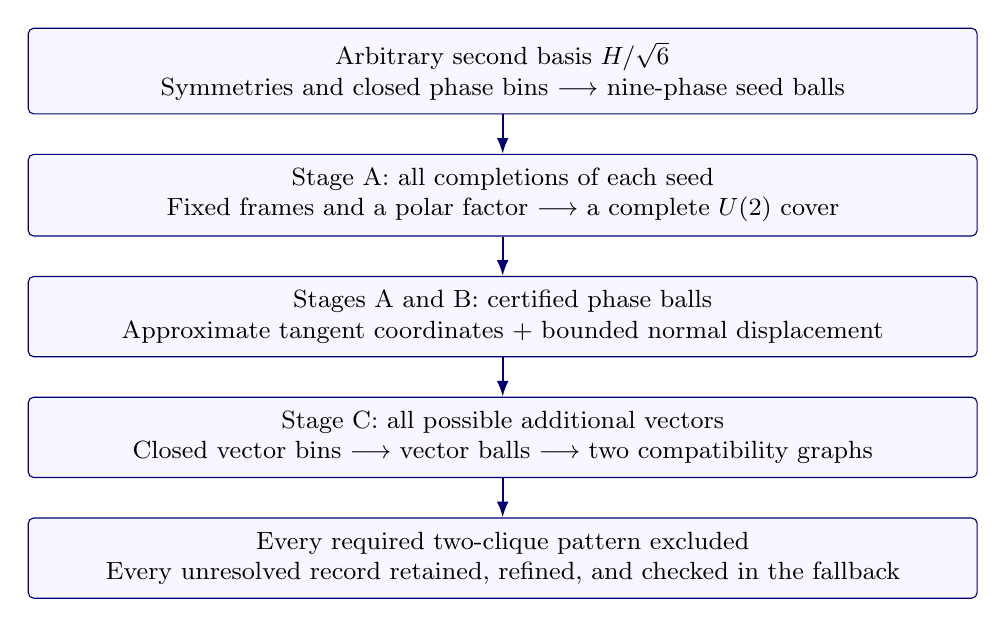
\begin{tikzpicture}[node distance=5mm,
 box/.style={draw=blue!45!black,rounded corners=2pt,fill=blue!3,
 text width=11.7cm,align=center,inner sep=5pt,font=\small},
 arr/.style={-{Latex[length=2mm]},thick,blue!45!black}]
\node[box] (seed) {Arbitrary second basis $H/\sqrt6$\\
Symmetries and closed phase bins $\longrightarrow$ nine-phase seed balls};
\node[box,below=of seed] (polar) {Stage A: all completions of each seed\\
Fixed frames and a polar factor $\longrightarrow$ a complete $U(2)$ cover};
\node[box,below=of polar] (phase) {Stages A and B: certified phase balls\\
Approximate tangent coordinates + bounded normal displacement};
\node[box,below=of phase] (graph) {Stage C: all possible additional vectors\\
Closed vector bins $\longrightarrow$ vector balls $\longrightarrow$ two compatibility graphs};
\node[box,below=of graph] (end) {Every required two-clique pattern excluded\\
Every unresolved record retained, refined, and checked in the fallback};
\draw[arr] (seed)--(polar);\draw[arr] (polar)--(phase);
\draw[arr] (phase)--(graph);\draw[arr] (graph)--(end);
\end{tikzpicture}
\caption{The proof preserves every exact candidate through successive
covers. An exclusion removes a region only after a necessary condition
fails with its certified margin. The execution documented in
Section~\ref{execute:observed} supplies the finite coverage and
terminal-exclusion premises of
Theorem~\ref{execute:finite-theorem}.}
\label{fig:proof-flow}
\end{figure}


The distinction between proposing a numerical object and certifying it
is used throughout. A floating-point center need not be an exact
Hadamard matrix. A computed small eigenspace need not parametrize a
component. A numerical linear solve need not be accurate: its output
is accepted only when a separate bound verifies the required
inequality. Every rejection uses a necessary condition with an
explicit safety margin. A failed certification or an exhausted search
cap retains an unresolved region; it cannot prove nonexistence.

All interval cells may be taken closed. Their overlap, repeated phase
representatives, and redundant balls or graph vertices can weaken the
exclusion but do not omit a possible configuration. The arithmetic
premises are stated, and the finite ranges and rounding margins are
proved, in \cref{sec:rounding}. The accompanying execution and build archives,
identified in \texttt{verification/computation/README.md}, preserve the evidence for
the fresh run documented in Section~\ref{execute:observed}. This proof
uses that run. The separate September 7 execution reported in the source
manuscript has not been authenticated here.

\subsection{The elementary lower bound}

The lower bound uses only the tensor-product construction mentioned
above. We give it explicitly to separate attainment of three bases from
the computer-assisted exclusion of four.

\begin{lemma}[Three mutually unbiased bases in dimension six]
\label{lem:three-mub-six}
There exist three pairwise mutually unbiased orthonormal bases in
$\mathbb C^6$.
\end{lemma}

\begin{proof}
Identify $\mathbb C^6$ with $\mathbb C^2\otimes\mathbb C^3$ in the standard
product coordinates. Define
\[
A_0=I_2,\qquad
A_1=\frac1{\sqrt2}\begin{pmatrix}1&1\\1&-1\end{pmatrix},\qquad
A_2=\frac1{\sqrt2}\begin{pmatrix}1&1\\i&-i\end{pmatrix}.
\]
These matrices are unitary, and for $r\ne s$ every entry of $A_r^*A_s$
has squared modulus $1/2$; the only cross product that is not immediate
from the entries is
\[
A_1^*A_2=\frac12\begin{pmatrix}1+i&1-i\\1-i&1+i\end{pmatrix}.
\]
Let $\omega=e^{2\pi i/3}$, and set
\[
F=\frac1{\sqrt3}(\omega^{jk})_{j,k=0}^{2},\qquad
D=\operatorname{diag}(1,\omega,\omega),\qquad
B_0=I_3,\quad B_1=F,\quad B_2=DF.
\]
The identity $1+\omega+\omega^2=0$ shows that $F$ is unitary; $D$ is
unitary as well. Both $F$ and $DF$ have entries of squared modulus $1/3$.
For their cross product,
\[
(F^*DF)_{jk}=\frac13\sum_{x=0}^{2}\omega^{x^2+(k-j)x}.
\]
If $t=k-j$ is read modulo $3$, the sum on the right is $1+2\omega$ for
$t=0$ and $2+\omega^2$ for $t=1,2$. Each has squared modulus $3$.
Consequently every entry of $B_r^*B_s$ has squared modulus $1/3$ when
$r\ne s$.

For $r=0,1,2$, let the columns of $U_r=A_r\otimes B_r$ form the $r$th
basis. Each $U_r$ is unitary. For $r\ne s$,
\[
U_r^*U_s=(A_r^*A_s)\otimes(B_r^*B_s),
\]
so every entry has squared modulus $(1/2)(1/3)=1/6$. Thus these three
bases are mutually unbiased, and $U_0=I_6$.
\end{proof}

\subsection{A Lie-algebra consequence}

An orthonormal basis $\mathcal B$ of $\C^6$ determines the Cartan
subalgebra $\mathfrak h_{\mathcal B}$ of traceless matrices diagonal
in that basis. It is spanned by the matrices $bb^*-I/6$ for
$b\in\mathcal B$. The Killing form on $\mathfrak{sl}_6(\C)$ is
$K(X,Y)=12\operatorname{tr}(XY)$; two subalgebras are
\emph{Killing-orthogonal} when this form vanishes between them. For
unit vectors $b,c$,
\[
 \operatorname{tr}\bigl((bb^*-I/6)(cc^*-I/6)\bigr)
 =|\langle b,c\rangle|^2-\frac16.
\]
Thus two bases are mutually unbiased exactly when their associated
Cartan subalgebras are Killing-orthogonal. These algebras are closed
under the standard adjoint, and the converse correspondence uses this
same adjoint condition.

\begin{corollary}[Adjoint-closed Cartan subalgebras]
\label{cor:adjoint-cartan}
Under the arithmetic and compiler conditions of
Appendix~\ref{sec:rounding}, using the complete execution documented in
Section~\ref{execute:observed} as in Theorem~\ref{thm:main},
the maximum number of pairwise Killing-orthogonal Cartan subalgebras of
$\mathfrak{sl}_6(\C)$ that are all closed under the same standard adjoint
$X\mapsto X^*=\overline X^{\,T}$ is three.
\end{corollary}

\begin{proof}
By \cite[Theorem~5.2]{BoykinSitharamTiepWocjan2005}, such collections of
Cartan subalgebras correspond to collections of mutually unbiased
orthonormal bases of the same cardinality. Theorem~\ref{thm:main} gives the
upper bound under its stated contract, and Lemma~\ref{lem:three-mub-six}
gives attainment.
\end{proof}

\section{Equivalences and an exhaustive seed cover}
\label{sec:seed}

The goal is to replace every possible second basis by one of finitely
many nine-phase seed balls. Closed phase discretization and necessary
compatibility tests follow the approach of
\cite[Section~3]{JamingEtAl2009} and
\cite[Sections~2--3]{JamingMatolcsiMora2010}. The symmetry reduction and
shared-coordinate estimates below prove completeness of this particular
seed cover.

We use phases in cycles and write
\[
 e(t)=\exp(2\pi i t),\qquad t\in\mathbb R,
\]
with entrywise application to vectors and matrices.  Matrix indices run from
$0$ to $5$, and a phase matrix is stored in row-major order, with $(i,j)$
in position $6i+j$.  The Hermitian inner product is
$\langle u,v\rangle=\sum_j\overline{u_j}v_j$, and $A^*$ denotes conjugate
transpose.  Vectors have their Euclidean norms; a matrix regarded as a phase
or displacement vector has Frobenius norm $\|\cdot\|_F$.  The notation
$\|\cdot\|_{\mathrm{op}}$ denotes the induced Euclidean operator norm.
We identify a complex equation with its real and imaginary parts, in that
order, so that a complex scalar and its realification have the same norm.
An angle is in radians only when this is stated explicitly.

\subsection{Equivalences and phase gauges}

\begin{definition}
\label{seed:extendibility}
A matrix $H\in\mathbb C^{6\times6}$ is a complex Hadamard matrix here if
every entry has modulus one and $HH^*=6I$.  It is \emph{extendible} if the
standard basis and the columns of $H/\sqrt6$ belong to a family of four
mutually unbiased orthonormal bases.
\end{definition}

A common unitary maps the first member of any proposed family to the
standard basis.  Unbiasedness to that basis forces the entries of the second
basis matrix to have modulus $1/\sqrt6$.  Thus it is $H/\sqrt6$ for a matrix
as in Definition~\ref{seed:extendibility}; since $H$ is square, $HH^*=6I$
also gives $H^*H=6I$.  Every such $H$ admits a real phase lift $P$ with
$H=e(P)$.

\begin{lemma}[Equivalences]
\label{seed:equivalences}
Extendibility is invariant under row or column permutations, multiplication
of rows or columns by unit scalars, complex conjugation, and transposition.
\end{lemma}

\begin{proof}
Permuting or rephasing columns only changes the order or phases of vectors
within the second basis.  A row permutation or row rephasing is a common
unitary operation on all four bases; it preserves the standard basis up
to the same irrelevant changes.  Complex conjugation preserves both
orthogonality and the moduli of inner products.

For transposition, put $U=H/\sqrt6$.  Apply the common unitary $U^*$ to a
family whose first two basis matrices are $I,U$.  These two matrices become
$U^*,I$.  Interchange their roles and conjugate every coordinate.  The first
two matrices are now $I,U^T$.  All these operations are reversible, which
proves the assertion in both directions.
\end{proof}

The transposition argument applies to an exact Hadamard matrix.  It does
not assert that an approximate center supplies a unitary change of basis.

For a real $6$-by-$6$ matrix $z$, define double centering by
\begin{equation}
\label{seed:projection-formula}
 (\Pi z)_{ij}
 =z_{ij}-\frac16\sum_bz_{ib}-\frac16\sum_az_{aj}
       +\frac1{36}\sum_{a,b}z_{ab}.
\end{equation}
Its range is the \emph{horizontal} subspace of matrices with every row sum
and every column sum zero.  We also use unwrapped dephasing,
\begin{equation}
\label{seed:dephasing-formula}
 D_0(P)_{ij}=P_{ij}-P_{i0}-P_{0j}+P_{00}.
\end{equation}

\begin{lemma}[Horizontal phase representatives]
\label{seed:horizontal}
The map $\Pi$ is the orthogonal projection onto the horizontal subspace.
In particular, $\|\Pi z\|_F\le\|z\|_F$.  If two phase representatives have
difference $z$, the second is equivalent under row and column rephasings
to the first plus $\Pi z$.  This statement remains valid after arbitrary
entrywise integer changes of phase representatives.
\end{lemma}

\begin{proof}
Formula~\eqref{seed:projection-formula} has zero row and column sums, and
$z-\Pi z$ is a sum of a matrix constant on each row and a matrix constant
on each column.  Every such sum is orthogonal to the horizontal subspace
in the real Frobenius inner product.  This proves the projection assertion
and its norm bound.  If $Q=P+z$, then
$P+\Pi z=Q-(z-\Pi z)$ differs from $Q$ by row and column phases, which are
allowed by Lemma~\ref{seed:equivalences}.  Entrywise integer additions
leave $e(P)$ unchanged.
\end{proof}

Likewise, $D_0(P)$ gives an equivalent matrix with first row and column
phases zero.  When a wrapped difference is used, its chosen integers define
legitimate phase representatives.  No argument requires a rounded decision
at a half-integer to agree with a uniquely preferred nearest representative.

\subsection{A symmetry arrangement for nine phases}

The \emph{gap} of a finite circular multiset is its largest circular gap.
Equivalently, it is the greatest length of an open arc containing no point
of the multiset.  Points are counted with multiplicity when sorted; a
repeated point contributes a zero gap.  For each pair of distinct rows
of $P$, consider their six phase differences modulo one, and do the same
for each pair of distinct columns.

\begin{lemma}[Seed arrangement]
\label{seed:arrangement}
Every exact Hadamard matrix has an equivalent dephased representative for
which a pair of rows attaining the minimum gap among all row and column
pairs is the first pair, and its phases can be written
\begin{equation}
\label{seed:x-arrangement}
 x=(0,x_1,x_2,x_3,x_4,x_5),\qquad
 0\le x_1\le\cdots\le x_5\le1,\qquad
 g_x=1-x_5,\qquad x_1\le x_5-x_4.
\end{equation}
After any one of these five noninitial columns is selected and moved to
second position, the last four rows can be permuted so that the second
column has phases
\begin{equation}
\label{seed:y-arrangement}
 y=(0,\xi,y_2,y_3,y_4,y_5),\qquad
 0\le y_2\le y_3\le y_4\le y_5\le1,
\end{equation}
where $\xi$ is the selected entry of $x$.  These lists satisfy
\begin{equation}
\label{seed:local-conditions}
 \sum_{j=0}^5 e(x_j)=0,\qquad
 \sum_{j=0}^5 e(y_j)=0,\qquad g_y\ge g_x.
\end{equation}
\end{lemma}

\begin{proof}
There are finitely many row and column pairs, so a pair of minimum gap
exists.  Transpose if it is a column pair, and permute rows to make it the
first pair.  Choose one of its largest gaps, start the circular ordering
immediately after that gap, and use this starting point as the first
column.  Dephase the first row and column.  Ordering the remaining columns
along the complementary arc gives $g_x=1-x_5$ and the sorted list in
\eqref{seed:x-arrangement}.

If the final orientation inequality fails, interchange the two selected
rows, use the old $x_5$ column as the starting column, and reverse the
ordering.  The new list is
\[
 x'_0=0,\qquad x'_i=x_5-x_{5-i}\quad(1\le i\le5).
\]
It has the same distinguished largest gap, and
$x'_1=x_5-x_4$ whereas $x'_5-x'_4=x_1$.  Thus this orientation satisfies
the required inequality whenever the former one does not.  The construction
uses a chosen largest gap and is unchanged in validity by ties or repeated
points.

Select a noninitial column and place it second.  Permuting the last four
rows sorts its last four phase entries, without changing either of the first
two rows.  Orthogonality of those rows gives the first vanishing sum in
\eqref{seed:local-conditions}; orthogonality of the first two columns gives
the second.  Row and column rephasings rotate the relevant difference
multisets; permutations merely reorder points or relabel pairs.  Transposition
interchanges the two collections of pairs.  Consequently their minimum
gap remains $g_x$, and the newly selected column pair has $g_y\ge g_x$.
\end{proof}

Set $N=112$ and $w=1/N$.  All bins are closed:
\begin{equation}
\label{seed:bins}
 I_b=[b/N,(b+1)/N],\qquad
 u_b=(b+1/2)/N,\qquad 0\le b<N.
\end{equation}
They cover $[0,1]$, including both endpoints.  Assignments at shared
boundaries need not be unique.  Sorted exact phases admit nondecreasing
bin indices, so write the five indices for $x_1,\ldots,x_5$ as
\[
 b^X=(a,b,c,d,l),\qquad 0\le a\le b\le c\le d\le l<N.
\]
The orientation condition implies the necessary integral restriction
\begin{equation}
\label{seed:orientation-filter}
 \frac aN\le x_1\le x_5-x_4\le\frac{l+1-d}{N},
 \qquad a\le l-d+1.
\end{equation}

For this index tuple choose $s\in\{0,\ldots,4\}$ as the first minimizer of
$|2b^X_s+1-N|$.  This is the rule in \texttt{seeds::mk}.  Its selected
original column is $s+1$, its selected exact phase is $\xi=x_{s+1}$, and
the new column order is the original column zero, column $s+1$, and the
other four columns in their former order.  This selection only specifies
a column; it imposes no further condition on $\xi$.

After arranging $y$ as in \eqref{seed:y-arrangement}, its five varying
entries have bins
\[
 b^Y=(b^X_s,b^Y_1,b^Y_2,b^Y_3,b^Y_4),\qquad
 0\le b^Y_1\le b^Y_2\le b^Y_3\le b^Y_4<N.
\]
The shared entry uses precisely the same bin as in $x$; it is not required
to be ordered relative to the four tail bins.

\begin{lemma}[Stability of circular gaps]
\label{seed:gap-stability}
If each point of one circular multiset is matched to a point of another
at circular distance at most $\delta$, their gaps differ by at most
$2\delta$.
\end{lemma}

\begin{proof}
Take an empty open arc of length $L$ in the first multiset.  If $L>2\delta$,
trim $\delta$ from each end.  A point of the second multiset inside the
remaining open arc would have its matched first point in the original
empty arc, a contradiction.  Hence the second gap is at least
$L-2\delta$.  If $L\le2\delta$, the same lower bound follows from
nonnegativity.  Apply this to a largest gap and then interchange the
two multisets.  No preservation of the sorted order is used.
\end{proof}

\begin{lemma}[Necessary midpoint gap filters]
\label{seed:gap-filters}
For every bin pair containing lists as in Lemma~\ref{seed:arrangement},
the midpoint gaps, including the fixed zero, satisfy
\begin{equation}
\label{seed:gap-inequalities}
 g_{x,\mathrm{mid}}\le1-\frac{l-1}{N},\qquad
 g_{y,\mathrm{mid}}\ge1-\frac{l+2}{N}.
\end{equation}
\end{lemma}

\begin{proof}
Each varying phase is within $w/2$ of its midpoint, and the initial zero
is unchanged.  Lemma~\ref{seed:gap-stability} bounds each gap change by $w$.
Since $x_5\in[l/N,(l+1)/N]$, we have
$1-(l+1)/N\le g_x\le1-l/N$.  Combining these inequalities with
$g_y\ge g_x$ proves both assertions.
\end{proof}

For sorted midpoint bin indices $q_0,\ldots,q_4$, the gap used by
\texttt{mk} is
\[
 \max\left\{\frac{q_0+1/2}{N},
 \frac{q_1-q_0}{N},\ldots,\frac{q_4-q_3}{N},
 1-\frac{q_4+1/2}{N}\right\}.
\]
For a $Y$ tuple it sorts a copy solely for this computation, preserving
the stored shared-first ordering.

\subsection{Vanishing-sum filters and the shared displacement}

For either list, let $u=(u_0,\ldots,u_4)$ be its five varying midpoints.
Define the real two-vector $c$ and real $2$-by-$5$ matrix $J$ by
\begin{equation}
\label{seed:residual-data}
 c=\frac{1+\sum_{j=0}^4e(u_j)}{2\pi i},\qquad J_j=e(u_j),
\end{equation}
using realification in both definitions.

\begin{lemma}[Necessary sum test]
\label{seed:sum-test}
If $1+\sum_{j=0}^4e(u_j+\Delta_j)=0$ and $|\Delta_j|\le w/2$, then
\begin{equation}
\label{seed:taylor-residual}
 \|c+J\Delta\|\le\frac{5\pi w^2}{4}.
\end{equation}
In particular, for every $v\in\mathbb R^2$,
\begin{equation}
\label{seed:sum-support}
 |v\cdot c|\le\frac{5\pi w^2}{4}\|v\|
                  +\frac w2\sum_{j=0}^4|v\cdot J_j|.
\end{equation}
\end{lemma}

\begin{proof}
The second derivative of $e(t)$ has modulus $4\pi^2$.  Taylor's formula
with integral remainder therefore gives
\[
 \left|\frac{e(u_j+\Delta_j)-e(u_j)}{2\pi i}
             -e(u_j)\Delta_j\right|\le\pi\Delta_j^2.
\]
Sum the five remainders and use the vanishing-sum hypothesis to obtain
\eqref{seed:taylor-residual}.  Taking the dot product with $v$, followed
by the triangle inequality and $|\Delta_j|\le w/2$, gives
\eqref{seed:sum-support}.
\end{proof}

The function \texttt{sumok} tests \eqref{seed:sum-support} in the residual
direction and in directions perpendicular to the five unit-exponential
columns.  The inequality holds for every real direction, so their numerical
construction need not reproduce any prescribed exact direction.  The
one-sided margins for evaluating the residuals and supports are established
in Section~\ref{sec:rounding}.

In grid units $h=N\Delta$, write
\begin{equation}
\label{seed:grid-error}
 E=\frac{5\pi}{4N},\qquad \|Jh+Nc\|\le E,
 \qquad |h_j|\le\frac12.
\end{equation}

\begin{lemma}[Shared-coordinate intervals]
\label{seed:shared-interval}
Let $t$ be the position of a shared entry in one of the two lists.  Every
feasible displacement satisfies, for each $v\in\mathbb R^2$,
\begin{equation}
\label{seed:clip-inequality}
 |Nv\cdot c+(v\cdot J_t)h_t|
 \le E\|v\|+\frac12\sum_{j\ne t}|v\cdot J_j|.
\end{equation}
If $a=v\cdot J_t\ne0$ and the right side is $r$, this is the closed
interval constraint
\begin{equation}
\label{seed:clip-interval}
 -\frac{Nv\cdot c}{a}-\frac r{|a|}
 \le h_t\le
 -\frac{Nv\cdot c}{a}+\frac r{|a|}.
\end{equation}
The intervals obtained for the shared entry from $X$ and $Y$ must intersect.
\end{lemma}

\begin{proof}
Separate the shared term in \eqref{seed:grid-error}, take its dot product
with $v$, and bound each remaining coordinate by $1/2$.  Solving the
resulting absolute-value inequality gives \eqref{seed:clip-interval} for
either sign of $a$.  The shared midpoint is identical in both lists, so
the same exact grid displacement belongs to both sets of necessary
intervals.
\end{proof}

The function \texttt{extend} begins with $[-1/2,1/2]$ and intersects these
constraints, using the shared column direction and directions perpendicular
to the other four columns.  Here $t=s$ for $X$ and $t=0$ for $Y$.
It omits divisors of magnitude below $10^{-6}$, which only removes a
constraint.  Numerator and endpoint margins enlarge the computed intervals,
as proved in Section~\ref{sec:rounding}.  The pair is rejected only when
the two resulting intervals are strictly disjoint; a common endpoint is
retained.

The enumeration in \texttt{seeds::build} now has an explicit interpretation.
It visits every weakly increasing five-bin $X$ tuple and applies
\eqref{seed:orientation-filter}, the first inequality in
\eqref{seed:gap-inequalities}, and \texttt{sumok}.  Separately, for every
possible first bin it visits all weakly increasing four-bin $Y$ tails and
applies \texttt{sumok}.  The program \texttt{covout} matches the shared
bin, applies the second gap inequality, and intersects the shared
displacement intervals.  Every discarded exact solution would therefore
violate one of the necessary conditions just proved.  The numerical gap
comparisons include outward slack, treated in Section~\ref{sec:rounding}.

\subsection{Certified reuse of seed centers}

The nine seed coordinates, before moving the selected column, are
\begin{equation}
\label{seed:nine-coordinates}
 q=(x_1,x_2,x_3,x_4,x_5,y_2,y_3,y_4,y_5)\in\mathbb R^9.
\end{equation}
For a bin pair let $u\in\mathbb R^9$ be its rational midpoint and put
$h=N(q-u)$.  Thus $h\in[-1/2,1/2]^9$; the shared displacement is $h_s$.
Retaining $u$ as a center would cover the entire bin with radius
$3/(2N)<0.032$.  To reduce the number of centers, we instead test whether
its feasible portion lies in a radius-$0.032$ ball about a previously
retained midpoint.  If no such test succeeds, we retain $u$.

Let $J_X,J_Y,c_X,c_Y$ denote the data in
\eqref{seed:residual-data}.  Define a real $4$-by-$9$ matrix $J_*$ by
specifying its action:
\begin{equation}
\label{seed:stacked-system}
 J_*h=\begin{pmatrix}
 J_X(h_0,h_1,h_2,h_3,h_4)^T\\
 J_Y(h_s,h_5,h_6,h_7,h_8)^T
 \end{pmatrix},\qquad
 p_*=\begin{pmatrix}-Nc_X\\-Nc_Y\end{pmatrix}.
\end{equation}
For feasible $h$ we have $J_*h=p_*+r_*$, where the two real two-vector
blocks $r_X,r_Y$ of $r_*$ satisfy $\|r_X\|,\|r_Y\|\le E$.

\begin{lemma}[Support bounds for center reuse]
\label{seed:dual-support}
Let $u'$ be a previously retained midpoint with the same selected position
$s$, and let $k=N(u-u')\in\mathbb Z^9$.  Every feasible displacement in
the current bin pair satisfies
\begin{equation}
\label{seed:distance-bound}
 N^2\|q-u'\|^2=\|k+h\|^2
 \le\|k\|^2+\frac94+2k\cdot h.
\end{equation}
Two upper bounds for the last term are
\begin{align}
 2k\cdot h&\le\sum_{j=0}^8|k_j|,
 \label{seed:box-support}\\
 2k\cdot h&\le
 \sum_{j=0}^8|k_j-(J_*^Tv)_j|
 +2v\cdot p_*+2E(\|v_X\|+\|v_Y\|),
 \qquad v\in\mathbb R^4,
 \label{seed:dual-formula}
\end{align}
where $v_X,v_Y$ are the two real two-vector blocks of $v$.
\end{lemma}

\begin{proof}
Expand the square in \eqref{seed:distance-bound} and use
$\|h\|^2\le9/4$.  The coordinate bounds give
\eqref{seed:box-support}.  For the other bound, write
\[
 2k\cdot h
 =2(k-J_*^Tv)\cdot h+2v\cdot p_*+2v\cdot r_*.
\]
The first term is at most $\sum_j|k_j-(J_*^Tv)_j|$ by the same coordinate
bounds.  Cauchy--Schwarz on the two residual blocks bounds the last term
by $2E(\|v_X\|+\|v_Y\|)$.
\end{proof}

The function \texttt{supdual} proposes vectors $v$ and evaluates the right
side of \eqref{seed:dual-formula}.  The validity of a proposal does not
depend on how it was generated or on the accuracy of the heuristic linear
solve.  Only finite proposed components of magnitude at most $10^4$ are
used.  Its evaluation replaces $1.25\pi/N$ by the larger $1.251\pi/N$
and adds a final support margin.  Section~\ref{sec:rounding} proves that
the resulting bound is conservative.

Set $R=0.032$.  For a proposed previous center, \texttt{testBucket} first
tries \eqref{seed:box-support}, and then, if applicable, the dual bound.
It returns success only when the resulting upper bound in
\eqref{seed:distance-bound} is below the safely lowered comparison
threshold for $(NR)^2$.  Hence success certifies the entire feasible
portion of the current bin pair, rather than just its midpoint.
Distance cutoffs, bucket indices, and reach tests only decide which previous
centers to try.  Omitting a possible previous center cannot produce a
successful coverage test.

For clarity, the shared column is counted once in
\eqref{seed:nine-coordinates}, although its displacement enters both
equations in \eqref{seed:stacked-system}.  Reuse requires equality of the
selected \emph{position} $s$.  Moving that position to the start of the
five $X$ coordinates then applies the same coordinate permutation to the
current point and the retained center, and preserves their Euclidean
distance.  The resulting order is the selected $X$ entry, the other four
$X$ entries in order, and the four $Y$ tail entries.  These are precisely
the nine entries of the dephased first two rows and columns used in the
next stage.  Centers retained earlier for the same $X$ tuple are handled
identically, with the first five components of $k$ zero.

\begin{proposition}[Exhaustive seed cover]
\label{seed:cover}
For a completed execution of the specified \texttt{covout} traversal
under the arithmetic conditions of Section~\ref{sec:rounding}, the written
rational midpoint centers, each with its recorded selected position, cover
the seed coordinates of every exact complex Hadamard matrix up to the
equivalences of Lemma~\ref{seed:equivalences}, by closed Euclidean balls
of radius $0.032$.  After the indicated column ordering and conversion of
the centers to binary phase values, radius $0.0320001$ is sufficient.
\end{proposition}

\begin{proof}
Given an exact Hadamard matrix, first use
Lemma~\ref{seed:arrangement} to arrange $x$.  Choose a nondecreasing closed
bin assignment, determine $s$ from that tuple, and then arrange and assign
$y$ with the same shared bin.  All these choices exist also on bin
boundaries and at repeated phases.  The tuple is present in the stated
enumeration.  Lemmas~\ref{seed:gap-filters}, \ref{seed:sum-test}, and
\ref{seed:shared-interval}, together with their certified outward numerical
margins, ensure that its bin pair is not rejected by a necessary filter.

Consider the retained centers as the remaining bin pairs are traversed.
If a coverage test succeeds, Lemma~\ref{seed:dual-support} and the certified
comparison margins put every feasible point of the current pair in a
radius-$R$ ball about an already retained center.  If no test succeeds,
the program retains the current midpoint itself.  Its distance from any
point of its full nine-dimensional bin is at most
\[
 \frac{\sqrt9}{2N}=\frac{3}{224}<0.032.
\]
Thus, by induction over the traversal, the retained centers cover every
feasible point in every processed pair.  Restricting the attempted reuse
centers can only cause further midpoint insertions.  Previously retained
centers remain retained and are included in the output.

The common selected-position permutation preserves all these distances.
Finally, Section~\ref{sec:rounding} bounds the joint error of the nine
binary midpoint phases by less than $10^{-14}$.  The triangle inequality
therefore permits the enlarged radius $0.0320001$.  The centers need not
themselves satisfy the exact Hadamard equations; their balls cover the
necessary seed coordinates of all exact solutions.
\end{proof}

\section{Completion over a fixed seed ball}
\label{sec:completion}

This section supplies necessary conditions for a dephased Hadamard matrix
whose nine seed phases lie in one prescribed ball.  It reduces the remaining
completion problem to a covering of $U(2)$.  The reduction uses frames fixed
at the seed center; no exact Hadamard matrix is assumed to occur at that
center.  All statements in this section first concern exact real and
complex arithmetic.  The implementation uses the outward replacements and
comparison margins justified in Section~\ref{sec:rounding}.

\subsection{Seed blocks and fixed complementary frames}

Fix the stored seed center, taking its binary phase coordinates as exact
real numbers.  After moving the shared column into the second position,
write its relevant unit entries as $a,b_0,\ldots,b_3,c_0,\ldots,c_3$, and put
\begin{equation}
\label{completion:seed-blocks}
 E_0=\begin{pmatrix}1&1\\1&a\end{pmatrix},\qquad
 B_0=\begin{pmatrix}1&1&1&1\\b_0&b_1&b_2&b_3\end{pmatrix},\qquad
 (C_0)_{i,:}=(1,c_i).
\end{equation}
A feasible completion is an entrywise unit-modulus matrix
\[
 H'=\begin{pmatrix}E'&B'\\ C'&D'\end{pmatrix},\qquad
 H'H'^*=H'^*H'=6I,
\]
with first row and first column equal to one.  Its seed displacements,
measured in radians, are ordered as
\[
 s=(s_a,s_{b_0},\ldots,s_{b_3},s_{c_0},\ldots,s_{c_3})\in\R^9.
\]
Thus the varied entries are $a e^{i s_a}$, $b_j e^{i s_{b_j}}$, and
$c_i e^{i s_{c_i}}$.  The shared entry occurs once in $s$.  With zero-based
row-major phase indexing, these coordinates occupy
\begin{equation}
\label{completion:position-map}
 (7,8,9,10,11,13,19,25,31).
\end{equation}
The enlarged seed radius in cycles is denoted by $r_s$, and
$R_s=2\pi r_s$.  In the stated computation $r_s=.0320001$.
Set $\Delta E=E'-E_0$, and define $\Delta B,\Delta C$ similarly.  To avoid
confusing norms with entries of the blocks, write
\[
 e_1=\lVert\Delta E\rVert_F,\qquad
 b_1'=\lVert\Delta B\rVert_F,\qquad
 c_1'=\lVert\Delta C\rVert_F.
\]
The chord bound $|e^{ix}-1|\le |x|$ gives
\begin{equation}
\label{completion:seed-norm}
 e_1^2+(b_1')^2+(c_1')^2\le\lVert s\rVert^2\le R_s^2.
\end{equation}

\begin{lemma}[Fixed frames]
\label{completion:frames}
Let $p\in\C^4$ have unit-modulus entries, let
$S=\sum_j p_j$, and set $M=(\mathbf 1\ p)$.  The squared singular values
of $M$ are $4\pm |S|$.  If $|S|<4$, then
\begin{equation}
\label{completion:inverse-frame}
 M(M^*M)^{-1}
 =\frac1{16-|S|^2}
 \big(4\mathbf 1-p\overline S\,,\;4p-\mathbf 1 S\big).
\end{equation}
Under the same condition $|S|<4$, there is an orthonormal $4$-by-$2$
matrix $K$ with range $\ker M^*$.
It may be constructed by completing $\mathbf 1/2$ and the normalized
residual of $p$ by projected coordinate vectors with nonzero residuals.
\end{lemma}

\begin{proof}
Direct multiplication gives
\[
 M^*M=\begin{pmatrix}4&S\\\overline S&4\end{pmatrix}.
\]
Its eigenvalues and inverse give the assertions about singular values and
\eqref{completion:inverse-frame}.  The first two Gram--Schmidt vectors
span $\operatorname{ran}M$.  At each subsequent step, the orthogonal
complement of the vectors already selected is nonzero.  Since the coordinate
vectors span $\C^4$, at least one has a nonzero projection into that
complement.  Selecting and normalizing such a projection gives the next
orthonormal vector.  The final two vectors form $K$.
\end{proof}

Apply Lemma~\ref{completion:frames} to $p=(\overline b_j)_j$ and
$p=(c_i)_i$.  Throughout the seed ball keep the resulting frames fixed, and
write
\begin{equation}
\label{completion:frame-definitions}
 G_B=B_0^*(B_0B_0^*)^{-1},\qquad
 G_C=C_0(C_0^*C_0)^{-1},\qquad
 \operatorname{ran}K_B=\ker B_0,\quad
 \operatorname{ran}K_C=\ker C_0^*.
\end{equation}
Here $K_B^*K_B=K_C^*K_C=I_2$.  Define
\[
 m_B=\sigma_{\min}(B_0),\quad
 m_C=\sigma_{\min}(C_0),\quad
 m=\min(m_B,m_C)>0,
\]
so that $\lVert G_B\rVert_{\rm op}=1/m_B$ and
$\lVert G_C\rVert_{\rm op}=1/m_C$.
The numerical construction chooses particular coordinate vectors; the ideal
frames in this argument use those same choices.  The acceptance checks on
rank and residual norms certify that this construction is defined.  A
failed frame check leaves the seed unresolved and never excludes it.

We shall use the orthogonal projections
\begin{equation}
\label{completion:projections}
 P_K=K_BK_B^*,\qquad P_B=I-P_K=G_BB_0,\qquad
 P_C=I-K_CK_C^*=G_CC_0^*.
\end{equation}
Finally, put
\begin{equation}
\label{completion:A-bounds}
 A_0=\lVert E_0\rVert_{\rm op}=\sqrt{2+|1+a|},\qquad
 A_* =\min(2,A_0+R_s).
\end{equation}
Both $A_0$ and $\lVert E'\rVert_{\rm op}$ are at most $A_*$.
Indeed $A_0\le2$, every entry of $E'$ has modulus one and hence
$\lVert E'\rVert_{\rm op}\le\lVert E'\rVert_F=2$, and
$\lVert E'\rVert_{\rm op}\le A_0+e_1\le A_0+R_s$.

\subsection{A unitary associated to every feasible completion}

The polar decomposition associates a unitary with a nonsingular square
matrix, and its nearest-unitary property in unitarily invariant norms is
classical~\cite[Theorem~1]{FanHoffman1955}; see also
\cite[Theorem~1.1 and Corollary~2.3]{Higham1986Polar}. Here the compressed
completion has an explicit positive defect. The next lemma derives the
trace-defect estimate required for the finite $U(2)$ cover.


\begin{lemma}[Polar comparison]
\label{completion:polar}
For a feasible completion let $Y=K_C^*D'K_B$.  Then
\begin{align}
\label{completion:deficit-identity}
 6I-Y^*Y
 &=K_B^*B'^*B'K_B+
   K_B^*D'^*P_CD'K_B\succeq0,\\
\label{completion:deficit-bound}
 \operatorname{tr}(6I-Y^*Y)
 &\le (b_1')^2+
 \frac{(\lVert E'\rVert_{\rm op}b_1'+\sqrt6\,c_1')^2}{m_C^2}
 \le q,
\end{align}
where
\begin{equation}
\label{completion:q-and-p}
 q=R_s^2\left(1+\frac{A_*^2+6}{m_C^2}\right).
\end{equation}
If $q<6$, the polar factor
$V=Y(Y^*Y)^{-1/2}$ belongs to $U(2)$ and satisfies
\begin{equation}
\label{completion:polar-bound}
 \lVert Y-\sqrt6 V\rVert_F\le
 p:=\frac{q}{\sqrt6+\sqrt{6-q}}.
\end{equation}
\end{lemma}

\begin{proof}
The lower-right block of $H'^*H'=6I$ is
$B'^*B'+D'^*D'=6I$.  Compress it by $K_B$, and subtract
$Y^*Y=K_B^*D'^*(I-P_C)D'K_B$.  This proves
\eqref{completion:deficit-identity}.  Its trace is
\[
 \lVert B'K_B\rVert_F^2+\lVert P_CD'K_B\rVert_F^2.
\]
Since $B_0K_B=0$, the first term is at most $(b_1')^2$.
The off-diagonal block of column orthogonality gives
$C'^*D'=-E'^*B'$, and consequently
\[
 C_0^*D'K_B=-E'^*\Delta B K_B-\Delta C^*D'K_B.
\]
Now $P_C=G_CC_0^*$ and $\lVert D'\rVert_{\rm op}\le\sqrt6$.
These facts give the first inequality in \eqref{completion:deficit-bound}.
For the second, apply Cauchy--Schwarz to
$A_*b_1'+\sqrt6 c_1'$ and then use
\eqref{completion:seed-norm}.

Let $\ell_1,\ell_2$ be the eigenvalues of $6I-Y^*Y$.
They are nonnegative and have sum at most $q<6$.  The singular values of
$Y$ are therefore positive and equal to $\sqrt{6-\ell_j}$, so its polar
factor is unitary.  Moreover
\[
 \sqrt6-\sqrt{6-\ell_j}
 =\frac{\ell_j}{\sqrt6+\sqrt{6-\ell_j}}
 \le\frac{\ell_j}{\sqrt6+\sqrt{6-q}}.
\]
Taking the Euclidean norm of these two singular-value differences, and
using $\sqrt{\ell_1^2+\ell_2^2}\le\ell_1+\ell_2\le q$, proves
\eqref{completion:polar-bound}.
\end{proof}

The inequality $q<6$ is checked using outward bounds.  In the specified
parameter range the stronger bound $q<.32$ follows from the accepted frame
checks and the seed radius; see Section~\ref{sec:rounding}.  The reduction
therefore assigns at least one $V\in U(2)$ to every feasible completion of
an accepted seed ball.

\subsection{The unitary cells and their Taylor bounds}

\begin{lemma}[A closed covering of $U(2)$]
\label{completion:unitary-cover}
Every $V\in U(2)$ has a representation
\begin{equation}
\label{completion:unitary-parameterization}
 V=e(\alpha)
 \begin{pmatrix}
 e(\beta)\cos(2\pi t)&e(\gamma)\sin(2\pi t)\\
 -e(-\gamma)\sin(2\pi t)&e(-\beta)\cos(2\pi t)
 \end{pmatrix},
\end{equation}
with
$0\le\alpha\le\tfrac12$, $0\le t\le\tfrac14$, and
$0\le\beta,\gamma\le1$.
For an integer $N_u$ divisible by four, the products of closed intervals
of width $1/N_u$ in these ranges cover this parameter domain.  Their four
bin counts are $N_u/2,N_u/4,N_u,N_u$.
\end{lemma}

\begin{proof}
Choose a square root of $\det V$ having phase $\alpha\in[0,1/2]$ in
cycles.  Then $e(-\alpha)V\in SU(2)$ and has the form
\[
 \begin{pmatrix}z&w\\-\overline w&\overline z\end{pmatrix},
 \qquad |z|^2+|w|^2=1.
\]
Choose $t\in[0,1/4]$ with
$|z|=\cos(2\pi t)$ and $|w|=\sin(2\pi t)$, and choose phases $\beta$
and $\gamma$ for $z$ and $w$.  A phase of a zero entry may be chosen
arbitrarily.  Thus no boundary case requires division by an entry.
The interval products cover the stated closed domain directly.
\end{proof}

Fix one cell and denote its midpoint matrix by $U$.  If $V$ is represented
inside the cell, let
\begin{equation}
\label{completion:unitary-cell}
 \theta=(\theta_\alpha,\theta_t,\theta_\beta,\theta_\gamma),\qquad
 |\theta_j|\le h:=\frac{\pi}{N_u},
\end{equation}
be its displacement from the midpoint in radians.  Denote the midpoint
angular differential, applied to this displacement, by $dU[\theta]$.
All four derivatives here are with respect to radian angles, although
\eqref{completion:unitary-parameterization} uses cycle coordinates.

\begin{lemma}[Uniform cell Taylor estimates]
\label{completion:unitary-taylor}
For the cell and displacement in \eqref{completion:unitary-cell},
\begin{equation}
\label{completion:unitary-taylor-bounds}
 \lVert V-U\rVert_F\le\sqrt6 h,\qquad
 \lVert V-U-dU[\theta]\rVert_F\le\frac{\sqrt{42}}2h^2.
\end{equation}
\end{lemma}

\begin{proof}
Follow the straight segment in the four angle coordinates and write its
matrix as $U(\tau)$, $0\le\tau\le1$.  For this proof abbreviate the four
constant angular velocities as
$x=\theta_\alpha$, $y=\theta_t$, $z=\theta_\beta$, and
$w=\theta_\gamma$, and let $T$ be the current radian $t$ angle.
Differentiating the four entries yields
\[
 \lVert U'(\tau)\rVert_F^2
 =2\big(x^2+y^2+z^2\cos^2 T+w^2\sin^2 T\big)\le6h^2.
\]
For the two diagonal entries, the squared magnitudes of the real factors
in the second derivative have sum
\begin{align*}
 &\big(((x+z)^2+y^2)^2+((x-z)^2+y^2)^2\big)\cos^2 T\\
 &\qquad=2\big((x^2+z^2+y^2)^2+4x^2z^2\big)\cos^2 T
 \le26h^4\cos^2 T.
\end{align*}
The imaginary factors of those two entries contribute
\[
 4y^2\big((x+z)^2+(x-z)^2\big)\sin^2 T
 \le16h^4\sin^2 T.
\]
The off-diagonal entries give the same two bounds with $z$ replaced by $w$
and cosine and sine interchanged.  Real and imaginary factors add in
squared magnitude.  Hence $\lVert U''(\tau)\rVert_F^2\le42h^4$.
Integrating the first derivative, and then using the integral Taylor
remainder with weight $1-\tau$, proves
\eqref{completion:unitary-taylor-bounds}.
\end{proof}

For clarity about the implementation, if the entries of $U$ are $U_{ij}$,
its alpha derivative is $iU$, its beta derivative has diagonal entries
$iU_{00},-iU_{11}$ and zero off-diagonal entries, and its gamma derivative
has off-diagonal entries $iU_{01},-iU_{10}$ and zero diagonal entries.
The $t$ derivative differentiates the displayed sine and cosine factors.
These are precisely the four angular derivatives assembled by
\texttt{uc::init} and \texttt{uc::initDeriv}.

\subsection{Comparison with a cell center}

For the fixed seed and unitary cell define
\begin{equation}
\label{completion:comparison-def}
 D=D_{\rm span}+D_{\rm ker},\qquad
 D_{\rm span}=-C_0E_0^*G_B^*,\qquad
 D_{\rm ker}=\sqrt6 K_C U K_B^*,\qquad Z=D'-D.
\end{equation}
The symbol $D$ henceforth denotes this comparison block, which need not be
entrywise flat.  It is not asserted to be the lower block of a Hadamard
matrix at the seed center.

\begin{lemma}[Orthogonal comparison pieces]
\label{completion:comparison-pieces}
The matrices $ZP_B$, $P_CZP_K$, and $(I-P_C)ZP_K$ are pairwise
Frobenius-orthogonal and sum to $Z$.  They satisfy
\begin{align}
\label{completion:piece-B}
 ZP_B&=(-\Delta C E_0^*-C'\Delta E^*-D'\Delta B^*)G_B^*,\\
\label{completion:piece-C}
 P_CZP_K&=G_C(-E'^*\Delta B-\Delta C^*D')P_K,\\
\label{completion:piece-K}
 (I-P_C)ZP_K&=K_C(Y-\sqrt6 U)K_B^*.
\end{align}
Consequently every feasible completion associated to this unitary cell
satisfies
\begin{equation}
\label{completion:z-bound}
 \lVert Z\rVert_F\le z:=
 \sqrt{\left(\frac{R_s(\sqrt6+A_*)}{m}\right)^2+(6h+p)^2}.
\end{equation}
\end{lemma}

\begin{proof}
The right projections $P_B,P_K$ are complementary and orthogonal; within
the right $P_K$ part, the left projections $P_C,I-P_C$ are complementary
and orthogonal.  This proves the decomposition and orthogonality.
Row orthogonality gives $D'B'^*=-C'E'^*$.  Since
$P_B=B_0^*G_B^*$, $D_{\rm ker}P_B=0$, and
$D_{\rm span}P_B=D_{\rm span}$, subtracting the comparison block gives
\eqref{completion:piece-B}.  The identity
$C'^*D'=-E'^*B'$, together with $B_0P_K=0$ and
$P_CD P_K=0$, gives \eqref{completion:piece-C}.
The definitions of $Y$, $K_B$, and $K_C$ give
\eqref{completion:piece-K}.

Put $r_{EB}=\sqrt{e_1^2+(b_1')^2}$.  The four lower rows of $H'$ are
orthogonal and have norm $\sqrt6$, so
$\lVert[C'\ D']\rVert_{\rm op}=\sqrt6$.  Therefore
\begin{align*}
 \lVert ZP_B\rVert_F
 &\le\frac{\sqrt6 r_{EB}+A_0c_1'}{m_B},\\
 \lVert P_CZP_K\rVert_F
 &\le\frac{A_*b_1'+\sqrt6 c_1'}{m_C}
 \le\frac{A_*r_{EB}+\sqrt6 c_1'}m.
\end{align*}
The vector of these two norms is bounded componentwise by
\[
 \frac1m
 \begin{pmatrix}\sqrt6&A_*\\ A_*&\sqrt6\end{pmatrix}
 \begin{pmatrix}r_{EB}\\c_1'\end{pmatrix}.
\]
The displayed matrix has operator norm $\sqrt6+A_*$; its input norm is at
most $R_s$ by \eqref{completion:seed-norm}.
For the third piece, multiplication by the two orthonormal frames preserves
Frobenius norm, and
\[
 \lVert Y-\sqrt6 U\rVert_F
 \le\lVert Y-\sqrt6 V\rVert_F+\sqrt6\lVert V-U\rVert_F
 \le p+6h.
\]
Pythagoras for the three pieces gives \eqref{completion:z-bound}.
\end{proof}

\begin{lemma}[A row-block operator bound]
\label{completion:L-bound}
For every cell midpoint $U\in U(2)$,
\begin{equation}
\label{completion:L-definition}
 \lVert[C_0\ D]\rVert_{\rm op}\le
 L:=\max\left(\sqrt6,\;
 \lVert C_0\rVert_{\rm op}\sqrt{1+(A_0/m_B)^2}\right).
\end{equation}
Also $\lVert DP_K\rVert_{\rm op}=\sqrt6$ and
\begin{equation}
\label{completion:D-operator-bound}
 \lVert D\rVert_{\rm op}
 \le\max\left(\sqrt6,\frac{\lVert C_0\rVert_{\rm op}A_0}{m_B}\right).
\end{equation}
\end{lemma}

\begin{proof}
The two terms $D_{\rm span},D_{\rm ker}$ in
\eqref{completion:comparison-def} have orthogonal right domains and
orthogonal ranges.  In particular the cross terms in $DD^*$ vanish, and
$G_B^*G_B=(B_0B_0^*)^{-1}$ gives
\begin{equation}
\label{completion:L-Gram}
 [C_0\ D][C_0\ D]^*
 =C_0\big[I+E_0^*(B_0B_0^*)^{-1}E_0\big]C_0^*
   +6K_CK_C^*.
\end{equation}
The first summand has range in $\operatorname{ran}C_0$ and operator norm at
most $\lVert C_0\rVert_{\rm op}^2(1+A_0^2/m_B^2)$.  The second is six
times the projection onto its orthogonal complement.  Thus their sum has
norm equal to the larger of their norms, proving
\eqref{completion:L-definition}.  Omitting the $C_0C_0^*$ contribution
proves \eqref{completion:D-operator-bound}.  Finally $DP_K=D_{\rm ker}$,
whose two nonzero singular values are $\sqrt6$.
\end{proof}

\subsection{A uniform linearization remainder}

Let $E_1,B_1,C_1$ be the seed first variations: at a varied entry, multiply
the center entry by $i$ times the corresponding component of $s$; all fixed
entries have variation zero.  Define the linear map
\begin{equation}
\label{completion:linear-map}
 \begin{split}
 \mathcal J(s,\theta)={}&
 (-C_1E_0^*-C_0E_1^*-DB_1^*)G_B^*\\
 &+G_C(-E_0^*B_1-C_1^*D)P_K
 +\sqrt6 K_CdU[\theta]K_B^*.
 \end{split}
\end{equation}
This is a necessary linear comparison inferred from the exact
orthogonality equations.  In particular it is not obtained by assuming
that the fixed frames vary differentiably with the seed or that an exact
completion exists at every seed center.

\begin{lemma}[Linear remainder bound]
\label{completion:linear-remainder}
Every feasible completion associated to the cell satisfies
\begin{equation}
\label{completion:linear-remainder-bound}
 \lVert Z-\mathcal J(s,\theta)\rVert_F\le E_r,
 \qquad
 E_r=\sqrt{e_{\rm off}^2+
       \left(\frac{\sqrt{6\cdot42}}2h^2+p\right)^2},
\end{equation}
where
\begin{equation}
\label{completion:e-off}
 e_{\rm off}=
 \frac{R_s^2(L+A_0+1)}{2m}+\frac{zR_s}{m}.
\end{equation}
\end{lemma}

\begin{proof}
The first two terms of \eqref{completion:linear-map} lie respectively in
the spaces of the first two projections in
Lemma~\ref{completion:comparison-pieces}; the last term lies in the third.
We bound the remainders in those spaces.

First replace $C',D'$ in \eqref{completion:piece-B} by $C_0,D$.
The additional numerator terms are
$-\Delta C\Delta E^*-Z\Delta B^*$.
Replacing $E',D'$ in \eqref{completion:piece-C} by $E_0,D$ leaves
$-\Delta E^*\Delta B-\Delta C^*Z$.
Across the two orthogonal output spaces, the seed-only product terms have
combined Frobenius norm at most
\[
 \frac{e_1\sqrt{(b_1')^2+(c_1')^2}}m
 \le\frac{R_s^2}{2m}.
\]
The product terms involving $Z$ have combined norm at most
\[
 \frac{\lVert Z\rVert_F\sqrt{(b_1')^2+(c_1')^2}}m
 \le\frac{zR_s}{m}.
\]
These inequalities use submultiplicativity with a Frobenius norm on the
varying factor, the bounds on $G_B,G_C$, and contraction by $P_K$.

It remains in the first two spaces to replace each of
$\Delta E,\Delta B,\Delta C$ by its first variation.
Since $|e^{ix}-1-ix|\le x^2/2$, the combined Frobenius norm of their three
Taylor remainders is at most
\[
 \frac12\left(\sum_{j=1}^9s_j^4\right)^{1/2}
 \le\frac12\lVert s\rVert^2\le\frac12R_s^2.
\]
For arbitrary remainder inputs $F_E,F_B,F_C$, put
$x=(\lVert F_E\rVert_F^2+\lVert F_B\rVert_F^2)^{1/2}$ and
$y=\lVert F_C\rVert_F$.  Lemma~\ref{completion:L-bound} shows that the
norms of their two linear output pieces are bounded componentwise by
\[
 \frac1m\begin{pmatrix}L&A_0\\ A_0&\sqrt6\end{pmatrix}
 \begin{pmatrix}x\\y\end{pmatrix}.
\]
For the second component use $\lVert DP_K\rVert_{\rm op}=\sqrt6$.
Since $L\ge\sqrt6$, the matrix has operator norm at most $L+A_0$.
The combined seed Taylor contribution is therefore at most
$R_s^2(L+A_0)/(2m)$.  Adding the two product bounds gives
\eqref{completion:e-off}.

In the third space the exact remainder is
\[
 K_C\big[Y-\sqrt6 U-\sqrt6 dU[\theta]\big]K_B^*.
\]
Insert $\sqrt6 V$, and apply the polar and unitary Taylor bounds.  Its
norm is at most $p+\sqrt{6\cdot42}h^2/2$.
This space is orthogonal to the first two, so Pythagoras proves
\eqref{completion:linear-remainder-bound}.
\end{proof}

Here is the entrywise form used to assemble \eqref{completion:linear-map}.
For $0\le i,j,k<4$, its shared seed coefficient is
\[
 -c_i\overline{i a(G_B)_{j1}},
\]
its $b_k$ coefficient is
\[
 -\big[(G_C)_{i0}+(G_C)_{i1}\overline a\big]\,
       i b_k(P_K)_{kj}
 -D_{ik}\overline{i b_k(G_B)_{j1}},
\]
and its $c_k$ coefficient is
\[
 -\mathbf 1_{i=k}\,i c_k
       \big(\overline{(G_B)_{j0}}+\overline{a(G_B)_{j1}}\big)
 -(G_C)_{i1}\overline{i c_k}(D_{\rm ker})_{kj}.
\]
For the angular coefficients, if the entries of $U$ are flattened in
row-major order, use
\[
 W_{ij,l}=\sqrt6(K_C)_{i,\lfloor l/2\rfloor}
                 \overline{(K_B)_{j,l\bmod2}},\qquad 0\le l<4,
\]
and contract with each angular derivative of $U$.
These formulas identify the fixed and moving parts of
\texttt{block::setup}, \texttt{makeD}, and \texttt{makeJ}.

\subsection{Necessary flatness and separating inequalities}

We have bounded both the total block displacement $Z=D'-D$ by $z$ and
its remainder after the linear comparison $\mathcal J(s,\theta)$ by
$E_r$.  We now use these two bounds in the necessary equations
$|D'_{ij}|=1$: the first test uses the total displacement alone, and the
second also uses its linear comparison and the seed sum equations.

\begin{lemma}[Norm exclusion]
\label{completion:norm-exclusion}
A feasible completion associated to a cell must satisfy
\begin{equation}
\label{completion:norm-test}
 \sum_{i,j=0}^3(|D_{ij}|-1)^2\le z^2.
\end{equation}
\end{lemma}

\begin{proof}
Each $D'_{ij}$ has modulus one, and the reverse triangle inequality gives
$\big||D_{ij}|-1\big|\le|D'_{ij}-D_{ij}|$.
Sum the squares and use \eqref{completion:z-bound}.
\end{proof}

For the second test define two complex constants and their linear parts by
\begin{align*}
 c_X&=(1+a+\textstyle\sum_j b_j)/i,&
 J_Xs&=a s_a+\textstyle\sum_j b_j s_{b_j},\\
 c_Y&=(1+a+\textstyle\sum_i c_i)/i,&
 J_Ys&=a s_a+\textstyle\sum_i c_i s_{c_i}.
\end{align*}
The corresponding exact row and column sums vanish.  Taylor's formula
therefore gives $c_X+J_Xs+\rho_X=0$ and
$c_Y+J_Ys+\rho_Y=0$, with
\begin{equation}
\label{completion:seed-sum-remainders}
 |\rho_X|\le\frac12R_s^2,\qquad
 |\rho_Y|\le\frac12R_s^2.
\end{equation}
Take real and imaginary parts of these two equations, in that order.
Append the following sixteen real constants and linear forms:
\begin{equation}
\label{completion:flat-equations}
 c_{ij}=\frac{|D_{ij}|^2-1}{2},\qquad
 J_{ij}(s,\theta)
 =\operatorname{Re}\big(\overline{D_{ij}}\mathcal J_{ij}(s,\theta)\big).
\end{equation}
Denote the resulting real constant vector by $c_{\rm all}\in\R^{20}$
and the real linear matrix by $J_{\rm all}\in\R^{20\times13}$, with
its first nine columns corresponding to $s$ and its last four to $\theta$.

\begin{lemma}[Directional exclusion]
\label{completion:directional-exclusion}
Let $y\in\R^{20}$ be arbitrary, split as two pairs $y_X,y_Y\in\R^2$
and a flat part $y_D\in\R^{16}$, and write
\[
 g=J_{\rm all}^*y=(g_s,g_\theta)\in\R^9\times\R^4.
\]
Every feasible completion associated to the cell satisfies
\begin{equation}
\label{completion:directional-test}
 \begin{split}
 y\cdot c_{\rm all}\le{}&
 R_s\lVert g_s\rVert+h\lVert g_\theta\rVert_1
 +E_r\lVert D\circ y_D\rVert_F\\
 &+\frac12z^2\max\big(0,\max_{i,j}(-y_{D,ij})\big)
 +\frac12R_s^2(\lVert y_X\rVert+\lVert y_Y\rVert).
 \end{split}
\end{equation}
Here $\circ$ denotes entrywise multiplication, with the sixteen flat
coordinates arranged as a $4$-by-$4$ matrix.
\end{lemma}

\begin{proof}
Write $R=Z-\mathcal J(s,\theta)$, so
$\lVert R\rVert_F\le E_r$.  Expanding the exact flatness equation gives
\[
 0=\frac{|D'_{ij}|^2-1}{2}
   =c_{ij}+J_{ij}(s,\theta)
    +\operatorname{Re}(\overline{D_{ij}}R_{ij})
    +\frac12|Z_{ij}|^2.
\]
Weight these equations by $y_D$, and weight the two complex seed equations
by $y_X,y_Y$ using their real coordinate pairs.  Move every term other than
$y\cdot c_{\rm all}$ to the right.
The linear contribution is bounded above by
$R_s\lVert g_s\rVert+h\lVert g_\theta\rVert_1$, using the seed ball and
angle box.  Real Cauchy--Schwarz bounds the flat remainder contribution by
$E_r\lVert D\circ y_D\rVert_F$.  The seed remainders contribute at most
the last term of \eqref{completion:directional-test} by
\eqref{completion:seed-sum-remainders}.

The quadratic term has a fixed sign before weighting.  After it is moved
to the right its contribution is
\[
 -\frac12\sum_{i,j}y_{D,ij}|Z_{ij}|^2
 \le\frac12\max\big(0,\max_{i,j}(-y_{D,ij})\big)
               \sum_{i,j}|Z_{ij}|^2.
\]
Use $\lVert Z\rVert_F\le z$.  This proves the remaining term and the
stated inequality.
\end{proof}

\begin{corollary}[Dual certificates]
\label{completion:dual-certificates}
A cell contains no feasible completion if
\eqref{completion:norm-test} fails, or if some real direction $y$ violates
\eqref{completion:directional-test}.  The choice of $y$ may be heuristic;
only its final inequality must be certified.  Positive normalization of
$y$ preserves the certificate.
\end{corollary}

\begin{proof}
Both inequalities are necessary for every feasible completion in the cell.
All terms of \eqref{completion:directional-test} are positively homogeneous
in $y$.  Thus a strict violation is a separating, or dual, certificate,
independent of how the direction was found.
\end{proof}

The implementation stacks exactly these twenty equations in \texttt{eq}.
The routine \texttt{trial::pass} proposes directions by regularized linear
solves and weight updates.  It excludes only when
\texttt{trial::certificate} verifies the final inequality.  That routine
checks finiteness, divides by the largest absolute coordinate, and treats
the resulting stored coefficients as the direction.  It uses the negative
part of the flat weights, as required by
\eqref{completion:directional-test}.  No accuracy or convergence assertion
about the proposing solves is needed.  The used Stage A path is
\texttt{Asearch::testA}; the auxiliary \texttt{Usearch::test} and
\texttt{scalar} routines do not supply additional exclusion tests for this
run.  The actual norm and directional comparisons include the margins
proved in Section~\ref{sec:rounding}.

\subsection{Finite recursion and unresolved cells}

\begin{proposition}[Completion coverage conditional on successful termination]
\label{completion:recursion}
Fix a seed ball for which the frame and bound constructions are certified.
Suppose that every final unitary cell is either excluded by a certified
necessary-condition test or covered by a certified phase ball as in
Section~\ref{sec:phase-cover}.  Then those phase balls cover all feasible
Hadamard completions of the seed ball, with the equivalences specified by
the phase-ball certificates.  The Stage A recursion establishes precisely
this conclusion if it terminates with zero unresolved cells.
\end{proposition}

\begin{proof}
Given any feasible completion, Lemma~\ref{completion:polar} produces a
unitary $V$.  Lemma~\ref{completion:unitary-cover} places one of its
parameter representations in a closed base cell.  Every certified
exclusion test is necessary for that completion, so it cannot exclude a
cell containing this representation.  If a cell is subdivided, the two
closed children in each coordinate cover the parent interval; their
sixteen products cover the parent cell.  Hence the representation can be
followed into at least one child.  A successful phase-ball certificate
covers every feasible completion associated to its entire cell, so it
covers the chosen completion if that outcome is reached.

This is a finite induction through the processed cell tree.  Zero
unresolved cells means that every branch ends in a certified exclusion or
a certified phase-ball assignment.  The branch followed by a feasible
completion cannot end in exclusion, and therefore ends in coverage.
\end{proof}

In the stated invocation the base grid is $N_u=16$.  Retained cells are
split to $N_u=32$ and then $64$ by replacing every bin index $b_j$ with
both $2b_j$ and $2b_j+1$.  At the first level only the norm test is needed.
At $64$ and deeper, every unexcluded cell is offered to the phase-ball
coverage routine; unsuccessful coverage causes all sixteen children to be
processed with the same seed and the same fixed frames, using the new
value of $h$.  Subdivision is allowed through $N_u=512$.

A coverage or snapping failure does not exclude a cell.  A live cell at the
depth cap increments the unresolved count.  Exceeding the deeper-node cap
of $1{,}000{,}000$ sets the give-up flag and increments that count; later
short returns under that flag cannot restore successful status.  A failed
frame construction is recorded as a failed seed.  The driver records every
seed with unresolved cells and returns failure if any seed failed.  Thus a
negative or global-coverage conclusion requires successful processing of
all prescribed seed indices, including all shards, with no failed seed or
unresolved cell.  Retaining some valid phase balls from an unsuccessful
seed does not certify the unprocessed remainder.  These conditions are
part of the computational obligation, not consequences of the local
inequalities alone.

\section{Certified phase balls and their atlas}
\label{sec:phase-cover}

This section converts a cell retained by the completion search of
Section~\ref{sec:completion} into a ball of real phase matrices.  For a
center \(P\), the matrix \(e(P)\) need not be an exact Hadamard matrix.
The certificates control the center's residual and the displacement of
every exact solution in the ball.  Phase matrices and their ball radii
are measured in cycles.  Angular displacements explicitly identified
below are measured in radians.

We use the entrywise exponential \(e\) and the orthogonal double-centering
projection \(\Pi\) defined in the seed-cover section.  Real \(6\)-by-\(6\)
matrices are identified with \(\R^{36}\) in row-major order.  A phase
displacement is \emph{horizontal} if it belongs to \(\operatorname{ran}\Pi\).
All vector norms are Euclidean, all phase-matrix norms are Frobenius, and
norms of linear maps are induced Euclidean norms unless a subscript
specifies otherwise.  Stars on real matrices mean transpose.

\subsection{Residual and Root certificates}
\label{sec:root-certificate}

For a real phase matrix \(P\), define \(F(P)\in\C^{15}\) by
\begin{equation}
 F_{ij}(P)=\frac{1}{2\pi i}\sum_{g=0}^{5}e(P_{ig}-P_{jg}),
 \qquad 0\leq j<i\leq5.
 \label{phase:residual}
\end{equation}
Edges are ordered by increasing \(i\), then increasing \(j\); a complex
coordinate is stored as its real part followed by its imaginary part.
We also regard \(F(P)\) as a real \(30\)-vector.  Since every entry of
\(e(P)\) has modulus one, \(F(P)=0\) is equivalent to the row Hadamard
conditions, and hence to all the Hadamard conditions.  Its real
derivative \(L_P:\R^{36}\longrightarrow\R^{30}\), in complex notation, is
\begin{equation}
 (L_Px)_{ij}=\sum_{g=0}^{5}e(P_{ig}-P_{jg})(x_{ig}-x_{jg}).
 \label{phase:derivative}
\end{equation}
The factor \(2\pi i\) from differentiation cancels the denominator in
\eqref{phase:residual}.  These are the residual and full derivative in
\texttt{buildH::gen}, in \texttt{patchx.cpp}.

\begin{definition}[Root certificate]
\label{phase:root-data}
A \texttt{Root} consists of a stored real center \(P\), a stored real
\(36\)-by-\(k\) matrix \(T\), and nonnegative constants
\[
 \mathtt{C},\quad \mathtt{n0},\quad \mathtt{id},\quad
 \mathtt{ort},\quad \mathtt{hor},\quad
 \mathtt{mnorm},\quad \mathtt{froot}.
\]
The source stores column \(a\) of \(T\) as \texttt{T[a]} and uses
\(0\leq k\leq10\).  Write
\begin{equation}
 n_P(s)=\mathtt{n0}+\mathtt{id}\,s+\mathtt{C}\,s^2,
 \qquad s\geq0.
 \label{phase:normal-polynomial}
\end{equation}
It is certified if the basic bounds
\begin{equation}
 \|T^*T-I\|\leq\mathtt{ort},\qquad
 \|(I-\Pi)T\|\leq\mathtt{hor},\qquad
 \|F(P)\|\leq\mathtt{froot}
 \label{phase:root-basic}
\end{equation}
hold, together with the following displacement assertions.  For every
horizontal \(\delta\) satisfying \(F(P+\delta)=0\), put
\(\eta=T^*\delta\) and \(s=\|\delta\|\).  Then
\begin{align}
 \|(I-TT^*)\delta\|&\leq n_P(s), \label{phase:root-normal}\\
 s^2&\leq(1+\mathtt{ort})\|\eta\|^2+
                  \|(I-TT^*)\delta\|^2. \label{phase:root-square}
\end{align}
For every such \(\delta\) and every horizontal \(v\), with
\(h'=\delta-v\), one also has
\begin{equation}
 \|(I-TT^*)h'\|
 \leq\bigl[\mathtt{id}+\mathtt C(\|\delta\|+\|v\|)\bigr]\|h'\|
       +\mathtt{mnorm}\,\|F(P+v)\|.
 \label{phase:root-difference}
\end{equation}
These assertions have no radius restriction.  A Root certificate
neither requires \(F(P)=0\) nor asserts the existence of an exact
solution.  A radius will be attached when a phase ball is recorded.
\end{definition}

The first two displacement bounds explain how the certificate will be
used.  For such a \(\delta\), if \(s_0\geq\|\delta\|\) and
\(t_0\geq\|T^*\delta\|\), then nonnegativity of the coefficients of
\(n_P\) gives
\[
 \|\delta\|\leq
 \left(n_P(s_0)^2+(1+\mathtt{ort})t_0^2\right)^{1/2}.
\]
For a retained completion cell we shall bound both the full displacement
and its tangent coordinates.  The displayed bound can then improve the
radius that covers all exact completions in the cell.  The difference
bound will compare displacements from two centers during refinement.

\begin{remark}
\label{phase:approximate-tangent}
The columns of \(T\) are only numerical directions.  Neither exact
horizontality nor exact orthogonality is assumed.  In particular
\[
 \|T\|\leq\sqrt{1+\mathtt{ort}},
\]
and the explicit \(\mathtt{hor}\) error will be retained when raw
coordinate displacements are projected.  The normal estimates bound
the omitted directions; those directions are not set equal to zero.
No constant-rank or manifold hypothesis on the exact solution set is
needed.
\end{remark}

\subsection{Constructing Root certificates}

The construction uses an auxiliary real map
\(M:\R^{30}\longrightarrow\R^{36}\) to turn the residual equation into
a bound on \((I-TT^*)\delta\).  This map is used only to establish the
Root assertions and is not serialized.  We first control the nonlinear
remainder after applying \(M\).

\begin{lemma}[Quadratic and difference remainders]
\label{phase:remainder}
There is a real \(30\)-vector \(\mathcal R_P(x)\) such that
\[
 F(P+x)=F(P)+L_Px+\mathcal R_P(x).
\]
Put \(a_{ij}(x)=\|x_i-x_j\|^2\), where \(x_i\) is row \(i\) of \(x\).
Then
\begin{align}
 |(\mathcal R_P(x))_{ij}|&\leq\pi a_{ij}(x), \label{phase:edge-remainder}\\
 |(\mathcal R_P(x)-\mathcal R_P(v))_{ij}|
 &\leq\pi\sqrt{a_{ij}(x-v)}
       \bigl(\sqrt{a_{ij}(x)}+\sqrt{a_{ij}(v)}\bigr).
 \label{phase:edge-difference}
\end{align}
Let \(M:\R^{30}\longrightarrow\R^{36}\) be any real matrix.  For real
unit \(y\in\R^{36}\), let \(w_{ij}(y)\) be the Euclidean norm of the two
edge coordinates of \(M^*y\).  If
\begin{equation}
 \sum_{i>j}w_{ij}(y)a_{ij}(x)\leq b\|x\|^2
 \quad\hbox{for every horizontal \(x\) and every unit \(y\),}
 \label{phase:weighted-constant}
\end{equation}
then, for horizontal \(x,v\),
\begin{align}
 \|M\mathcal R_P(x)\|&\leq\pi b\|x\|^2,
 \label{phase:matrix-remainder}\\
 \|M(\mathcal R_P(x)-\mathcal R_P(v))\|
 &\leq\pi b\,\|x-v\|(\|x\|+\|v\|).
 \label{phase:matrix-difference}
\end{align}
\end{lemma}

\begin{proof}
For real \(t\), put
\[
 r(t)=\frac{e(t)-1-2\pi i t}{2\pi i}.
\]
Its derivative is \(e(t)-1\), of modulus at most \(2\pi|t|\).
Integration from zero gives \(|r(t)|\leq\pi t^2\).  On the segment from
\(v\) to \(x\), convexity of absolute value gives
\[
 |r(x)-r(v)|
 \leq2\pi|x-v|\int_0^1|(1-u)v+ux|\,du
 \leq\pi|x-v|(|x|+|v|).
\]
Apply these formulas to each scalar row difference and sum over \(g\).
The unit factors \(e(P_{ig}-P_{jg})\) do not affect modulus.
Cauchy--Schwarz in \(g\) gives \eqref{phase:edge-difference}.

Pairing \(M\mathcal R_P(x)\) with a real unit \(y\) and using the
two-coordinate Cauchy--Schwarz inequality on each edge proves
\eqref{phase:matrix-remainder}.  For the difference use, separately,
\[
 \sum_{i>j}w_{ij}
     \sqrt{a_{ij}(x-v)a_{ij}(x)}
 \leq
 \left(\sum_{i>j}w_{ij}a_{ij}(x-v)\right)^{1/2}
 \left(\sum_{i>j}w_{ij}a_{ij}(x)\right)^{1/2}
 \leq b\|x-v\|\|x\|,
\]
and the same inequality with \(v\) in the last factor.  Take the
supremum over \(y\).  This also proves that the same constant controls
both remainders.
\end{proof}

\begin{lemma}[Two computable remainder constants]
\label{phase:remainder-constants}
Two sufficient choices in \eqref{phase:weighted-constant} are
\[
 b=\sqrt8\,\|M\|,\qquad b=\sqrt6\,\|\mathcal S\|,
\]
where the \(30\)-by-\(216\) real matrix \(\mathcal S\) has row
\[
 \mathcal S_{a,:}
   =M_{:,a}^*\otimes(\mathbf e_i-\mathbf e_j)^*
\]
when \(a\) is either of the two real-coordinate indices of edge
\(i>j\).  Consequently
\(\pi\) times the smaller of any certified upper bounds for these two
quantities is a valid \(\mathtt C\).
\end{lemma}

\begin{proof}
For horizontal \(x\), its row vectors satisfy \(\sum_i x_i=0\).
Let \(s=\|x\|\) and \(u_i=\|x_i\|^2\).  Expansion gives
\begin{align}
 \sum_{i>j}a_{ij}(x)&=6s^2,\nonumber\\
 \sum_{i>j}a_{ij}(x)^2
   &=6\sum_i u_i^2+s^4+2\sum_{i,j}(x_i\cdot x_j)^2.
 \label{phase:row-distance-identities}
\end{align}
Indeed the cross terms use
\(\sum_{j\ne i}x_i\cdot x_j=-u_i\).  Also
\[
 u_i=\left\|-\sum_{j\ne i}x_j\right\|^2
 \leq5(s^2-u_i),\qquad
 \sum_{i,j}(x_i\cdot x_j)^2\leq\sum_{i,j}u_i u_j=s^4.
\]
Thus \(\sum_i u_i^2\leq(5/6)s^4\), and the second sum in
\eqref{phase:row-distance-identities} is at most \(8s^4\).
Cauchy--Schwarz on the edges, with
\(\sum w_{ij}(y)^2=\|M^*y\|^2\), proves the first choice of \(b\).

For the second, apply \(\mathcal S\) to
\(y\otimes x_{:,g}\), then sum squared norms over \(g\).  For unit \(y\)
this gives
\[
 \sum_{i>j}w_{ij}(y)^2a_{ij}(x)
 \leq\|\mathcal S\|^2s^2.
\]
Another Cauchy--Schwarz inequality, now using
\(\sum a_{ij}=6s^2\), proves the claim.  The row Gram of \(\mathcal S\)
is computable without forming its \(216\) columns:
\begin{equation}
 (\mathcal S\mathcal S^*)_{ab}
  =\bigl((\mathbf e_i-\mathbf e_j)\cdot
                (\mathbf e_{i'}-\mathbf e_{j'})\bigr)
           (M_{:,a}\cdot M_{:,b}).
 \label{phase:tensor-gram}
\end{equation}
Here the edge labels are repeated for their real and imaginary parts.
This is the sign-factor formula in \texttt{buildH::patch}.
\end{proof}

\begin{proposition}[Sufficient conditions for a Root certificate]
\label{phase:root-bounds}
Let \(P,T\) and the nonnegative constants be as in
Definition~\ref{phase:root-data}.  Suppose the basic bounds
\eqref{phase:root-basic} hold and an auxiliary stored real
\(36\)-by-\(30\) matrix \(M\) satisfies
\begin{equation}
 \|M\|\leq\mathtt{mnorm},\qquad
 \mathtt{mnorm}\,\mathtt{froot}\leq\mathtt{n0},\qquad
 \|\Pi-TT^*-ML_P\Pi\|\leq\mathtt{id},
 \label{phase:projector-certificate}
\end{equation}
and \(\mathtt C\) is an upper bound for a remainder constant
\(\pi b\) in Lemma~\ref{phase:remainder}.  Then these data form a
certified Root.
\end{proposition}

\begin{proof}
Let \(\delta\) be horizontal with \(F(P+\delta)=0\), and put
\(\eta=T^*\delta\).  Write \(E=\Pi-TT^*-ML_P\Pi\).  The Taylor
equation at the exact solution gives
\[
 (I-TT^*)\delta
  =E\delta-MF(P)-M\mathcal R_P(\delta).
\]
The certificate and Lemma~\ref{phase:remainder} prove
\eqref{phase:root-normal}.  The squared inequality follows without
assuming that \(TT^*\) is a projector:
\[
 \|\delta-T\eta\|^2
   =\|\delta\|^2-2\|\eta\|^2+\eta^*(T^*T)\eta
   \geq\|\delta\|^2-(1+\mathtt{ort})\|\eta\|^2.
\]
In fact this calculation holds for arbitrary \(\delta\).

For any horizontal \(v\), put \(h'=\delta-v\) and subtract the Taylor
formulas at \(\delta\) and \(v\).  Since \(h'\) is horizontal and
\(F(P+\delta)=0\),
\[
 (I-TT^*)h'
   =Eh'-MF(P+v)-M\bigl(\mathcal R_P(\delta)-\mathcal R_P(v)\bigr).
\]
Apply \eqref{phase:matrix-difference}.  This proves
\eqref{phase:root-difference}, including its residual term at the
possibly inexact comparison point \(P+v\).
\end{proof}

The use of a numerical factorization followed by a checked Gram defect
is a standard device in verified matrix-norm estimation; compare
\cite{Rump2011VerifiedSingularValues}. The bounds here are derived from
the displayed residual identities and the source-specific arithmetic
estimates, including the error in the proposed tangent frame.

\begin{proposition}[Certificates produced by the source]
\label{phase:stored-root-certificate}
A successful call to \texttt{buildH::patch}, under the arithmetic
conditions of Section~\ref{sec:rounding}, certifies
\eqref{phase:root-basic}, \eqref{phase:projector-certificate}, and a valid
remainder constant \(\mathtt C\).  Therefore it produces certified Root
data in the sense of Definition~\ref{phase:root-data}.
\end{proposition}

\begin{proof}
The direct checks, rather than the accuracy of the proposed
eigendecomposition, establish the assertion.  The source first proposes
an approximate horizontal basis and a splitting of the \(25\)-coordinate
horizontal Jacobian.  Eigenvalues below \(.64\) propose columns of \(T\);
the other columns propose factors \(H_V,L_V\) for \(M\).
Every accepted factor entry is checked to have magnitude at most \(2\),
and at most \(25\) columns occur.  More than \(10\) proposed \(T\)
columns causes failure.

Certified absolute row sums of the column Grams of \(H_V,L_V\) bound
their squared operator norms.  The bound \(\mathtt{mnorm}\) also
includes the difference between the accumulated stored \(M\) and the
exact product \(H_VL_V^*\) of those stored factors.  The required
additions and the \(2.1\cdot10^{-11}\) Frobenius bound on this difference
are proved in Section~\ref{round:root}.  Thus \(\mathtt{mnorm}\) bounds
the actual stored map, and the first choice in
Lemma~\ref{phase:remainder-constants} supplies a certified \(\mathtt C\).

For the optional tensor improvement the source forms the row Gram
\eqref{phase:tensor-gram}.  It proposes a real change of basis \(U\) and
checks an upper \(\beta\) for \(\|U^*U-I\|\).  If \(\beta<.1\), then
\(\|U^{-1}\|^2\leq1/(1-\beta)\).  A certified absolute-row-sum bound
\(r\) for \(U^*(\mathcal S\mathcal S^*)U\) implies
\[
 \|\mathcal S\|^2
 \leq\frac{r}{1-\beta}.
\]
This uses congruence by an invertible matrix, not assumed exact
orthogonal diagonalization.  The second choice in
Lemma~\ref{phase:remainder-constants}, with the one-sided margins in
Section~\ref{round:root}, gives the alternative \(\mathtt C\).
Both candidates are upper bounds, so their minimum is allowed.

Finally, the source evaluates the full \(36\)-coordinate identity in
\eqref{phase:projector-certificate}, not merely the identity in the
proposed horizontal coordinates.  The padded Frobenius residual gives
\(\mathtt{id}\).  Corresponding checks on \(T^*T-I\), \((I-\Pi)T\),
and \(F(P)\) give the basic bounds, and the stored \(\mathtt{n0}\)
is an upper bound for \(\mathtt{mnorm}\,\mathtt{froot}\).
Section~\ref{round:root} proves the one-sided error estimates for all
these checks and records their acceptance thresholds.  Replacing
operator norms by Frobenius norms only enlarges the bounds.
Proposition~\ref{phase:root-bounds} therefore applies to every successful
call.
\end{proof}

\subsection{Transport and alignment of phase balls}

\begin{lemma}[Equivalence transport]
\label{phase:transport}
Let \(\Phi\) permute rows and columns of a phase matrix, with optional
transpose and optional simultaneous change of all signs.  Then \(\Phi\)
is a real linear isometry commuting with \(\Pi\), and
\begin{equation}
 \|F(\Phi P)\|=\|F(P)\|.
 \label{phase:residual-invariance}
\end{equation}
The residual norm is also invariant under row/column rephasings and
entrywise integer additions.  Replacing \(P,T\) by \(\Phi P,\Phi T\),
with \(\Phi\) applied to every column of \(T\), preserves all the
certified Root assertions with the same scalar constants.  The
existence of an extension by two further mutually unbiased bases is
preserved in both directions.
\end{lemma}

\begin{proof}
Commutation with double centering and preservation of Euclidean norms
follow from the formulas for these maps.  Row or column permutations,
conjugation, and rephasing preserve the residual norm directly.  For
transpose, put \(A=e(P)\).  Both \(AA^*\) and \(A^*A\) have diagonal
entries \(6\), and
\[
 \|AA^*\|_F^2=\|A^*A\|_F^2,\qquad
 \|F(P)\|^2=\frac{\|AA^*\|_F^2-216}{8\pi^2}.
\]
The first identity follows by cyclically permuting the factors under
the trace.  For \(A^T\) the same expression uses \(A^*A\), up to
transpose/conjugation.  This proves
\eqref{phase:residual-invariance} at every real center, not just at a
solution.

Pull back horizontal \(\delta,v\) by \(\Phi^{-1}\) in
\eqref{phase:root-normal}--\eqref{phase:root-difference}.  Inner products,
norms, horizontality, and exact solution status are preserved, and the
residual term is preserved by \eqref{phase:residual-invariance}.
The same argument preserves \eqref{phase:root-basic}.  No transported
matrix \(M\) is required.

Extendibility is preserved by Lemma~\ref{seed:equivalences}.
Its transpose argument applies to each exact solution; it does not
use unitarity of the approximate center.
\end{proof}

Write
\[
 D_0(P)_{ij}=P_{ij}-P_{i0}-P_{0j}+P_{00}.
\]
For any two real centers \(P,Q\) and any integer matrix \(N\),
\begin{equation}
 d=\Pi(D_0(P)-D_0(Q)-N)
 \quad\Longrightarrow\quad
 e(Q+d)\text{ is phase-equivalent to }e(P).
 \label{phase:alignment}
\end{equation}
Indeed \(\Pi D_0(P)=\Pi P\); subtracting \(\Pi\) from the identity
operator leaves a matrix constant on rows plus a matrix constant on
columns.  Thus the difference between \(Q+d\) and \(P-N\) is such a
rephasing.  For every horizontal \(\delta\), the same fixed
alignment makes \(e(Q+d+\delta)\) equivalent to \(e(P+\delta)\).
This is why a particular choice of integers suffices: no optimality
of the wraps is needed.  The source's rounded \texttt{dephase} and
\texttt{wrap} operations determine these integer choices, and
Section~\ref{sec:rounding} bounds their remaining arithmetic error.

\subsection{Phase displacements for a retained completion cell}

Use the notation of Section~\ref{sec:completion}.  In particular \(D\)
is the ideal comparison block at the fixed seed and unitary-cell
center, \(D'\) is the lower-right block of a feasible exact flat
matrix, and \(Z=D'-D\).  The certified bounds and linearization are
\[
 \|Z\|_F\leq z,\qquad
 \|Z-\mathcal J(s,\theta)\|_F\leq E_r,\qquad
 \|s\|\leq R_s,\quad |\theta_a|\leq h\quad(1\leq a\leq4),
\]
as in \eqref{completion:z-bound},
\eqref{completion:linear-map}, and
\eqref{completion:linear-remainder-bound}.  Here \(s\in\R^9\) and
\(\theta\in\R^4\) are in radians.  Denote by \(\mathcal I_s\) the nine
seed positions, whose row-major indices are
\[
 (7,8,9,10,11,13,19,25,31),
\]
and by \(\mathcal I_D\) the \(16\) lower-right positions
\((i,j)\) with \(2\leq i,j\leq5\).  The first row and column have zero
raw displacement.

\begin{lemma}[Arc and weighted-arc bounds]
\label{phase:arc-bounds}
Suppose \(m_j=|D_j|>0\) at every lower-right position and put
\(D_j^\circ=D_j/m_j\).  Choose the shortest angular displacement, in
radians, \(d_j\in[-\pi,\pi]\) from \(D_j^\circ\) to \(D'_j\).  Let
\(\mathtt{slack}\) be a nonnegative upper bound for
\(z^2-\sum_j(m_j-1)^2\), let \(\mathtt{mi}\) be a positive lower bound
for \(\min_jm_j\), and choose
\[
 q_d\geq\frac{\mathtt{slack}}{\mathtt{mi}},\qquad q_d<3.8.
\]
Then valid upper bounds are
\begin{equation}
 \|d\|\leq\mathtt{arc},\qquad
 \left(\sum_jm_jd_j^2\right)^{1/2}\leq\mathtt{weighted},
 \label{phase:arc-weighted}
\end{equation}
provided
\[
 \mathtt{arc}\geq\frac{\sqrt{q_d}}{\sqrt{1-q_d/4}},\qquad
 \mathtt{weighted}\geq
             \frac{\sqrt{\mathtt{slack}}}{\sqrt{1-q_d/4}}.
\]
\end{lemma}

\begin{proof}
Since \(D'_j\) has modulus one,
\begin{equation}
 |D'_j-D_j|^2=(m_j-1)^2+
                         m_j|D'_j-D_j^\circ|^2.
 \label{phase:chord-identity}
\end{equation}
Summing proves
\(\sum_jm_j|D'_j-D_j^\circ|^2\leq\mathtt{slack}\), and hence
\(\sum_j|D'_j-D_j^\circ|^2\leq q_d\).  In particular no individual
chord reaches \(2\).  If \(c_j=|D'_j-D_j^\circ|\), then
\(|d_j|=2\arcsin(c_j/2)\).  On \(0\leq c\leq\sqrt{q_d}\) its
derivative is at most \((1-q_d/4)^{-1/2}\).  Integrating from zero
gives
\(|d_j|\leq c_j(1-q_d/4)^{-1/2}\), and the two summed bounds follow.
\end{proof}

The source's \texttt{Candidate::prep} only attempts this argument when
its direction and magnitude checks pass.  It uses the stored flat
sum \(\mathtt{sum}\) and sets
\[
 \mathtt{slack}
   =\max(0,\mathtt z^2-\mathtt{sum}+10^{-5})+10^{-10},
 \qquad
 q_d=\mathtt{slack}/\mathtt{mi}+10^{-8}.
\]
The subtraction \(10^{-6}\) from each computed magnitude gives
\(\mathtt{mi}\) and the upper reciprocal
\(\mathtt{invmag}_j=1/(\mathtt m_j-10^{-6})+10^{-9}\).
The ratio has \(10^{-7}\) added and the final arc quantities each have
\(10^{-8}\) added.  As proved in Section~\ref{sec:rounding}, these
numbers have the one-sided properties of Lemma~\ref{phase:arc-bounds}
for the ideal comparison block.  Failure of any check means failure
to cover this cell by this route, not an exclusion of the cell.

\begin{lemma}[Stored center and support representation]
\label{phase:center-correction}
Let \(P_0\) be the stored \texttt{Candidate} phase matrix.  On a
successful preparation path there is a correction \(\epsilon\), in
cycles, with
\begin{equation}
 \|\epsilon\|\leq2\cdot10^{-6},
 \label{phase:epsilon}
\end{equation}
such that, up to entrywise integer choices, the actual feasible phase
matrix has the form
\begin{equation}
 P_0+\epsilon+\frac{u}{2\pi}.
 \label{phase:candidate-lift}
\end{equation}
Here the raw angular matrix \(u\) is \(s\) at \(\mathcal I_s\), is
\(d\) at \(\mathcal I_D\), and is zero elsewhere.  In particular
\begin{equation}
 \|u\|\leq\sqrt{R_s^2+\mathtt{arc}^2}.
 \label{phase:raw-displacement}
\end{equation}
Let \(X:\R^{13}\longrightarrow\R^{36}\) give \(s\) at the seed
positions and, at the lower-right positions, give
\begin{equation}
 (X(s,\theta))_j
       =\Im\bigl(\overline{D_j^\circ}\mathcal J(s,\theta)_j\bigr).
 \label{phase:X}
\end{equation}
Then
\begin{equation}
 u=X(s,\theta)+e_D+e_{\sin},\qquad
 \|e_D\|\leq E_r,\qquad
 \|e_{\sin}\|_1\leq\mathtt{arc}^3/6,
 \label{phase:raw-support}
\end{equation}
where both errors are supported on \(\mathcal I_D\).
\end{lemma}

\begin{proof}
The first row and column of \(P_0\) are zero.  Its seed entries are the
binary seed-center phases after
integer reduction; this is the fixed center used in the completion
bounds.  On \(\mathcal I_D\), the source proposes a phase with
\texttt{atan2} but checks its unit direction:
\[
 \bigl|e((P_0)_j)-D^{\rm num}_j/m^{\rm num}_j\bigr|<10^{-7}.
\]
Section~\ref{sec:rounding} bounds the latter normalized direction's
error from the ideal \(D_j^\circ\) by \(5.5\cdot10^{-8}\), and the
total true chord error by \(1.56\cdot10^{-7}\).
For circular phase distance \(t\in[0,1/2]\), the chord
\(2\sin(\pi t)\) is at least \(4t\), by concavity of sine on this
interval.  Thus a suitable integer lift has phase error at most one
quarter of that chord.  Over \(16\) positions this is below
\eqref{phase:epsilon}.  No accuracy property of the proposed
\texttt{atan2} value was assumed.  Adding the shortest block
displacements and the original seed displacements proves
\eqref{phase:candidate-lift}; their supports are disjoint, proving
\eqref{phase:raw-displacement}.

On a lower-right position,
\[
 \Im(\overline{D_j^\circ}Z_j)=\sin d_j.
\]
The difference between this quantity and
\eqref{phase:X} has Euclidean norm at most
\(\|Z-\mathcal J(s,\theta)\|_F\leq E_r\).
Finally
\[
 \sum_j|d_j-\sin d_j|
 \leq\frac16\sum_j|d_j|^3
 \leq\frac16\|d\|^3
 \leq\mathtt{arc}^3/6.
\]
These are the two errors in \eqref{phase:raw-support}.
\end{proof}

\subsection{Direct and tangent bounds for a cell}

Fix a certified Root \(P,T\).  Let \(N\) incorporate the particular
integer choices made by \texttt{Root::finish} and
\texttt{Candidate::delta}, and define the ideal horizontal alignment
\begin{equation}
 \Delta=\Pi(P_0-D_0(P)-N).
 \label{phase:Delta}
\end{equation}
By \eqref{phase:alignment}, every exact feasible matrix in the cell
has an equivalent representation \(e(P+\delta)\), with horizontal
\begin{equation}
 \delta=\Delta+\Pi\left(\epsilon+\frac{u}{2\pi}\right).
 \label{phase:delta}
\end{equation}
The equivalence preserves the extension problem.  The computed
\texttt{delta} array approximates the particular ideal \(\Delta\);
its rounding error is included in the estimates below.

\begin{lemma}[A direct displacement bound]
\label{phase:direct-bound}
Either of the following is an upper bound for \(\Delta\cdot u\):
\begin{align}
 S_1={}&R_s\|(X^*\Delta)_s\|
          +h\|(X^*\Delta)_\theta\|_1
          +E_r\|\Delta_D\|
          +\|\Delta_D\|_\infty\mathtt{arc}^3/6, \label{phase:support-linear}\\
 S_2={}&R_s\|\Delta_s\|
          +\mathtt{weighted}
                  \left(\sum_{j\in\mathcal I_D}\Delta_j^2/m_j\right)^{1/2}.
 \label{phase:support-weighted}
\end{align}
Subscripts \(s,D\) on a phase matrix mean restriction to
\(\mathcal I_s,\mathcal I_D\); subscripts on \(X^*\Delta\) mean its
nine seed and four angle coordinates.  With \(S_\Delta=\min(S_1,S_2)\),
a valid bound is
\begin{equation}
 \|\delta\|\leq
 \left(\|\Delta\|^2+
       \frac{R_s^2+\mathtt{arc}^2}{(2\pi)^2}
       +\frac{S_\Delta}{\pi}\right)^{1/2}
       +\|\epsilon\|.
 \label{phase:s0}
\end{equation}
\end{lemma}

\begin{proof}
Equation~\eqref{phase:raw-support}, the seed ball, and the angle box
give \eqref{phase:support-linear}.  Direct weighted Cauchy--Schwarz
using \eqref{phase:arc-weighted} gives
\eqref{phase:support-weighted}.  Since \(\Delta\) is horizontal,
\(\Delta\cdot\Pi u=\Delta\cdot u\).  Expand the squared norm of
\(\Delta+\Pi u/(2\pi)\), use contraction by \(\Pi\), and then add
\(\|\Pi\epsilon\|\leq\|\epsilon\|\) by the triangle inequality.
\end{proof}

The source's \texttt{covercompute::value} computes these supports and
uses their minimum, with \(+.0001\) before division by \(\pi\).
Its \(\mathtt{d2}\) bounds
\((R_s^2+\mathtt{arc}^2)/(2\pi)^2\), with \(10^{-8}\) added, and
\[
 \mathtt{s0}
   =\sqrt{\mathtt{nd}+\mathtt{d2}
                       +(\mathtt{supp}+.0001)/\pi}+.00001.
\]
Section~\ref{sec:rounding} proves this is an upper bound in
\eqref{phase:s0}: it includes the projection error in
\(\mathtt{nd}\), support-coefficient error, and \(\epsilon\).
An early successful return based solely on this bound is valid.

For a sharper bound put \(\eta=T^*\delta\).  The expression obtained
by temporarily omitting projection and center correction, in radians,
is
\[
 2\pi T^*\Delta+T^*u.
\]
The total omission has the explicit bound
\begin{equation}
 \left\|2\pi\eta-(2\pi T^*\Delta+T^*u)\right\|
 \leq
 \mathtt{hor}\sqrt{R_s^2+\mathtt{arc}^2}
       +2\pi\sqrt{1+\mathtt{ort}}\,\|\epsilon\|.
 \label{phase:tangent-projection-error}
\end{equation}
Indeed \(T^*(I-\Pi)=((I-\Pi)T)^*\), and
\(\|T^*\Pi\epsilon\|\leq\|T\|\|\epsilon\|\).

We next enclose the sum of two linear images of balls by one ellipsoid.
This is a standard outer-sum construction in ellipsoidal calculus; see
\cite[Section~2.2.2, equation~(2.16)]{KurzhanskiyVaraiya2006EllipsoidalToolbox}.
The support-function proof below also covers singular shape matrices.

\begin{lemma}[Ellipsoid containment]
\label{phase:ellipsoid-containment}
For real linear maps \(A,B\), vectors \(\|s\|\leq r\),
\(\|v\|\leq q\), and \(\beta>0\), the sum \(As+Bv\) belongs to
the ellipsoid
\[
 \{G^{1/2}w:\|w\|\leq1\}
 \quad\hbox{whenever}\quad
 G\succeq(1+\beta)r^2AA^*+(1+1/\beta)q^2BB^*.
\]
\end{lemma}

\begin{proof}
For each real test vector \(z\), the support of the sum is at most
\[
 r\|A^*z\|+q\|B^*z\|
 \leq\bigl((1+\beta)r^2\|A^*z\|^2+
                 (1+1/\beta)q^2\|B^*z\|^2\bigr)^{1/2}
 \leq(z^*Gz)^{1/2}.
\]
The scalar inequality follows by completing a square.
For completeness, diagonalizing the positive semidefinite \(G\)
shows that the vectors satisfying
\(|z\cdot x|\leq(z^*Gz)^{1/2}\) for every \(z\) are exactly
\(G^{1/2}\) times the unit ball: zero-eigenvalue directions force
zero components, and taking
\(z_a=x_a/\lambda_a\) in the positive-eigenvalue coordinates gives
\(\sum x_a^2/\lambda_a\leq1\).
This proves the claimed containment, including singular \(G\).
\end{proof}

Partition \(X=(X_s,X_\theta)\), and let \(T_s,T_D\) denote the rows
of \(T\) restricted to the indicated position sets.  From the angle
box, \(2\pi T^*\Delta+hT^*X_\theta[-1,1]^4\) is the convex hull of
the \(16\) offsets
\begin{equation}
 U_\sigma=2\pi T^*\Delta+
                h\sum_{a=1}^{4}\sigma_a T^*X_{\theta,a},
 \qquad \sigma_a\in\{-1,1\}.
 \label{phase:offset-corners}
\end{equation}
By Lemma~\ref{phase:ellipsoid-containment} with \(\beta=.45\), the
sum of the seed and \(e_D\) contributions to \(T^*u\) lies in an
ellipsoid whenever
\begin{equation}
 G_{\rm lin}\succeq
    1.45R_s^2(T^*X_s)(T^*X_s)^*
       +(1+1/.45)E_r^2T_D^*T_D.
 \label{phase:ellipsoid-linear}
\end{equation}
The remaining sine error has norm at most
\[
 \left(\max_{j\in\mathcal I_D}\|T_{j,:}\|\right)
                               \mathtt{arc}^3/6.
\]
There is also a bound using the raw seed and weighted angle balls,
with a single offset \(U_0=2\pi T^*\Delta\):
\begin{equation}
 G_{\rm dir}\succeq
    1.8R_s^2T_s^*T_s+
       (1+1/.8)\mathtt{weighted}^2
                     T_D^*\operatorname{diag}(1/m_j)T_D.
 \label{phase:ellipsoid-direct}
\end{equation}
This is Lemma~\ref{phase:ellipsoid-containment} with \(\beta=.8\).
It has no sine-error term because it bounds \(d\) directly.

\begin{lemma}[Offset ellipsoid norm bound]
\label{phase:ellipsoid-norm}
Let \(G\succeq0\) and \(U\in\R^k\).  For every
\(\gamma>\lambda_{\max}(G)\) and \(\|w\|\leq1\),
\begin{equation}
 \|U+G^{1/2}w\|^2
   \leq\gamma\bigl(1+U^*(\gamma I-G)^{-1}U\bigr).
 \label{phase:ellipsoid-gamma}
\end{equation}
The simpler upper bound
\(\|U\|+\sqrt{\lambda_{\max}(G)}\) for the norm is also valid.
If offsets range over a convex hull of finitely many \(U_\sigma\),
it suffices to take the largest of the bounds at those offsets.
\end{lemma}

\begin{proof}
Put \(A=\gamma I-G\succ0\).  Expanding and completing the square,
\[
 \|U+G^{1/2}w\|^2
 \leq\gamma+\|U\|^2+
       2w^*G^{1/2}U-w^*Aw
 \leq\gamma+\|U\|^2+
       U^*G^{1/2}A^{-1}G^{1/2}U.
\]
Since \(G\) commutes with \(A^{-1}\), the last two terms equal
\(\gamma U^*A^{-1}U\).  The simpler bound is the triangle
inequality.  For fixed \(w\), convexity of norm bounds the norm at
any convex combination of offsets by the maximum over those
offsets; taking the supremum over \(w\) proves the last assertion.
\end{proof}

Let \(\mathcal E(G;\{U_\sigma\})\) denote any certified upper bound
obtained from Lemma~\ref{phase:ellipsoid-norm}.  The preceding
arguments give either of the tangent bounds
\begin{align}
 \|T^*\delta\|
 \leq{}&
 \frac{\mathcal E(G_{\rm lin};\{U_\sigma\})+
      \max_{j\in\mathcal I_D}\|T_{j,:}\|\,\mathtt{arc}^3/6+
      \mathtt{hor}\sqrt{R_s^2+\mathtt{arc}^2}}{2\pi}
       +\sqrt{1+\mathtt{ort}}\|\epsilon\|,
 \label{phase:tangent-linear}\\
 \|T^*\delta\|
 \leq{}&
 \frac{\mathcal E(G_{\rm dir};\{U_0\})+
      \mathtt{hor}\sqrt{R_s^2+\mathtt{arc}^2}}{2\pi}
       +\sqrt{1+\mathtt{ort}}\|\epsilon\|.
 \label{phase:tangent-direct}
\end{align}

\paragraph{Numerical realization of these tangent bounds.}
In \texttt{covercompute}, \texttt{off} is the computed
\(2\pi T^*\Delta\), \texttt{AB} is the computed \(T^*X\), and
\texttt{U} holds the \(16\) corners.  The covariance calculations use
the \emph{stored} \texttt{AB} coefficients; their errors from the
ideal coefficients are charged separately outside the ellipsoid.
More explicitly, if \(\widehat A\) denotes the stored
\texttt{AB} matrix, the first stored covariance dominates the
right-hand side of \eqref{phase:ellipsoid-linear} with
\(T^*X_s\) replaced by \(\widehat A_s\), and its corners use
\(\widehat A_\theta\).  Section~\ref{sec:rounding} gives
\[
 \|\widehat A-T^*X\|<1.5\cdot10^{-5},\qquad
 \|(s,\theta)\|<.226,
\]
so this substitution costs less than \(3.4\cdot10^{-6}\) radians.
For both covariance choices a diagonal \(10^{-7}I\) is added.  The
reciprocals in the second choice are the certified upper
\texttt{invmag} values, so this change also enlarges the covariance.
Section~\ref{sec:rounding} proves positive semidefinite domination of
the exact covariance expressions in this stored-coefficient model.

The function \texttt{spectralUpper} bounds the norm of a symmetric
stored \(G\) by the smaller of a maximum absolute row sum plus
\(10^{-10}\), and
\(\|G^2\|_F^{1/2}\) computed with \(2\cdot10^{-7}\) added.  Thus
\texttt{ell} starts with a certified triangle-inequality bound.
For each attempted \(\gamma\), it uses a lower gap
\(\mathtt{gap}\leq\gamma-\lambda_{\max}(G)\), requiring
\(\mathtt{gap}\geq10^{-6}\).  If \(z\) is any finite trial solve and
\(r=U-(\gamma I-G)z\), then
\begin{equation}
 U^*(\gamma I-G)^{-1}U
 \leq U^*z+\frac{\|U\|\|r\|}{\mathtt{gap}}.
 \label{phase:inverse-residual}
\end{equation}
This follows by substituting
\((\gamma I-G)^{-1}U=z+(\gamma I-G)^{-1}r\).
The source checks the finite scale of \(z\), bounds this residual
expression with its explicit \(10^{-10}\)-scale additions, and adds
\(10^{-6}\) after taking the candidate square root and again upon
return.  It does not rely on accuracy of its Cholesky solve.
Section~\ref{sec:rounding} verifies the errors including division by
the lower gap.

On a potentially successful completion-cell path, the external
error in either applicable tangent bound, in radians, is below
\(.00012\).  This includes the coefficient and offset errors, the
projection term in \eqref{phase:tangent-projection-error} (less than
\(8.81\cdot10^{-5}\) radians), and the center correction (less than
\(1.27\cdot10^{-5}\) radians).
Accordingly the source adds \(.00015\) in radians before division
by \(2\pi\), and another \(.00002\) in cycles afterward.  The sine
term is included only for \eqref{phase:tangent-linear}.  These
margins establish an upper \(t_0\geq\|T^*\delta\|\) while retaining
both the phase lift and approximate-horizontality errors.

\subsection{Bootstrap and local coverage}

\begin{proposition}[Finite improvement of a certified radius]
\label{phase:bootstrap}
Suppose \(s_0\geq\|\delta\|\) and
\(t_0\geq\|T^*\delta\|\) for every feasible solution in a completion
cell, using the particular alignment \eqref{phase:delta}.  Starting
with any such upper \(s\), a further upper is
\begin{equation}
 \left(n_P(s)^2+(1+\mathtt{ort})t_0^2\right)^{1/2}.
 \label{phase:bootstrap-update}
\end{equation}
Replacing \(s\) by this number only when it decreases \(s\), and
stopping after any finite number of steps, preserves coverage of
every feasible solution in the cell.
\end{proposition}

\begin{proof}
The constants in \(n_P\) are nonnegative, so
\(n_P(\|\delta\|)\leq n_P(s)\).  Substitute
\eqref{phase:root-normal} into \eqref{phase:root-square} and use
the given tangent upper.  Each proposed update is an upper bound
at the current stored upper, so induction proves the assertion.
No convergence or uniqueness assertion is involved.
\end{proof}

The source's \texttt{bootstrap} uses at most \(30\) updates.  It
inflates its tangent input by \(.00002\) and its initial radius by
\(10^{-6}\), then evaluates \eqref{phase:bootstrap-update} with
\(10^{-8}\) added at each attempted update.  The positive-expression
error bounds of Section~\ref{sec:rounding} make each update an upper.
When \(k=0\), the mathematical tangent norm is zero; the source's
small positive tangent input is harmless.

Scale failures in \texttt{ell} return \(100\), which makes that
tangent path fail \texttt{bootstrap}'s \(t<10\) guard.  Its failure
sentinel is \(10\).  These values cannot pass the local target
\(.103\); they are not certificates.  The other guard requires
\(0\leq\mathtt{init}<3\) and \(\mathtt C<20\).  A direct valid
\(\mathtt{s0}\) can still establish coverage without either
ellipsoid path.

\texttt{local::test} returns success only after a certified
\texttt{covercompute} bound for a specific Root fits the target with
its final margins.  It grows that Root's recorded radius to cover
the bound, adding \(10^{-8}\).  Selecting only a few nearby Roots
by a heuristic score cannot invalidate this implication.  If
those fail, snapping merely proposes a new center, which must pass
\texttt{buildH::patch} and the same covering computation.  Failed
snapping or failed coverage does not discard the completion cell:
the completion search subdivides it, or records an unresolved
seed if its depth or node limit is reached, as described in
Section~\ref{sec:completion}.

\subsection{Merging the global atlas}

\begin{definition}[Record and its covered solution set]
\label{phase:record}
A \texttt{Record} is a certified Root with a nonnegative radius \(r\).
Its solution set consists of matrices \(e(P+\delta)\) with
\(\delta\) horizontal, \(\|\delta\|\leq r\), and \(F(P+\delta)=0\).
Coverage by Records may be up to the extendibility-preserving
equivalences of Lemma~\ref{phase:transport}; the chosen equivalence
may differ for different assignments.  The term \emph{sphere} in the
source includes the interior and boundary of this closed ball.
\end{definition}

\begin{lemma}[A certified atlas merge]
\label{phase:atlas-merge}
Let a local Record have center \(P\) and radius \(r\).  Let \(Q\)
be an existing certified atlas center.  Suppose an allowed
\(\Phi\) and integer matrix \(N\) have been selected, and \(d\) is
a certified upper for
\[
 \left\|\Pi\bigl(D_0(\Phi P)-D_0(Q)-N\bigr)\right\|.
\]
Then the local Record is covered up to equivalence by the Record
at \(Q\) of radius \(r+d\).
\end{lemma}

\begin{proof}
An exact solution \(e(P+\delta)\) from the local Record first
transports to \(e(\Phi P+\Phi\delta)\).  The center alignment
\eqref{phase:alignment} represents it at \(Q\) by the horizontal
displacement
\[
 \Pi(D_0(\Phi P)-D_0(Q)-N)+\Phi\delta.
\]
Its norm is at most \(d+r\).  Both transformations preserve exact
solution status and extendibility.
\end{proof}

The implementation in \texttt{atlas.cpp} uses \texttt{mapH} for
\(\Phi\).  Its two index arrays are genuine permutations.  To see
this directly in \texttt{variants}, the leading two row indices
are distinct and \texttt{complement} supplies precisely the other
four.  The six column labels remain attached to six distinct
integers when their phase keys are sorted and cyclically reordered.
The later tail sort and rotation only permute the four remaining
row labels.  With the transpose flag the lookup is
\(6\,\mathtt{col}[j]+\mathtt{row}[i]\), rather than
\(6\,\mathtt{row}[i]+\mathtt{col}[j]\); either lookup is a bijection
of all \(36\) entries.  The sign flag multiplies every entry, and
every column of \(T\), by the same sign.

For a finite certified center, \texttt{canonicalMap} obtains at
least one callback, so it does not use an uninitialized or
degenerate index choice.  In each finite pivot list a largest gap
is attained and is admitted by the nonnegative tolerance.  A list
attaining the smallest such largest gap is admitted by the next
comparison.  Among its five tail scores a maximum is attained
and is admitted by the final comparison.  The first resulting
callback initializes the chosen map.  Ties and repeated phase
values do not alter the distinct attached labels.  The signature
used to choose among these maps need not be a canonical invariant.

\texttt{Atlas::find} computes an explicit wrapped dephased
difference, projects it, and evaluates its norm.  On a successful
return it adds \(10^{-7}\) to the computed norm, exceeding the
dephasing/projection errors certified in
Section~\ref{sec:rounding}.  \texttt{Atlas::add} then grows the
selected radius to at least the incoming radius plus this
distance, with another \(10^{-8}\) added and a separate
\(2\cdot10^{-8}\)-margin comparison to the cap.  This is
Lemma~\ref{phase:atlas-merge}.  It remains valid when an alternative
map found by \texttt{variants} supplied the distance; only existence
of that allowed map is needed to establish the merge.

If no merge is certified, the source inserts the transformed
Root and its original local radius.  The hash buckets, pivot
selection, and early raw-distance cuts only reduce the
opportunities to merge; none removes an input Record.  The A
atlas uses radius cap \(.125\).  Its size cap aborts rather than
certifying a discarded Record.

\begin{proposition}[Output meaning of a successful A stage]
\label{phase:A-cover}
Suppose the initial seed cover is valid and the completion search
processes all its seeds with no failed or unresolved seed.  Then
the A-stage Records cover, up to extendibility-preserving
equivalence, every exact second-basis Hadamard matrix required
for the four-basis problem.
\end{proposition}

\begin{proof}
The completion parametrization covers each feasible matrix in a
seed by its closed unitary cells.  Follow any such matrix through
containing cells.  A sound exclusion cannot reject it; subdivision
retains a containing child.  Since the search is finite and the
failed-setup and unresolved depth/node-limit paths are assumed
absent, this path must end with a certified local covering bound.
The preceding propositions give a certified Root ball for that
assignment.  Atlas insertions preserve these
balls, and every merge preserves their solution sets up to
equivalence by Lemma~\ref{phase:atlas-merge}.  This proves the
claim.  Boundaries cause no exception: all seed balls, unitary
cells, ellipsoids, and phase balls used in this argument may be
taken closed, and overlapping assignments are harmless.
\end{proof}

\section{Refining the phase-ball cover}\label{sec:refinement}

The purpose of Stage B is to replace a finite collection of certified
phase balls by balls of a smaller prescribed radius.  The centers need
not be exact Hadamard matrices, and the argument makes no regularity
assumption on the Hadamard locus.  In particular, the tangent coordinates
used below do not parametrize that locus: they organize an exhaustive
search, while the normal estimates from Section~\ref{sec:phase-cover}
control the remaining directions.

All vector spaces of phases in this section are real.  A phase matrix is
identified with a vector in $\R^{36}$, and $^*$ denotes transpose on real
spaces.  Write $\mathcal V=\operatorname{im}\Pi$ for the horizontal
subspace.  For a certified center $P$ and a radius $R\geq0$, let
\begin{equation}\label{refine:solution-set}
 \mathcal S(P,R)=
 \bigl\{[e(P+\delta)]:\delta\in\mathcal V,\quad
       \|\delta\|\leq R,\ F(P+\delta)=0\bigr\}.
\end{equation}
Here brackets denote the equivalence classes used in the preceding
sections, including the permitted signed permutation and transpose
operations.  These equivalences preserve the extendibility property
being tested.  Thus a cover by the sets \eqref{refine:solution-set} is
sufficient even when different parts of it use different arrangements
of the same matrix.

\subsection{A certified relation between two centers}

For the Root at $P$, denote its stored tangent matrix by
$T:\R^k\longrightarrow\R^{36}$ and put
\begin{equation}\label{refine:constants}
 \begin{split}
 o_P&=\mathtt{ort}_P,\qquad
 \alpha_P=\mathtt{id}_P,\qquad \gamma_P=\mathtt C_P,\\
 \mu_P&=\mathtt{mnorm}_P,\qquad
 \varepsilon_P=\mathtt{froot}_P,\qquad
 n_P(s)=\mathtt{n0}_P+\alpha_Ps+\gamma_Ps^2.
 \end{split}
\end{equation}
All these constants are nonnegative.  We use the same notation, with
subscript $Q$, for a second certified Root with center $Q$ and tangent
matrix $S:\R^{k_Q}\longrightarrow\R^{36}$.  In particular,
\begin{equation}\label{refine:gram-bounds}
 \|T^*T-I\|\leq o_P,
 \qquad \|S^*S-I\|\leq o_Q,
 \qquad \|F(Q)\|\leq\varepsilon_Q.
\end{equation}
We will apply the normal and difference inequalities
\eqref{phase:root-normal} and \eqref{phase:root-difference}.

The following elementary identity explains why approximate, rather
than exact, orthogonality is sufficient throughout the construction.

\begin{lemma}\label{refine:approximate-projection}
Put $A=I-TT^*$.  For every $x\in\R^{36}$, with $\zeta=T^*x$,
\begin{equation}\label{refine:projection-estimates}
 \|T\|\leq\sqrt{1+o_P},\qquad
 \|A\|\leq1+o_P,\qquad
 \|x\|^2\leq(1+o_P)\|\zeta\|^2+\|Ax\|^2.
\end{equation}
These statements do not require $x$ or the columns of $T$ to be
horizontal.
\end{lemma}

\begin{proof}
The Gram bound gives the first inequality.  The eigenvalues of $TT^*$
lie in $[0,1+o_P]$, so those of $I-TT^*$ lie in $[-o_P,1]$; hence its
norm is at most $\max(1,o_P)\leq1+o_P$.  Finally,
\[
 \|Ax\|^2
 =\|x\|^2-2\|\zeta\|^2+\|T\zeta\|^2
 \geq\|x\|^2-(1+o_P)\|\zeta\|^2,
\]
using $\|T\zeta\|^2\geq(1-o_P)\|\zeta\|^2$.
\end{proof}

Let $D_0$ be the unwrapped dephasing operator,
\[
 (D_0X)_{ij}=X_{ij}-X_{i0}-X_{0j}+X_{00}.
\]
Choose any integer matrix $N$ and define
\begin{equation}\label{refine:alignment}
 d_q=\Pi\bigl(D_0Q-D_0P-N\bigr),\qquad
 \eta_q=T^*d_q,\qquad n_q=\|A d_q\|.
\end{equation}
The implementation chooses $N$ by wrapping differences of cached
dephased entries.  The chosen lift need not minimize any distance.
Indeed, $D_0X-X\in\ker\Pi$, so
\[
 Q-P-d_q\in N+\ker\Pi.
\]
Vectors in $\ker\Pi$ are row and column rephasings.  Consequently
$P+d_q$ and $Q$ differ only by integer phases and rephasings.

Fix a parent radius $R$ and an exact solution displacement
$\delta\in\mathcal V$ with $\|\delta\|\leq R$.  Set
\begin{equation}\label{refine:relative-displacement}
 \eta=T^*\delta,\qquad
 h'=\delta-d_q,\qquad d=\|h'\|,\qquad
 \xi=T^*h'=\eta-\eta_q,\qquad \nu=Ah'.
\end{equation}
Both $d_q$ and $h'$ are horizontal.  Moreover $Q+h'$ is equivalent by
the same rephasing to $P+\delta$, and therefore is exact.  Thus the
Root estimates at both centers apply to this one solution.

\begin{proposition}\label{refine:relation-estimates}
Suppose $t\geq\|\xi\|$.  Choose upper bounds
\begin{equation}\label{refine:relation-constants}
 \begin{split}
 D&\geq R+\|d_q\|,\qquad
 v_0\geq n_P(R)+n_q,\\
 \lambda&\geq\alpha_P+\gamma_PD,\qquad
 e_0\geq\mu_P\varepsilon_Q.
 \end{split}
\end{equation}
Let $S_h=\Pi S$ and choose
\begin{equation}\label{refine:sigma-definition}
 \sigma\geq\|S_h^*A\|,
 \qquad
 \beta=(1+o_P)\sqrt{(1+o_P)(1+o_Q)}.
\end{equation}
Then
\begin{align}
 d&\leq D,
 & d^2&\leq(1+o_P)t^2+\|\nu\|^2,
 \label{refine:parent-distance}\\
 \|\nu\|&\leq
 \min\{v_0,(1+o_P)d,\lambda d+e_0\},
 \label{refine:normal-three}\\
 \|S^*h'\|&\leq\beta t+\sigma\|\nu\|,
 \label{refine:child-tangent}\\
 d^2&\leq(1+o_Q)\|S^*h'\|^2+n_Q(d)^2.
 \label{refine:child-distance}
\end{align}
\end{proposition}

\begin{proof}
The triangle inequality gives $d\leq R+\|d_q\|\leq D$.
Lemma~\ref{refine:approximate-projection}, applied to $h'$, gives the
other inequality in \eqref{refine:parent-distance}.  Also
\[
 \|\nu\|\leq\|A\delta\|+\|Ad_q\|
       \leq n_P(R)+n_q\leq v_0,
\]
because the coefficients of $n_P$ are nonnegative.  The operator bound
on $A$ gives the second candidate in \eqref{refine:normal-three}.
For the third, use \eqref{phase:root-difference} with its horizontal
argument $v=d_q$:
\[
 \|Ah'\|
 \leq\bigl[\alpha_P+\gamma_P(\|\delta\|+\|d_q\|)\bigr]d
       +\mu_P\|F(P+d_q)\|
 \leq\lambda d+e_0.
\]
Here residual-norm invariance under rephasing gives
$\|F(P+d_q)\|=\|F(Q)\|\leq\varepsilon_Q$.

To prove \eqref{refine:child-tangent}, first use horizontality of $h'$
to obtain $S^*h'=S_h^*h'$.  The identities
\[
 h'=T\xi+\nu,\qquad
 T^*\nu=(I-T^*T)\xi,\qquad
 \nu=A\nu+TT^*\nu
\]
therefore imply
\[
 S^*h'
 =S_h^*T\xi+S_h^*A\nu
       +S_h^*T(I-T^*T)\xi.
\]
Since $\Pi$ is an orthogonal projection,
\[
 \|S_h^*T\|
 \leq\|S_h\|\,\|T\|
 \leq\sqrt{(1+o_Q)(1+o_P)}.
\]
The first and third terms are thus bounded together by $\beta t$,
and the middle term by $\sigma\|\nu\|$.  This calculation also shows
why no assumption of exactly horizontal stored tangent columns, and
no omitted error term involving $\mathtt{hor}$, is hidden in the
estimate.  Finally apply the squared inequality at the child Root
and its normal bound to the horizontal exact-solution displacement
$h'$.  This gives \eqref{refine:child-distance}.
\end{proof}

The coefficient $\sigma$ has a direct small-matrix certificate.  With
$W=(AS_h)^*$, its row Gram is
\begin{equation}\label{refine:sigma-gram}
 G=WW^*=S_h^*A^2S_h,
 \qquad \|S_h^*A\|^2=\|G\|.
\end{equation}
The code constructs these rows by projecting each child tangent column
and subtracting its components against the parent columns, in that
order.  A certified upper bound for the norm of $G$, followed by a
square root, gives \eqref{refine:sigma-definition}.  For any exact real
symmetric $G$, either of the quantities
\[
 \max_i\sum_j|G_{ij}|,
 \qquad \sqrt{\|G^2\|_F}
\]
bounds $\|G\|$: the first is the symmetric absolute-row bound, while
$\|G\|^2=\|G^2\|\leq\|G^2\|_F$ proves the second.  The routine
\texttt{spectralUpper} uses their minimum with margins for arithmetic
and Gram perturbation, detailed in Section~\ref{sec:rounding}.
When $k_Q=0$, the operator is zero and the code sets $\sigma=0$.

\subsection{Distance iteration and the searched tangent radius}

The relation estimates yield a useful upper iteration without requiring
either contraction or a fixed-point theorem.  For fixed $t$, write
\begin{equation}\label{refine:iteration-functions}
 \begin{split}
 z&=\sqrt{1+o_P}\,t,\\
 v(b)&=\min\{v_0,(1+o_P)b,\lambda b+e_0\},\\
 \psi_P(b)&=\sqrt{z^2+v(b)^2},\\
 \psi_Q(b)&=
 \sqrt{(1+o_Q)(\beta t+\sigma v(b))^2+n_Q(b)^2}.
 \end{split}
\end{equation}
Start at
\begin{equation}\label{refine:iteration-start}
 b_0=\min\{D,\sqrt{z^2+v_0^2}\}
\end{equation}
and replace $b_j$ by
\begin{equation}\label{refine:iteration-step}
 b_{j+1}=\min\{b_j,\psi_P(b_j),\psi_Q(b_j)\}.
\end{equation}

\begin{lemma}\label{refine:iteration-certificate}
Every iterate in \eqref{refine:iteration-start}--\eqref{refine:iteration-step}
is an upper bound for the distance $d$ of every parent solution with
$\|\eta-\eta_q\|\leq t$.  The same conclusion holds if any proposed
bound is replaced by a larger certified number, or if the process is
stopped after any finite number of steps.
\end{lemma}

\begin{proof}
Both candidates for $b_0$ are upper bounds by
Proposition~\ref{refine:relation-estimates}.  If $d\leq b_j$,
\eqref{refine:normal-three} and nonnegativity of all coefficients give
$\|\nu\|\leq v(b_j)$.  Thus \eqref{refine:parent-distance} gives
$d\leq\psi_P(b_j)$.  Equations
\eqref{refine:child-tangent}--\eqref{refine:child-distance}, together
with $n_Q(d)\leq n_Q(b_j)$, give $d\leq\psi_Q(b_j)$.
Their minimum is therefore still an upper bound.  The argument holds
simultaneously for every solution satisfying the tangent constraint;
it does not select a single solution at any step.  Enlargement and
early stopping preserve the conclusion.
\end{proof}

The routine \texttt{relationB::eval} implements this argument with at
most 30 attempted improvements.  It accepts $0\leq t\leq2$ and otherwise
returns the non-success sentinel $10$, which exceeds every radius used
here.  On the accepted path it first enlarges $t$ by $2\cdot10^{-8}$,
adds $10^{-9}$ to the parent tangent factor, and uses $10^{-8}$-scale
enlargements in the initial distance, normal, child-tangent and updated
distance bounds.  A proposed value that does not improve the current
upper bound ends the iteration.  Section~\ref{sec:rounding} verifies
these enlargements, the bounds computed in \texttt{init}, and the final
$10^{-8}$ addition against the separate binary64 operations.  Denote
the resulting computed function by $\widehat D(t)$.  Its required
semantic property is the conclusion of
Lemma~\ref{refine:iteration-certificate}:
\begin{equation}\label{refine:eval-semantics}
 \|\eta-\eta_q\|\leq t
 \quad\Longrightarrow\quad
 \|\delta-d_q\|\leq\widehat D(t)
 \qquad(0\leq t\leq2).
\end{equation}
The proof of this property consists of the preceding induction plus
the explicit arithmetic bounds; the numerical snapping or
eigen-iterations are not premises of that induction.

There are two ways to use \eqref{refine:eval-semantics}.  One may
evaluate it at the farthest tangent distance of a particular box.
Alternatively, for a queried sphere radius $0\leq a\leq .126$, \texttt{init} searches
for a useful tangent-distance threshold $\rho$.  The search begins
with $\ell=0$ and $u=1.01a$, rejects if
$\widehat D(0)>a-10^{-7}$, and makes 25 midpoint trials.  A trial $m$
replaces $\ell$ precisely when
\begin{equation}\label{refine:rho-trial}
 \widehat D(m)<a-2\cdot10^{-7};
\end{equation}
otherwise it replaces $u$.  Finally the code sets
\begin{equation}\label{refine:rho-return}
 \rho=\max(0,\ell-10^{-8})
\end{equation}
and reports a usable relation only if $\rho>10^{-7}$.

\begin{lemma}\label{refine:rho-certificate}
Every usable returned threshold certifies
\[
 \|\eta-\eta_q\|\leq\rho
 \quad\Longrightarrow\quad
 [e(P+\delta)]\in\mathcal S(Q,a).
\]
The search need not find the largest possible threshold.  In particular,
its correctness does not require monotonicity of the floating-point
function $\widehat D$.
\end{lemma}

\begin{proof}
A positive returned $\rho>10^{-7}$ cannot arise from the initial value
$\ell=0$.  Thus the final stored $\ell$ was assigned by a successful
trial \eqref{refine:rho-trial}.  The arithmetic margins ensure
$\rho\leq\ell$ and $\widehat D(\ell)<a$.  Apply
\eqref{refine:eval-semantics} with this one stored trial value $\ell$.
It is a uniform certificate for every true tangent distance at most
$\ell$, and hence for every distance at most $\rho$.  The alignment
\eqref{refine:alignment} then gives the stated containment.  No
comparison between $\widehat D$ at distinct arguments is needed.
\end{proof}

For a previously completed parent used as a blocker, $a$ is its fixed
input radius and this lemma suffices.  For an atlas child, the search
uses the allowed cap $a=\tau$, not merely its current radius.  When
boxes are assigned to that child, the code evaluates $\widehat D$
again at an upper tangent distance for those boxes and grows the stored
radius to that certified distance, with an additional margin.  It
checks both that the tangent argument is at most $\rho$ and that the
new radius is at most $\tau$.  Failure of either check aborts.  Thus
even an unfavorable rounded reevaluation cannot silently assign a box
to a sphere too small to contain it.

\subsection{An exhaustive grid in tangent coordinates}

For every solution in the parent record,
\begin{equation}\label{refine:tangent-range}
 \|\eta\|=\|T^*\delta\|
       \leq\sqrt{1+o_P}\,R=:E_P.
\end{equation}
Let $w>0$ be the stored refinement width, regarded as an exact real
number.  The code forms an inflated upper bound $E$ for $E_P$ by adding
$10^{-7}$ to the computed right side of \eqref{refine:tangent-range},
and chooses
\[
 L=\left\lceil E/w+0.500001\right\rceil,
 \qquad n=2L+1,
\]
with the stated rounded evaluation.  The error bounds in
Section~\ref{sec:rounding} ensure that the resulting outer endpoints
$\pm(L+1/2)w$ contain $[-E_P,E_P]$.

For $u\in\R^k$ and $h\geq0$, write
\begin{equation}\label{refine:box-definition}
 B(u,h)=\prod_{a=1}^k[u_a-h,u_a+h].
\end{equation}
The base boxes have $u_a=b_aw$, $-L\leq b_a\leq L$, and $h=w/2$.
Their union contains $[-E_P,E_P]^k$, so every tangent vector in
\eqref{refine:tangent-range} belongs to at least one base box.  All
intervals are closed; grid boundaries are included.

The minimum squared distance of a box from the origin is
\begin{equation}\label{refine:outside-formula}
 \operatorname{dist}(0,B(u,h))^2
 =\sum_{a=1}^k\max(0,|u_a|-h)^2.
\end{equation}
The routine \texttt{outside} uses a lower version of this expression,
subtracting $10^{-8}$ inside each nonnegative part, and compares with
the inflated $E^2$.  Hence an accepted outside test means that the box
cannot contain the tangent vector of a parent solution.  Stored centers
are approximations to the exact multiples of $w$; repeated subdivision
centers are interpreted as exact dyadic offsets from this same grid.
The coordinate and arithmetic errors, bounded in
Section~\ref{sec:rounding}, are covered by these margins.

Subdivision is exhaustive because
\begin{equation}\label{refine:subdivision}
 B(u,h)=\bigcup_{\epsilon\in\{-1,1\}^k}
         B(u+\epsilon h/2,h/2).
\end{equation}
The code visits all $2^k$ children if they need to be examined; their
common boundaries remain covered.  When $k=0$, the empty product
\eqref{refine:box-definition} is the single point of $\R^0$, so there
is one base box and no subdivision is needed or permitted.

\begin{lemma}\label{refine:farthest-corner}
For every tangent box,
\begin{equation}\label{refine:corner-formula}
 \max_{\eta\in B(u,h)}\|\eta-\eta_q\|
 =\left(\sum_{a=1}^k(|u_a-\eta_{q,a}|+h)^2\right)^{1/2}.
\end{equation}
Consequently, if a certified upper bound $t_B\in[0,2]$ for this expression
satisfies $\widehat D(t_B)\leq r$, all parent solutions with tangent
vector in this box belong to $\mathcal S(Q,r)$.  The same statement
holds with $r=a$ if $t_B\leq\rho$ for a usable searched relation.
\end{lemma}

\begin{proof}
In each coordinate the maximum of $|\eta_a-\eta_{q,a}|$ on the
corresponding interval is $|u_a-\eta_{q,a}|+h$.  The endpoints attaining
these coordinate maxima can be chosen independently, so the maximum of
the sum of their squares is the sum in \eqref{refine:corner-formula}.
The conclusions follow from \eqref{refine:eval-semantics} and
Lemma~\ref{refine:rho-certificate}.
\end{proof}

The routine \texttt{corner} adds $10^{-8}$ after the computed norm to
obtain such an upper $t_B$.  The multi-box routine \texttt{markRec}
uses the same geometric fact on entire base boxes.  At each coordinate
it enlarges $|b_aw-\eta_{q,a}|+w/2$ by $10^{-8}$, accumulates its
square, and keeps a branch only while the partial sum is at most
$(\rho-5\cdot10^{-8})^2$.  After a complete box is marked, the bound
used for radius growth is the accumulated norm plus $2\cdot10^{-8}$,
or the maximum of these bounds when several boxes are marked.  The
coordinate inflations make this a true farthest-distance upper, while
the gap between $5\cdot10^{-8}$ and $2\cdot10^{-8}$ keeps it below
$\rho$ after rounding.  At $k=0$ the marked bound is $2\cdot10^{-8}$,
also smaller than every usable $\rho$.  The detailed error comparison
is given in Section~\ref{sec:rounding}.

In particular, a relation discovered while solving a proper subbox
does not justify marking its base box merely because that subbox is
covered.  A mark is made only after the independent whole-base-box
test just described.  Integer coordinate ranges and hash neighborhoods
only limit which marking or reuse attempts are made.  Any unmarked
box remains in the ordinary exhaustive traversal.

\subsection{Assignments, symmetry maps, and radius growth}

Let $\tau$ be the common cap on child radii.  The atlas stores a list
of certified Roots $Q_i$ with current radii $r_i\leq\tau$.  Its centers,
tangent columns and certificate constants remain fixed after insertion;
only $r_i$ may grow.

For a live box, the program may propose a new center by snapping a
matrix near $P+Tu$.  This is only a method of proposing a Root.  It
does not assert that $P+Tu$ is exact, that snapping converges, or that
the tangent coordinates describe a smooth locus.  A proposal must pass
the independent Root certificate and the parent--child relation test.
If $t_B$ is the box's corner bound, the direct path uses
$r=\widehat D(t_B)+2\cdot10^{-8}$ and requires
$r<\tau-10^{-7}$ before assignment.

\begin{lemma}\label{refine:atlas-assignment}
Suppose a box has been certified into $\mathcal S(Q,r)$, with $r<\tau$.
A signed permutation/transpose map $\Phi$ may be used to arrange $Q$.
If an existing atlas center $Z$ has a certified aligned distance
$\ell$ from $\Phi Q$, then growing its radius to any certified upper
bound for $r+\ell$ covers the box, provided that bound is at most
$\tau$.  Alternatively, inserting $\Phi Q$ with radius $r$ covers
the box.  A later failure to construct a reuse relation does not undo
either assignment.
\end{lemma}

\begin{proof}
For a solution in $\mathcal S(Q,r)$, take its horizontal displacement
$h$ with $\|h\|\leq r$.  Certificate transport and the commutation
$\Phi\Pi=\Pi\Phi$ give a horizontal displacement $\Phi h$ of the
same norm at $\Phi Q$.  By the definition of aligned distance, there
is a horizontal vector $a$ with $\|a\|\leq\ell$ such that $Z+a$ is
equivalent to $\Phi Q$ by integer phases and rephasings.  Therefore
$Z+a+\Phi h$ is an equivalent exact solution, and
$\|a+\Phi h\|\leq\ell+r$.  This proves the merge claim; the insertion
claim is the special case of retaining the transformed center itself.
Both are established before any later reuse attempt.
\end{proof}

The function \texttt{assign} implements this triangle argument.  For
a merge it requires $r+\ell+2\cdot10^{-8}<\tau$ and grows the old
radius to the maximum of its present value and
$r+\ell+10^{-8}$.  These margins are certified in
Section~\ref{sec:rounding}.  If no merge succeeds, it inserts the
canonical transformed Root with radius $r$.  The returned map is the
one used in the successful merge, or the canonical map in the insertion
case; no assertion that the search found the nearest atlas center is
needed.

For subsequent reuse, \texttt{inverseTransform} pulls the selected
atlas Root $Z$ back to $\Phi^{-1}Z$.  This is a signed
permutation of its stored phase and tangent coefficients, with its
constants unchanged, as justified by Lemma~\ref{phase:transport}.
The pulled-back Root and $Z$ have isometric solution spheres.  A fresh
relation to $\Phi^{-1}Z$ may therefore grow the radius stored at $Z$.
Any integer or rephasing alignment needed for that fresh relation is
chosen anew in \eqref{refine:alignment}.  A failure of this optional
\texttt{addNear} step cannot invalidate the already established direct
assignment.

Preloading also permits a map to be applied to the \emph{parent}.
This does not change the coordinates labeling its boxes.  Indeed, for
$V=\Phi P$, the transported tangent matrix and displacement satisfy
\begin{equation}\label{refine:mapped-coordinates}
 (\Phi T)^*(\Phi\delta)=T^*\delta=\eta.
\end{equation}
Thus a relation from the parent Root at $V$ to a stored child or blocker
can be used on the same grid indices.  The represented matrices change
only within their permitted equivalence classes.  Trying a limited
collection of maps, omitting hash neighbors, or applying an early
distance cutoff can only omit possible reuse certificates; none of
these operations declares a box covered by itself.

\subsection{Successful parents and the blocker induction}

A blocker is an earlier input parent whose entire refinement has
succeeded.  It is queried at its original fixed radius.  In contrast,
an atlas child is queried directly as a certified-center sphere and its
radius is grown when needed.  This distinction is important: a child
created during an unfinished parent search can already be reused,
whereas that unfinished parent cannot be used as a blocker.

\begin{proposition}\label{refine:cover-preservation}
Suppose Stage B is run on a finite list of records with valid Root
certificates, under the arithmetic assumptions and error bounds of
Section~\ref{sec:rounding}.  On a completed run, let $\mathcal A$ be its final atlas
of children and let $\mathcal B$ be the list of input parents whose
refinement failed.  Then
\begin{equation}\label{refine:cover-inclusion}
 \begin{split}
 \bigcup_{(P,R)\,\mathrm{input}}\mathcal S(P,R)
 &\subseteq
 \bigcup_{(Q,r)\in\mathcal A}\mathcal S(Q,r)\\
 &\qquad\cup
 \bigcup_{(P,R)\in\mathcal B}\mathcal S(P,R).
 \end{split}
\end{equation}
In particular, a completed run with no bad parents replaces the input
cover by a child cover.  A nonempty bad list remains an obligation.
\end{proposition}

\begin{proof}
Process the parents in the order used by the program.  The induction
invariant is that every previously successful parent sphere is covered
by the current atlas.  It holds before the first parent.  Appending
children and increasing radii preserve it.

For the current parent, first consider an individual box in the finite
subdivision tree.  A successful outside test proves that it contains
no parent solution.  A successful direct assignment covers all its
solutions by Lemmas~\ref{refine:farthest-corner} and
\ref{refine:atlas-assignment}.  A successful relation to a child covers
them by that child's checked radius update.  A successful relation to
a blocker covers them by the blocker sphere, which is already covered
by the atlas by the induction invariant.  Finally, success on all
children covers the box by \eqref{refine:subdivision}.  These are all
the successful returns of the cell solver, so induction from the
leaves proves its assertion for every successful cell.

The grid covers every possible tangent vector by
\eqref{refine:tangent-range}.  The traversal can finish successfully
only after every base box has been either rejected as outside, marked
by a valid whole-box relation, or solved as above.  Hence success for
the current parent proves coverage of its entire sphere and permits
its addition to the blocker list.  If the parent fails, it is not added
to that list and is retained in $\mathcal B$.  Any children already
produced while attempting it remain valid stored spheres; reusing them
does not assume that this failed parent has been covered.

The invariant therefore holds for every successful parent.  Failed
parents appear explicitly on the right of
\eqref{refine:cover-inclusion}, proving the claimed inclusion.
\end{proof}

This proof involves two finite inductions: one on subdivision depth and
one on the order of completed parents.  It does not infer coverage of a
parent from children that merely assume coverage of that same parent.
Moreover, later radius growth cannot invalidate an earlier certificate,
because centers and Root constants are immutable and the corresponding
solution sets only enlarge.

\subsection{Batch files and finite failure conditions}

Batching writes appended atlas Roots in their insertion order, in
groups of at most 256.  The radius written for each Root is the common
cap $\tau$, rather than its current achieved radius.  If a Root at
index $i$ is emitted before the run ends, every later state satisfies
\begin{equation}\label{refine:batch-containment}
 r_i\leq\tau,
 \qquad\mathcal S(Q_i,r_i)\subseteq\mathcal S(Q_i,\tau),
\end{equation}
with exactly the same center, tangent columns and certificate constants
as in its batch.  No future merge changes these data.  At successful
completion, the final partial batch and the count marker account for
every appended index.  Consequently replacing the child union in
\eqref{refine:cover-inclusion} by the union of all batch spheres at
radius $\tau$ is valid.

Each batch is completed under a temporary filename before atomic
rename.  Downstream computation may read these completed files while
Stage B continues, but the final conclusion still requires the complete
batch collection and the final Stage B failure checks.  The existence
of an intermediate batch, or even a count marker without the exit and
bad-list checks, is not a certificate that all parents were covered.
The exact execution protocol is specified in
Section~\ref{sec:execution}.

\begin{corollary}\label{refine:batch-cover}
Under the hypotheses of Proposition~\ref{refine:cover-preservation},
suppose a batching invocation completes with no bad parents and every
emitted batch is included.  Then the input solution sets are covered,
up to the permitted equivalences, by the emitted records with their
stored target radius $\tau$.
\end{corollary}

\begin{proof}
Use \eqref{refine:cover-inclusion} with the bad union empty, and enlarge
each final child sphere according to \eqref{refine:batch-containment}.
The immutable insertion order and the completed batch collection
include each final child center.
\end{proof}

For clarity, the implementation uses the following finite limits.
Input radii satisfy $0\leq R\leq0.126$, the child cap and width satisfy
\[
 0.0001\leq\tau\leq0.126,
 \qquad 0.0001\leq w\leq0.05,
 \qquad 0\leq k\leq10.
\]
The normal constants are nonnegative and are checked against
\[
 \gamma_P<20,\quad
 \mathtt{n0}_P,\varepsilon_P<10^{-6},\quad
 \alpha_P<10^{-4},\quad
 o_P,\mathtt{hor}_P<10^{-5},\quad
 \mu_P<2.
\]
Stored phase entries have magnitude at most $4$, and stored tangent
entries at most $1.01$.  These range checks accompany genuine Root
certificates; the range checks alone do not establish those
certificates.  A prospective Root with more than ten tangent columns
is rejected, not truncated.

The base grid is limited to $50{,}000{,}000$ boxes, subdivision depth is
at most six, and the atlas is limited to $2{,}000{,}000$ Roots.  A single
Record file is limited to $2{,}000{,}000$ records and the combined input
to $8{,}000{,}000$.  The grid product is checked before multiplication
past its limit.  Within the admitted ranges one has $L\leq1262$;
the mixed-radix indices fit the stated integer types, and every split
uses at most $2^{10}$ children.  The integer and floating-point bounds
are recorded in Section~\ref{sec:rounding}.

Exceeding the grid limit fails the parent.  An unresolved cell at the
depth limit, or an unresolved cell with $k=0$, also fails it.  Invalid
input, impossible radius updates, exhausted atlas capacity and file
errors abort the run.  An unsuccessful proposal or relation can lead
to subdivision or failure, but never directly to a discard.  In
particular, the clipped alignment tests in \texttt{relationB::init}
only decline a relation: their chosen cut is at most $0.249$ in the
direct-proposal path and at most $0.23$ in ordinary reuse.  They are
not exclusions of parent solutions.

The invocation parameters used for the three prescribed refinement
passes are respectively
\[
 (\tau,w)=(0.07,0.013),\qquad
 (0.016,0.005),\qquad
 (0.011,0.0038).
\]
The second pass uses batching; the third is applied to the records
retained by the first exclusion pass.  These choices affect whether
the finite search succeeds, but not
Proposition~\ref{refine:cover-preservation}.  The proposition is an
algorithmic implication and does not assume any claimed run counts,
hashes, or generated data.  Establishing that its successful-completion
hypothesis was met for the required records is a separate execution
obligation, addressed in Section~\ref{sec:execution}.

\section{Excluding two further bases in a phase ball}
\label{sec:exclusion}

We now give a local exclusion procedure for a certified Hadamard phase
ball.  Its conclusion concerns every exact Hadamard in that ball,
including its boundary. Theorem~\ref{execute:finite-theorem} combines
these local conclusions with the exhaustive cover and the execution checks.

Two further bases would consist of two groups of six vectors, each vector
unbiased to the first two bases. Within either group the vectors are
pairwise orthogonal; across the groups every pair is unbiased. We first
cover all possible individual vectors by small closed balls in their
phase coordinates. We will show that the twelve vectors must have
distinct covering-ball labels. Necessary pair tests then give two graphs
on these labels: an edge is retained whenever the tests do not rule out
orthogonality or unbiasedness, respectively. The two bases would require
two disjoint orthogonality six-cliques with all $36$ cross edges in the
unbiasedness graph. Excluding this pattern in the graphs will therefore
exclude the two bases throughout the Hadamard phase ball.

Covering unbiased vectors and testing two compatible sets of six
vectors goes back to~\cite[Section~3]{JamingEtAl2009} and
\cite[Sections~2--4]{JamingMatolcsiMora2010}. In the present cover, the
second basis varies throughout a certified phase ball. The pair tests
therefore retain its common tangent displacement when combining the two
vectors' constraints.

\subsection{The common Hadamard displacement}

Fix a Record with center $P\in\R^{6\times6}$, radius $0\le r\le .03$,
and real tangent matrix $T\in\R^{36\times k}$, where $0\le k\le10$.
Recall $e(t)=\exp(2\pi i t)$, and write $A=e(P)$ entrywise.
The root certificates of Section~\ref{sec:phase-cover} supply
\begin{equation}
 \|T^*T-I\|\le\omega,\qquad
 \|F(P)\|\le f_0<10^{-6},\qquad 0\le\omega<10^{-5},
 \label{exclude:root-data}
\end{equation}
where
\[
 F_{ij}(P)=\frac{1}{2\pi i}\sum_g e(P_{ig}-P_{jg}),\qquad i>j.
\]
For every horizontal $\delta$ with $\|\delta\|\le r$ such that
$e(P+\delta)$ is Hadamard, those certificates also give
\begin{equation}
 \eta=T^*\delta,\quad \nu=\delta-T\eta,\qquad
 \|\eta\|\le r_H:=\sqrt{1+\omega}\,r,\qquad
 \|\nu\|\le n:=n_0+\iota r+\Gamma r^2.
 \label{exclude:root-decomposition}
\end{equation}
Here $\omega,n_0,\iota,\Gamma$ are respectively the stored certificate
constants \texttt{ort}, \texttt{n0}, \texttt{id}, and \texttt{C}.
The admitted ranges include $0\le n_0<10^{-6}$,
$0\le\iota<10^{-4}$, and $0\le\Gamma<20$.
The tangent bound in \eqref{exclude:root-decomposition} follows already
from \eqref{exclude:root-data}; the normal bound is the certified root
estimate.  In particular, no exact orthonormality of the stored columns
of $T$ is assumed.

Throughout this section the first two bases are the coordinate basis
and the columns of $e(P+\delta)/\sqrt6$.  If further bases exist, they
share this \emph{one} displacement $\delta$ and hence this one $\eta$.
Each vector unbiased to the coordinate basis is of the form
$e(\beta)/\sqrt6$.  Its global phase may be chosen so that $\beta_0=0$,
and its other five phases may then be lifted to $[0,1]$.  Further
changes of a vector's global phase, made independently for different
vectors below, do not change the common Hadamard displacement.

The single-vector sums use a uniform operator bound.  The identity
\[
 \|AA^*-6I\|_F=2\pi\sqrt2\,\|F(P)\|
\]
and \eqref{exclude:root-data} imply
\begin{equation}
 \|A/\sqrt6\|_{\mathrm{op}}
 \le \sqrt{1+\frac{2\pi\sqrt2}{6}f_0}<K,
 \qquad K:=1.00001.
 \label{exclude:operator-bound}
\end{equation}

\subsection{Closed phase bins and single-vector inequalities}

At resolution $M$, the five variable phases are covered by the closed
intervals $[b/M,(b+1)/M]$, $0\le b<M$.  The phase $1$ represents the
same point as $0$, so this includes every torus boundary.  Let $u$ be
a bin midpoint, with $u_0=0$, and let
\[
 a=\frac1{2M},\qquad d_0=0,\quad |d_j|\le a\ (j>0),\qquad
 x=d-\frac16\Bigl(\sum_jd_j\Bigr)\mathbf1.
\]
Up to global phase the vector in this bin has phases $u+x$.

\begin{lemma}[Bin displacement bounds]
\label{exclude:bin-geometry}
Every such $x$ satisfies
\begin{equation}
 \sum_jx_j=0,\qquad
 \|x\|\le X_M:=\sqrt{\frac{29}{6}}\,a,\qquad
 \|x\|_1\le L_M:=5a,\qquad
 \|x\|_\infty\le I_M:=\frac32a.
 \label{exclude:bin-bounds}
\end{equation}
\end{lemma}
\begin{proof}
The squared norm is convex in the five free coordinates, so its maximum
is attained at a vertex of their box.  There
$\|x\|^2=5a^2-(\sum_jd_j)^2/6$; the sum of five signs is odd, giving
the asserted upper bound.  The $\ell^1$ norm is likewise convex.
With zero, one, or two positive free coordinates, its vertex values
are respectively $10a/6$, $4a$, and $5a$; sign reversal covers the
remaining cases.  Finally, for $j>0$, the centering map has coefficient
$5/6$ on $d_j$ and coefficient $-1/6$ on each of the other four free
coordinates, giving $|x_j|\le3a/2$.  Its zeroth coordinate is bounded
by $5a/6$.
\end{proof}

For a center $u$, index the Hadamard columns by $i$ and vector coordinates
by $j$, and define
\begin{equation}
 q_{ji}=\frac{e(u_j-P_{ji})}{\sqrt6},\qquad
 S_i=\sum_jq_{ji},\qquad
 S'_i=\sum_jq_{ji}e(x_j-\delta_{ji}).
 \label{exclude:single-sums}
\end{equation}
The necessary unbiasedness equations are $|S'_i|=1$ for every $i$.
The map $Qw=(\sum_jq_{ji}w_j)_i$ has the same operator norm as
$A/\sqrt6$: conjugation, transposition, and multiplication by diagonal
unitaries preserve the relevant norm.  Thus \eqref{exclude:operator-bound}
also bounds $Q$.

\begin{lemma}[Direct displacement tests]
\label{exclude:direct-single}
If $\|x\|\le X$, $\|x\|_1\le L$, and $\|\delta\|\le r$, then
\begin{equation}
 \|S'-S\|\le2\pi(KX+r),\qquad
 |S'_i-S_i|\le2\pi(L/\sqrt6+r).
 \label{exclude:sum-change}
\end{equation}
Consequently, with $\tau=2\pi(L/\sqrt6+r)$, unbiasedness requires
\begin{equation}
 \max\{0,1-\tau\}^2\le |S_i|^2\le(1+\tau)^2,
 \qquad
 \sum_i(|S_i|-1)^2\le[2\pi(KX+r)]^2.
 \label{exclude:direct-tests}
\end{equation}
\end{lemma}
\begin{proof}
First perturb the vector phases by $x$ and then the Hadamard phases by
$\delta$.  The first change has norm at most
$K\|(e(x_j)-1)_j\|\le2\pi KX$.
For the second change, the $i$th component has magnitude at most
\[
 \frac{2\pi}{\sqrt6}\sum_j|\delta_{ji}|
 \le2\pi\|\delta_{:,i}\|.
\]
Their combined norm is at most $2\pi r$.
The first change in a single component is bounded by $2\pi L/\sqrt6$,
which proves \eqref{exclude:sum-change}.
Apply $\bigl||S_i|-|S'_i|\bigr|\le|S_i-S'_i|$ and use $|S'_i|=1$.
\end{proof}

For the sharper tests introduce real arrays
\begin{equation}
 c_i=\frac{|S_i|^2-1}{4\pi},\qquad
 J_{ij}=-\operatorname{Im}(\overline{S_i}q_{ji}),\qquad
 B_{ik}=\sum_j J_{ij}T_{(j,i),k}.
 \label{exclude:single-linearization}
\end{equation}
In particular $\sum_jJ_{ij}=0$.  For $y\in\R^6$ put
\[
 G_y:=\max_j\left|\sum_i y_i\overline{S_i}q_{ji}\right|,
 \qquad
 N_y:=\left(\sum_{i,j}y_i^2J_{ij}^2\right)^{1/2}.
\]
The product $S\circ y$ denotes componentwise multiplication.

\begin{lemma}[Weighted Taylor estimate]
\label{exclude:weighted-single}
Suppose $\|x\|\le X$ and $\|x\|_\infty\le I$.
For every $y\in\R^6$, the unbiasedness equations imply
\begin{equation}
 \bigl|y\cdot(c+Jx-B\eta)\bigr|\le\mathcal E(y;X,I),
 \label{exclude:weighted-residual}
\end{equation}
where
\begin{align}
 \mathcal E(y;X,I):={}&nN_y+\pi\Bigl[
   \|y\|_\infty(KX+r)^2
   +\min\{G_yX^2,\ K\|S\circ y\|IX\}\notag\\
 &\hspace{28mm}
   +\frac{2}{\sqrt6}\|S\circ y\|Xr
   +\frac1{\sqrt6}\|S\circ y\|_\infty r^2\Bigr].
 \label{exclude:weighted-error}
\end{align}
For a bin, this gives the necessary support inequality
\begin{equation}
 |y\cdot c|
 \le a\sum_{j>0}|(J^*y)_j|+r_H\|B^*y\|
       +\mathcal E(y;X_M,I_M).
 \label{exclude:bin-support}
\end{equation}
\end{lemma}
\begin{proof}
Write $\Delta_i=S'_i-S_i$.  The expansion of
$(|S'_i|^2-1)/(4\pi)$ has constant term $c_i$, linear term
$\sum_jJ_{ij}(x_j-\delta_{ji})$, and the squared-increment term
$|\Delta_i|^2/(4\pi)$.
After multiplication by $y_i$ and summation, the latter has magnitude
at most $\pi\|y\|_\infty(KX+r)^2$ by
\eqref{exclude:sum-change}.

To bound the remaining exponential remainder, use the exact identity
\begin{align*}
 e(x_j-\delta_{ji})-1-2\pi i(x_j-\delta_{ji})
 ={}&[e(x_j)-1-2\pi i x_j]
      +[e(-\delta_{ji})-1+2\pi i\delta_{ji}]\\
    &+(e(x_j)-1)(e(-\delta_{ji})-1).
\end{align*}
The scalar estimates
\[
 |e(t)-1|\le2\pi|t|,\qquad
 |e(t)-1-2\pi it|\le2\pi^2t^2
\]
follow by integrating the first and second derivatives along the real
segment from $0$ to $t$.
Pairing the pure-$x$ remainder with
$\sum_i y_i\overline{S_i}q_{ji}$ and dividing by $2\pi$ gives
$\pi G_yX^2$.
Alternatively, its remainder vector has norm at most
$2\pi^2\|(x_j^2)_j\|\le2\pi^2IX$; the $Q$ operator bound and Cauchy's
inequality give $\pi K\|S\circ y\|IX$.
Both estimates are valid, so their minimum is valid.

The pure-$\delta$ contribution is at most
\[
 \frac{\pi}{\sqrt6}\sum_i |y_iS_i|\sum_j\delta_{ji}^2
 \le\frac{\pi}{\sqrt6}\|S\circ y\|_\infty r^2.
\]
The product contribution is at most
\begin{align*}
 \frac{2\pi}{\sqrt6}\sum_i|y_iS_i|
       \sum_j|x_j\delta_{ji}|
 &\le\frac{2\pi}{\sqrt6}X
       \sum_i|y_iS_i|\,\|\delta_{:,i}\|\\
 &\le\frac{2\pi}{\sqrt6}\|S\circ y\|Xr.
\end{align*}
Finally, $\delta=T\eta+\nu$ replaces each linear Hadamard sum
$\sum_jJ_{ij}\delta_{ji}$ by $(B\eta)_i$, with weighted error at most
$nN_y$.
These estimates prove \eqref{exclude:weighted-residual}.
For a bin, $Jx=Jd$ because every row of $J$ sums to zero.  Its box
support is $a\sum_{j>0}|(J^*y)_j|$, and
$\|\eta\|\le r_H$ supplies the tangent support in
\eqref{exclude:bin-support}.
\end{proof}

There is also a useful scalar test before the tangent decomposition.
Set $S_{\max}=\max_i|S_i|$, and for a bin write
$X=X_M$, $L=L_M$, $I=I_M$.  Unbiasedness requires
\begin{equation}
 |c_i|\le a\sum_{j>0}|J_{ij}|+r\|J_{i,:}\|+\rho,
 \label{exclude:scalar-linear}
\end{equation}
where
\begin{align}
 \rho=\min\Bigl\{&
 \pi\bigl[(KX+r)^2+
   S_{\max}\bigl(KIX+(2Xr+r^2)/\sqrt6\bigr)\bigr],\notag\\
 &\pi\bigl[(L/\sqrt6+r)^2+
   S_{\max}(X+r)^2/\sqrt6\bigr]\Bigr\}.
 \label{exclude:scalar-remainder}
\end{align}
The first remainder bound follows from the proof of
Lemma~\ref{exclude:weighted-single} with a coordinate direction and
without decomposing $\delta$.
For the second, use the scalar increment bound in
\eqref{exclude:sum-change} and apply the second-order exponential
bound directly to $x-\delta_{:,i}$, whose norm is at most $X+r$.
The full Hadamard linear term is supported by $r\|J_{i,:}\|$,
so no normal-error term is added in \eqref{exclude:scalar-linear}.

The routine \texttt{Layer::test} applies
\eqref{exclude:direct-tests}, \eqref{exclude:scalar-linear}, and then
\eqref{exclude:bin-support} for proposed directions $y$.
In the last test it forms $J^*y$ and the real companion sums
$\sum_i y_i\operatorname{Re}(\overline{S_i}q_{ji})$.
The Euclidean norm of this pair of real sums is exactly the coefficient
magnitude defining $G_y$.
Directions may be proposed by an inexact linear solve: the inequality
holds for every real $y$, so the proposal method is immaterial.
The implementation checks that its proposal is finite with maximum
absolute entry strictly between $10^{-100}$ and $10^{100}$, then
normalizes by that maximum.  The resulting stored coefficients
themselves are the test direction.

\subsection{From bins to closed vector balls}

The initial resolution is $M=12$.  Every bin is tested, and every
retained bin is split into all $2^5=32$ children at each doubling
$12\to24\to48\to96$.  On one coordinate the child indices are $2b$
and $2b+1$, whose closed intervals cover the parent interval exactly.
An actual vector therefore follows at least one surviving bin path,
including when a phase lies on a bin or torus boundary.
Exceeding the cap of $2{,}000{,}000$ retained bins is an unresolved
outcome, never an exclusion.

For $v\in\R^6$ and $s\ge0$, define the closed vector ball
\begin{equation}
 \mathcal B_{\mathrm{vec}}(v,s)=
 \left\{\frac{\lambda e(v+x)}{\sqrt6}:
       |\lambda|=1,\ x\in\R^6,\ \sum_jx_j=0,\ \|x\|\le s\right\}.
 \label{exclude:vector-ball}
\end{equation}
The retained final bins are compressed into balls of this form.
The required covering property does not depend on the quality of the
clustering heuristic.

\begin{lemma}[Certified clustering]
\label{exclude:cluster-cover}
Suppose each retained bin midpoint $u$ is assigned to a center $v$ and
an integer vector $m\in\mathbb Z^6$.  Let
\[
 h=u-v-m-\frac16\Bigl(\sum_j(u_j-v_j-m_j)\Bigr)\mathbf1.
\]
If the assigned radius is at least $\|h\|+X_M$, then
$\mathcal B_{\mathrm{vec}}(v,s)$ covers the whole bin up to global phase.
The final assignment in \texttt{cluster} has this property.
\end{lemma}
\begin{proof}
For any raw displacement $d$ in the bin, subtracting its mean gives
$x$ as in Lemma~\ref{exclude:bin-geometry}.  With the assigned integers
fixed, the phase difference from $v$ is $h+x$ up to an integer vector
and a scalar phase.  It has zero mean and norm at most $\|h\|+X_M$.
This proves the covering assertion also on every boundary.

In each assignment iteration the routine computes coordinatewise
integer wraps of $u-v$, then subtracts their mean.  A candidate rejected
by its distance cutoff is simply not used; the bin is assigned to
another center or to a newly inserted midpoint center.  Thus no bin
is dropped by the heuristic.
For each assigned center its radius is updated to the maximum of the
computed projected midpoint distance plus the bin-norm upper bound
and $10^{-9}$.  This is an outward upper bound as certified in
Section~\ref{sec:rounding}.  New midpoint centers use midpoint
distance zero, with the same allowance.

The earlier Lloyd iterations adapt the nearest-center/centroid heuristic
of \cite[Sections~IV--VI]{Lloyd1982}.  They may move centers, but a subsequent complete
assignment follows each such movement.  In the last iteration the
assigned centers are not moved.  Deleting centers with no assigned
bins cannot lose coverage.  The returned centers and radii therefore
meet the covering assertion.  An attempt to exceed $2048$ centers,
or a failure of the final checks $|v_j|\le2$ and $0\le s<.1$, is
unresolved rather than negative.
\end{proof}

For the specified invocation, the heuristic radius parameter is $.042$ and
there are two assignment iterations.  With $w=1/M$ the candidate
threshold is $(.042-1.11w)^2$, and the coordinate cutoff is the square
root of twice that threshold plus $10^{-10}$.  These constants affect
only the choice of assignments; the proof is the final radius update
in Lemma~\ref{exclude:cluster-cover}.  In particular it does not assume
that the selected wrapped lift minimizes torus distance.

\begin{lemma}[Distinct labels]
\label{exclude:distinct-labels}
Two vectors in the same ball $\mathcal B_{\mathrm{vec}}(v,s)$ with $s<.1$ are neither
orthogonal nor mutually unbiased.  Hence the twelve vectors in two
further mutually unbiased orthonormal bases must occupy twelve
distinct retained balls.
\end{lemma}
\begin{proof}
After removing global phases, their unscaled inner-product sum has
the form $\sum_j e(z_j)$ with $\|z\|\le2s<.2$.  Therefore
\[
 \left|\sum_j e(z_j)\right|
 \ge6-\sum_j|e(z_j)-1|
 \ge6-2\pi\sqrt6\,\|z\|
 >6-\frac25\pi\sqrt6>\frac{20}{7}>\sqrt6.
\]
The last estimates use $\pi<22/7$ and $\sqrt6<5/2$.
Orthogonality requires the unscaled magnitude to be zero, and
unbiasedness requires it to be $\sqrt6$.
Every pair among the twelve vectors has one of these two relations,
so no pair can share its assigned ball.
\end{proof}

\subsection{Necessary edge tests}

Take two distinct balls with centers $u,v$ and radii $s_u,s_v<.1$.
For actual representatives with displacements $x_u,x_v$ as in
\eqref{exclude:vector-ball}, set
\begin{equation}
 Q_j=e(u_j-v_j),\quad S=\sum_jQ_j,\quad
 z=x_u-x_v,\quad r_e=s_u+s_v,
 \qquad \|z\|\le r_e.
 \label{exclude:edge-data}
\end{equation}
The actual unscaled inner product is, up to conjugation and global
phase, $S' =\sum_j Q_je(z_j)$.
Since $|S'-S|\le2\pi\sqrt6\,r_e$, necessary direct tests for
orthogonality ($\mathcal O$) and unbiasedness ($\mathcal U$) are
\begin{equation}
 \frac{|S|}{2\pi\sqrt6}\le r_e\quad(\mathcal O),\qquad
 \frac{\bigl||S|/\sqrt6-1\bigr|}{2\pi}\le r_e\quad(\mathcal U).
 \label{exclude:edge-distance}
\end{equation}
Define the real matrix $D_{\mathcal O}\in\R^{2\times6}$ and the row
$D_{\mathcal U}\in\R^{1\times6}$ by
\begin{equation}
 (D_{\mathcal O})_{:,j}=
 \begin{pmatrix}-\operatorname{Im}Q_j\\ \operatorname{Re}Q_j\end{pmatrix},
 \qquad
 (D_{\mathcal U})_j=
 \frac{\operatorname{Re}S\,(D_{\mathcal O})_{1j}
       +\operatorname{Im}S\,(D_{\mathcal O})_{2j}}6.
 \label{exclude:edge-derivatives}
\end{equation}

\begin{lemma}[Edge Taylor equations]
\label{exclude:edge-taylor}
For the indicated relation, the following necessary residual bound
holds:
\begin{align}
 \|q_{\mathcal O}+D_{\mathcal O}z\|
 &\le E_{\mathcal O}:=\pi r_e^2,
 &q_{\mathcal O}&=\frac{(\operatorname{Re}S,\operatorname{Im}S)^*}{2\pi},
 \label{exclude:orth-residual}\\
 |q_{\mathcal U}+D_{\mathcal U}z|
 &\le E_{\mathcal U}:=\pi r_e^2(1+|S|/6),
 &q_{\mathcal U}&=\frac{|S|^2/6-1}{4\pi}.
 \label{exclude:unbiased-residual}
\end{align}
Consequently the direct support tests
\begin{align}
 \frac{|S|^2}{2\pi}
 &\le6r_e\|D_{\mathcal U}\|+E_{\mathcal O}|S|,
 \label{exclude:orth-support}\\
 |q_{\mathcal U}|&\le r_e\|D_{\mathcal U}\|+E_{\mathcal U}
 \label{exclude:unbiased-support}
\end{align}
are necessary as well.
\end{lemma}
\begin{proof}
The exponential remainder $R=S'-S-2\pi i\sum_jQ_jz_j$ has magnitude
at most $2\pi^2\|z\|^2\le2\pi^2r_e^2$.
When $S'=0$, division by $2\pi$ in real coordinates gives
\eqref{exclude:orth-residual}.
Dot this equation with $(\operatorname{Re}S,\operatorname{Im}S)$;
the resulting derivative row is $6D_{\mathcal U}$, proving
\eqref{exclude:orth-support}.

For unbiasedness expand $(|S'|^2/6-1)/(4\pi)$.
Its constant and linear terms are $q_{\mathcal U}$ and
$D_{\mathcal U}z$.
Pairing $R$ with $S$ contributes at most
$2|S||R|/(24\pi)\le\pi|S|r_e^2/6$.
The squared-increment term contributes at most
$|S'-S|^2/(24\pi)\le\pi r_e^2$.
This proves \eqref{exclude:unbiased-residual}; supporting its linear
term over $\|z\|\le r_e$ gives \eqref{exclude:unbiased-support}.
\end{proof}

\subsection{The joint test with one tangent variable}

For each ball $t=0,1$, form $c^t,J^t,B^t,S^t$ from
\eqref{exclude:single-sums} and \eqref{exclude:single-linearization}
at its actual center.  Write its radius as $s_t$ and let
\begin{align}
 \mathcal E_t^{\mathrm{ball}}(y):={}&n
   \left(\sum_{i,j}y_i^2(J^t_{ij})^2\right)^{1/2}\notag\\
 &+\pi\Biggl[
   \|y\|_\infty(Ks_t+r)^2
   +s_t^2\max_j\left|\sum_i y_i\overline{S_i^t}q^t_{ji}\right|
   +\frac{2}{\sqrt6}\|S^t\circ y\|s_tr
   +\frac1{\sqrt6}\|S^t\circ y\|_\infty r^2\Biggr].
 \label{exclude:ball-error}
\end{align}
This is the estimate proved in Lemma~\ref{exclude:weighted-single},
using $X=s_t$ and only the first pure-$x$ remainder bound.  In
particular, it is valid on the whole closed Euclidean vector ball.

For an edge type $E\in\{\mathcal O,\mathcal U\}$, write
$\ell=2$ or $1$, respectively, and use $D_E,q_E,E_E$ from
Lemma~\ref{exclude:edge-taylor}.

\begin{lemma}[Joint necessary support]
\label{exclude:joint-support}
Suppose one vector from each of the two balls is unbiased to the
coordinate basis and to the \emph{same} second basis, whose matrix is
$e(P+\delta)/\sqrt6$, and the pair has relation $E$.
For every $y_0,y_1\in\R^6$ and $y_e\in\R^\ell$,
\begin{align}
 &\bigl|y_0\cdot c^0+y_1\cdot c^1+y_e\cdot q_E\bigr|\notag\\
 &\quad\le
 \sum_{t=0}^1\left[
   s_t\bigl\|(J^t)^*y_t+(-1)^tD_E^*y_e\bigr\|
   +\mathcal E_t^{\mathrm{ball}}(y_t)\right]
 +r_H\bigl\|(B^0)^*y_0+(B^1)^*y_1\bigr\|
 +E_E\|y_e\|.
 \label{exclude:joint-inequality}
\end{align}
\end{lemma}
\begin{proof}
For each single vector the linearized equation is
$c^t+J^tx_t-B^t\eta$ with weighted residual bounded by
$\mathcal E_t^{\mathrm{ball}}(y_t)$.
The edge equation is $q_E+D_E(x_0-x_1)$ with residual norm at most
$E_E$.
Multiply these three equations by their directions and add.
The coefficients of $x_0,x_1$ are respectively
$(J^0)^*y_0+D_E^*y_e$ and $(J^1)^*y_1-D_E^*y_e$.
Their supports over the displacement balls give the first two norm
terms in \eqref{exclude:joint-inequality}.
Because the Hadamard is common, the coefficient of its single
tangent variable is
$-(B^0)^*y_0-(B^1)^*y_1$; supporting it over $\|\eta\|\le r_H$
gives the displayed shared tangent term.
The remaining terms follow by the triangle inequality and Cauchy's
inequality.  Bounding the two normal remainders separately is safe
even though they originate in the same $\nu$.
\end{proof}

This is the comparison implemented by \texttt{graph::joint}.
It first calls \texttt{single::support} with a zero vector-displacement
coefficient array for each ball, and only afterwards adds the edge
derivatives.  Thus the maximum coefficient in
\eqref{exclude:ball-error} is formed from the pure single-vector
remainder; it cannot be decreased by cancellation with an edge
coefficient.  The tangent coefficient array, in contrast, is shared
and accumulates both $-(B^t)^*y_t$ contributions before its norm is taken.
As with the single-vector test, the linear solve and its weights only
propose normalized directions; validity depends solely on
\eqref{exclude:joint-inequality} for the proposed direction.

The inequalities just proved are necessary in exact real arithmetic.
In the implementation, each rejection is a strict violation of an
outward-enlarged bound; equalities and unresolved comparisons retain the
candidate. Sections~\ref{round:single} and~\ref{round:joint} certify these
comparisons, whose margins are listed in
Section~\ref{exclude:implementation} below. Thus every genuine pair
retains its required relation when the tests are evaluated numerically.

\subsection{Exact graph exclusion}

Make one vertex for each retained ball.  Join two distinct vertices by
an $\mathcal O$ edge if their orthogonality type has not been excluded
by its direct and joint tests.  Define $\mathcal U$ edges similarly
for unbiasedness.  Both graphs are undirected and have no self-loops.
Every genuine pair retains its corresponding edge by the preceding
lemmas.  Extra edges are harmless: retained pairwise possibilities
need not have a simultaneous realization.

By Lemmas~\ref{exclude:cluster-cover} and
\ref{exclude:distinct-labels}, two additional mutually unbiased
orthonormal bases would give disjoint vertex sets $A,B$ satisfying
\begin{equation}
 |A|=|B|=6,\qquad A,B\text{ are $\mathcal O$-cliques},\qquad
 A\times B\subseteq E(\mathcal U).
 \label{exclude:graph-configuration}
\end{equation}
The following finite search tests this necessary configuration.

Figure~\ref{fig:two-cliques} displays the required pattern. Every edge
means that its necessary tests survived; the search asks whether even
these permissive graphs contain the pattern.

\begin{figure}[tbp]
\centering
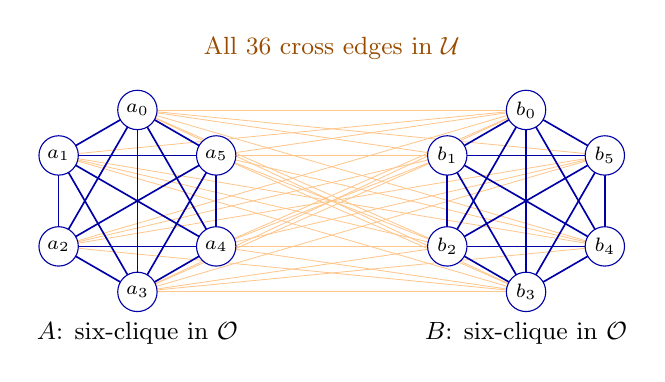
\begin{tikzpicture}[scale=1.05,
 dot/.style={circle,draw=blue!65!black,fill=white,inner sep=0pt,
 minimum size=5mm,font=\scriptsize}]
\foreach \i in {0,...,5} {
 \coordinate (a\i) at ({-2.35+1.1*cos(90+60*\i)},{1.1*sin(90+60*\i)});
 \coordinate (b\i) at ({2.35+1.1*cos(90+60*\i)},{1.1*sin(90+60*\i)});
}
\foreach \i in {0,...,5} \foreach \j in {0,...,5}
 \draw[orange!45,line width=.3pt] (a\i)--(b\j);
\foreach \i in {0,...,5} \foreach \j in {0,...,5} {
 \ifnum\i<\j
  \draw[blue!65!black,line width=.6pt] (a\i)--(a\j);
  \draw[blue!65!black,line width=.6pt] (b\i)--(b\j);
 \fi
}
\foreach \i in {0,...,5} {
 \node[dot] at (a\i) {$a_{\i}$};
 \node[dot] at (b\i) {$b_{\i}$};
}
\node[font=\small] at (-2.35,-1.6) {$A$: six-clique in $\mathcal O$};
\node[font=\small] at (2.35,-1.6) {$B$: six-clique in $\mathcal O$};
\node[font=\small,text=orange!60!black] at (0,1.85) {All $36$ cross edges in $\mathcal U$};
\end{tikzpicture}
\caption{Two further mutually unbiased bases would require twelve
distinct vector-ball labels: six pairwise orthogonality-compatible labels
in each set, with every cross pair unbiasedness-compatible. The graphs
retain all necessary edges. A completed search excluding this pattern
therefore excludes the two bases throughout the phase ball.}
\label{fig:two-cliques}
\end{figure}


\begin{lemma}[Complete graph search]
\label{exclude:graph-search}
The mode-$1$ search of \texttt{graph::exist}, started with both pools
equal to the full vertex set and first-clique target size six, returns
false only if \eqref{exclude:graph-configuration} is impossible.
A work-cap exhaustion never gives a negative certificate.
\end{lemma}
\begin{proof}
First consider \texttt{clique} on a candidate set $P$ and target size
$m$.  For $m=0$ it succeeds, and for $m=1$ it tests nonemptiness.
For $m\ge2$, it repeatedly selects the least remaining vertex $i$,
removes it from $P$, and searches $P\cap N_{\mathcal O}(i)$ for an
$(m-1)$-clique.  For $m=2$ that search is just nonemptiness.
Every clique has a unique least vertex, so this enumerates every
possibility.  Terminating when fewer than $m$ candidates remain is
also exact.

Now suppose that $A,B$ satisfy \eqref{exclude:graph-configuration}.
Interchange their names if necessary so that
$a=\min(A\cup B)$ belongs to $A$.
At the root, \texttt{exist} tries possible least vertices of the
first clique in increasing order.  It deletes each tried root vertex
from both its local first pool and its second pool.  Thus when $a$
is selected, every required remaining vertex in $A\cup B$ is still
available.  This root deletion imposes only the chosen convention
that the minimum of the union lies in the first clique.  It is
performed only when the remaining first-clique target is six,
and therefore not in any recursive call.

After an increasing prefix $S\subseteq A$ has been selected, with
$1\le|S|\le5$, the recursive first pool is the set of vertices larger
than $\max S$ that are $\mathcal O$-adjacent to every vertex of $S$.
The second pool is the set of vertices larger than $a$ that are
$\mathcal U$-adjacent to every vertex of $S$.
Selecting the next vertex $i$ intersects the remaining first pool
with $N_{\mathcal O}(i)$ and the second pool with
$N_{\mathcal U}(i)$.  In the branch selecting the next member of $A$,
these pools still contain the required remaining members of $A$ and
all of $B$, respectively.
The lack of $\mathcal U$ self-loops also removes every selected
first-clique vertex from the second pool.

A first-pool cardinality check cannot reject a pool containing the
needed remaining vertices.  A second-pool cardinality check cannot
reject a pool containing $B$.
The mode-$1$ prune runs the exact auxiliary six-clique test on the
second pool: it too must succeed if $B$ is present, and later
intersections can only shrink that pool.  On selection of the sixth
first-clique vertex, an auxiliary six-clique test of the resulting
second pool is exactly the remaining requirement.
Hence a complete branch survives for every configuration
\eqref{exclude:graph-configuration}.

Finally, all recursive tests interpret exhaustion of the work budget
as possibility and set a persistent give-up flag.  The public
\texttt{candidate} result is the logical disjunction of its search
result and this flag.  A negative result therefore requires both
an exhausted combinatorial search with no configuration and an unset
give-up flag; hitting the cap cannot certify exclusion.
\end{proof}

The graph has at most $2048$ vertices and is represented by $32$
unsigned 64-bit words per adjacency set.  Only valid vertex indices
are inserted, all unused bits are zero, and intersections and
cardinalities are exact integer operations.  A least-set-bit operation
is called only on a nonempty set.  Thus the finite-set operations in
the preceding proof are the operations performed by the code.
The specified search uses mode $1$ and a cap of $5{,}000{,}000$ steps.

\begin{proposition}[Local exclusion certificate]
\label{exclude:local-certificate}
Assume the root certificate
\eqref{exclude:root-data}--\eqref{exclude:root-decomposition} and the
arithmetic guarantees of Section~\ref{sec:rounding}.
If Stage C returns a negative result for the Record, then no exact
Hadamard $e(P+\delta)$ in its closed horizontal radius-$r$ ball can
be extended, together with the coordinate basis, by two further
mutually unbiased orthonormal bases.
\end{proposition}
\begin{proof}
Every additional vector belongs to a bin at the initial resolution.
The necessary tests retain a bin path containing it at all four
resolutions.  If the retained set becomes empty, no such vector
exists.  Otherwise a successful clustering covers all retained bins
by closed balls.  Two additional bases would give twelve distinct
ball labels with every required edge retained, hence a configuration
\eqref{exclude:graph-configuration}.  A completed negative graph
search excludes that configuration by
Lemma~\ref{exclude:graph-search}.
Overflow, clustering failure, a surviving graph possibility, and
work-cap exhaustion are all unresolved outcomes and are never
reported as negative.  These are exactly the two successful negative
paths of \texttt{negative}: an empty completed bin layer, or a
completed negative graph search.
\end{proof}

\subsection{Conservative arithmetic and invocation}
\label{exclude:implementation}

We finish by specifying the outward replacements and comparison margins
that connect the necessary inequalities to the implemented certificate.
Their arithmetic justification is in Sections~\ref{round:single}
and~\ref{round:joint}.

For a bin the source forms its halfwidth with a $10^{-12}$ increase,
then increases each of $X_M,L_M,I_M$ by a further $10^{-12}$ after
the indicated multiplication.  The stored tangent and normal bounds
are formed as
\[
 \widehat r_H=\sqrt{1+\omega}\,r+10^{-9},\qquad
 \widehat n=n_0+\iota r+\Gamma r^2+10^{-9}.
\]
The upper scalar squared-magnitude threshold in
\eqref{exclude:direct-tests} is increased by $2\cdot10^{-7}$,
and its lower threshold, when $\tau<1$, is decreased by that amount.
The combined squared-distance threshold, the right side of
\eqref{exclude:scalar-linear}, and the right side of
\eqref{exclude:bin-support} each receive a $2\cdot10^{-7}$ comparison
allowance.

For a pair, the radius sum is increased by $10^{-10}$.
The distance tests \eqref{exclude:edge-distance} permit a further
$2\cdot10^{-7}$ on that radius.  Both edge residual bounds
$E_{\mathcal O}$ and $E_{\mathcal U}$ are increased by $2\cdot10^{-8}$;
the direct comparisons \eqref{exclude:orth-support} and
\eqref{exclude:unbiased-support} receive another $2\cdot10^{-7}$.
The right side of the joint comparison
\eqref{exclude:joint-inequality} receives $3\cdot10^{-7}$.
Cluster assignment radii include the $10^{-9}$ allowance already
described in Lemma~\ref{exclude:cluster-cover}.

The bounds $|P_{ij}|\le4$ and $|v_j|\le2$ keep all trigonometric
arguments used here within the guarded range of \texttt{expair}.
The proof of Section~\ref{sec:rounding} includes the errors in these
arguments, in $q,S,c,J,B$, in the short weighted sums and norms, and in
the positive support expressions.  Inexact solution of the proposal
systems supplies no separate assumption.

For clarity, the invocation parameters used for this certificate are
\texttt{12 4 1 .042 1 1 5000000}: initial resolution $12$, four bin
layers, one proposed bin direction, clustering parameter $.042$,
one proposed joint direction, graph mode $1$, and the stated graph
work cap.  The two Lloyd iterations are the fixed default.
The conclusion of Proposition~\ref{exclude:local-certificate} is
conditional on a completed negative result for the individual Record;
no collection of unexecuted tests is itself such a result.

\section{Finite execution and the recorded certificate}
\label{sec:execution}

The computation used below was completed on 4 October 2026 (UTC). This
section specifies its finite inputs, the tests for complete execution,
and the implication from those tests to nonexistence. The geometric and
arithmetic justification of each rejection is given in
Sections~\ref{sec:seed}--\ref{sec:exclusion} and
Appendix~\ref{sec:rounding}. A successful exit by itself is not the
certificate: the inputs, record counts, saved failures, and coverage of
all shards must agree as described here.

\subsection{Programs, records, and machine arithmetic}
\label{execute:programs}

The accompanying \texttt{verification/code/} directory contains the seven unchanged
source files \texttt{seed.cpp}, \texttt{covout.cpp}, \texttt{ub.cpp},
\texttt{patchx.cpp}, \texttt{atlas.cpp}, \texttt{stageB.cpp}, and
\texttt{stageC.cpp}. Their byte lengths and full SHA-256 digests are
listed in \texttt{verification/code/extraction.json}. The source hashes were checked
before the recorded run, and the packaged copies match those same bytes.
Only four translation units are
built as entry points:
\begin{center}
\begin{tabular}{lll}
\toprule
Executable & Translation unit & Role\\
\midrule
\texttt{covrun} & \texttt{covout.cpp} & Nine-phase seed cover\\
\texttt{arun} & \texttt{atlas.cpp} & Completion search and coarse atlas\\
\texttt{brun} & \texttt{stageB.cpp} & Certified refinement\\
\texttt{crun} & \texttt{stageC.cpp} & Vector cover and graph exclusion\\
\bottomrule
\end{tabular}
\end{center}
The other files are included through the macros in these translation
units. Their standalone sample drivers are not executed. In particular,
A uses \texttt{Asearch}, and C uses graph search mode~1.

A serialized \texttt{Record} contains a certified \texttt{Root} and a
radius $r$. Its interpretation is the set of exact Hadamard solutions
represented, up to the equivalences of Section~\ref{sec:seed}, by
$e(p+h)$ with horizontal $h$ and $\|h\|\le r$. The stored $p$ need not
itself be an exact solution. The Root data justify the normal-displacement
inequalities on this set; their construction is part of
Section~\ref{sec:phase-cover}.

The binary format is explicit. A file begins with an eight-byte unsigned
record count. Each record consists, in order, of a four-byte signed
integer $k$, 36 binary64 entries of $p$, $k$ rows of 36 binary64 entries
of $T$, and the eight binary64 values
\[
 C,\ n_0,\ \mathrm{id},\ \mathrm{ort},\ \mathrm{hor},\
 \mathrm{mnorm},\ \mathrm{froot},\ r.
\]
Thus a record occupies $356+288k$ bytes, and a valid zero-count file is
exactly eight bytes. The platform is little endian. No phase data are
converted to decimal between stages. The evidence checks parse every
record, validate finite bounded fields, and require the declared count
to reach the exact end of file. They also check that every saved C
failure is an unchanged, ordered subsequence of its assigned inputs.

The recorded platform was x86-64, Intel Xeon Platinum 8573C, Ubuntu
GCC 13.3.0, and glibc 2.39. The builds, prepared on the same UTC date
before the run, were
\begin{lstlisting}
g++ -O3 -march=native -ffp-contract=off covout.cpp -o covrun
g++ -std=gnu++17 -O3 -march=native -ffp-contract=off atlas.cpp -o arun
g++ -std=gnu++17 -O3 -march=native -ffp-contract=off stageB.cpp -o brun
g++ -std=gnu++17 -O3 -march=native -ffp-contract=off stageC.cpp -o crun
\end{lstlisting}
The first command used this compiler's default GNU C++17 dialect.
The arithmetic assumptions are binary64, round to nearest, separate
operations without contraction or fast-math reassociation, correctly
rounded binary64 square root, masked floating-point exceptions, and
neither flush-to-zero nor denormals-are-zero. Separate probes compiled
with the cover and A/B/C flag sets both passed and recorded
\texttt{FLT\_EVAL\_METHOD=0}, 32-bit \texttt{int}, 64-bit
\texttt{size\_t}, 64-bit \texttt{uint64\_t} equal to
\texttt{unsigned long}, eight-bit bytes, and MXCSR \texttt{0x1f80}.
Both probes recorded nearest rounding on entry and during the check,
and passed the square-root and gradual-underflow samples. These probes
and the program checks provide limited evidence for the stated platform
conditions, not a proof of all primitive-operation or compiler semantics.
Those semantics remain assumptions; Appendix~\ref{sec:rounding} supplies
the numerical bounds under them. The retained
\texttt{build/build-manifest.json} identifies the exact sources,
binaries, compiler commands, probe outputs, and arithmetic evidence.

One additional code-generation condition is needed by
\texttt{coverSeeds::run}: both \texttt{pow(\ldots,2)} expressions must
be lowered to the binary64 multiplications analyzed in
Appendix~\ref{sec:rounding}. For the actual \texttt{covrun}, inspection
of the saved disassembly finds the scale multiplication, its square,
subtraction, square root, addition, and second square at hexadecimal
addresses \texttt{6035}, \texttt{6039}, \texttt{603d},
\texttt{605c}, \texttt{606d}, and \texttt{608b}, respectively. There
is no dynamic \texttt{pow} symbol. Absence of that symbol alone would
not establish the required instruction sequence. The recorded binary is
identified by its full SHA-256 digest, so this check applies to that build.
The specified lowerings address only this code-generation condition, not
the full arithmetic model itself. A new build requires
this check again. Its binary hash, like any native build hash, need not
equal that of the recorded binary.

\subsection{Specified finite control flow}
\label{execute:control}

All invocations use the C numeric locale and fresh output paths.
The cover is run to normal completion before A reads its output.
A uses all four parts $i=0,1,2,3$ with \texttt{parts=4}; part $i$
processes exactly the center indices congruent to $i$ modulo~4.
Its constants are seed radius \texttt{.0320001}, local target
\texttt{.103}, global target \texttt{.125},
\texttt{levels=3}, \texttt{iters=2}, and \texttt{first=1}.

The following are the program invocations, with $i$ and $j$ standing for
the indicated shard and batch indices. The accompanying
\texttt{verification/code/proof\_run.py} runner was used in this execution and
performs the validation between stages; this display only specifies the
program arguments. A separate bounded supervisor retained the runner's
exit and process-cleanup record.
\begin{lstlisting}
export LC_ALL=C
./covrun centers.txt
./arun centers.txt i 4 coarsei.bin badi.txt
./brun .07 .013 mid.bin midbad.bin - \
  coarse0.bin coarse1.bin coarse2.bin coarse3.bin
./brun .016 .005 fine.bin finebad.bin batches/f mid.bin
./crun 12 4 1 .042 1 1 5000000 0 1 \
  batches/badj.bin batches/fj.bin
./brun .011 .0038 fb1.bin fb1bad.bin - ALL_NONEMPTY_C_BAD_FILES
./crun 12 4 1 .042 1 1 5000000 i 4 fb1cbadi.bin fb1.bin
\end{lstlisting}
There is one initial C invocation for every batch named by the completed
\texttt{batches/fdone.txt} marker. In C the first seven parameters mean
initial grid $12$, four layers, one linear-support iteration, proposed
cluster radius $.042$, detail~1, graph mode~1, and graph-step cap
$5{,}000{,}000$. Thus the single-vector grids are $12,24,48,96$.
The unchanged default number of clustering passes is two.

The mid and fine B invocations are sequential. A batching B invocation
writes consecutive groups of at most 256 atlas records, replacing each
batch radius by its target $.016$, and atomically renames each completed
batch. The checked concatenation of all batch records equals
\texttt{fine.bin}, except for that radius replacement. Every original
fine radius is at most $.016$, so the replacement enlarges the represented
sets. The completion marker agrees with both the number of batches and
the sum of their record counts. The recorded run waited for B fine to
finish before starting C; it used up to sixteen independent C workers.
Concurrency changes scheduling only: workers have distinct output files
and do not share mutable search state.

For every initial C process, the normal status is 0 exactly when its
saved bad count is zero, and 1 exactly when that count is positive.
The four reported failure categories---uncapped graph candidate,
graph-step cap, bin overflow, and clustering failure---sum to that bad
count. None of them is an exclusion. Every nonempty-count bad file is
passed to B fallback in C-locale filename order, including failures whose
locations differ from those in another run. Final C uses all four
modulo-4 parts of the fallback output. If initial C has no bad records,
fallback and final C are unnecessary; that shortcut was not used in the
recorded run.

The required terminal conditions are:
\begin{enumerate}
\item successful builds, a normally completed cover, and a complete
      center file;
\item four A exits 0, all assigned centers processed, terminal
      \texttt{failedBalls=0}, and four empty bad text files;
\item both B exits 0, all input parents processed, agreement of logged
      and saved output counts, and zero-count B bad files;
\item every initial C batch processed exactly once with consistent
      exit, done count, bad count, and saved records;
\item every initial C bad record included in fallback, fallback exit 0
      with all parents processed and zero saved failures, and four
      final C exits 0 with total done equal to the fallback count and
      zero saved failures.
\end{enumerate}
Missing files, truncated data, an unexpected exit, resource exhaustion,
an unresolved A or B parent, or a final C bad record prevent acceptance.
Recoverable search diagnostics are distinguished from these terminal
conditions. For example, A's \texttt{ownfail} counts unsuccessful
proposals of a local Root cover that are followed by subdivision. A0
reported such a diagnostic in this run; its terminal unresolved count
was nevertheless zero.

\subsection{Finite bounds and conservative stopping}
\label{execute:bounds}

The control flow has explicit finite bounds. Before filtering, the
nondecreasing five-bin lists for the seed cover number at most
\[
 \binom{116}{5}=160{,}389{,}488,
\]
and for any fixed shared bin the four ordered tail bins number at most
\[
 \binom{115}{4}=6{,}913{,}340.
\]
The former bound is below the signed 32-bit limit. Pair traversals use
range loops and 64-bit counters. All bin differences lie between $-111$
and $111$; their nine-coordinate square sum is at most $9\cdot111^2$,
so the integer distance and bucket arithmetic fit the stated types.
The stored five-coordinate differences also fit the signed eight-bit
type used by the cover.

A retains nonfinal unitary grid lists only through grid~32; the grid~64
has at most $64^4/8=2{,}097{,}152$ cell tests per seed. Further tests
are bounded by the $1{,}000{,}000$ extra-node cap, and the deepest
grid is 512. Reaching the cap or reaching the deepest grid without a
certificate records an unresolved seed. Trial-direction and Root
proposal failures can lose an opportunity to cover a cell, but cannot
make an uncovered cell successful. The local candidate list uses
\texttt{topK=4} in an array of size~8.

The Root dimension is at most $k=10$. Atlas sizes and individual record
file counts are capped at $2{,}000{,}000$, and concatenated B/C input
counts at $8{,}000{,}000$. For B the validated widths and radii give
$L\le1262$ and hence axis indices at most 2524; the product grid is
checked against $50{,}000{,}000$ before multiplication. Mixed-radix
strides and marks therefore fit the stated index types. Each unresolved
box is split to depth at most six, and the $2^k$ child masks fit an
integer. Only successfully completed parents are inserted into B's
list of earlier covered parents. A grid-cap rejection is a parent
failure, not a completed parent.

C retains at most $2{,}000{,}000$ phase bins. The first grid has
$12^5=248{,}832$ cells; a later grid tests at most 32 children per
retained bin. Clustering permits at most 2048 balls. Its graph bitsets
have 32 words of 64 bits, and all members have indices below the current
node count. Word shifts are unsigned. The graph pair counts fit an
integer, and the joint test has at most 14 rows. Recursive clique
search decreases the requested clique size or removes a candidate;
the step cap supplies an additional bound. A cap sets the conservative
candidate/give-up flag and saves the record. It does not return a
negative certificate. Consequently no finite resource cap in the
specified run can establish nonexistence by silently dropping a region.

\subsection{The finite-execution implication}
\label{execute:implication}

\begin{theorem}[Finite-execution certificate]
\label{execute:finite-theorem}
Use the seven specified source files and the arithmetic conditions of
Appendix~\ref{sec:rounding}. Suppose the invocations in
Section~\ref{execute:control} meet all of its terminal conditions, with
the record provenance and batch checks stated there. Then four mutually
unbiased orthonormal bases in $\C^6$ do not exist.
\end{theorem}

\begin{proof}
Suppose four such bases exist. Normalize the first to the standard basis
and write the second as $H/\sqrt6$. Proposition~\ref{seed:cover} places
the seed coordinates of an equivalent exact Hadamard matrix in one of
the generated seed balls. All A shards together process that seed.
Proposition~\ref{phase:A-cover} therefore places an equivalent exact
solution in a coarse Record. Each equivalence preserves extendibility
by two further bases.

Apply Proposition~\ref{refine:cover-preservation} first to B mid and
then to B fine, and Corollary~\ref{refine:batch-cover} to the emitted
batches. They place
an equivalent exact solution in a record of \texttt{fine.bin}, and
therefore in its checked, possibly enlarged batch record. Completeness
of the marker and the per-batch done counts ensures that initial C
processes that record. A negative C result would contradict its
extendibility by Proposition~\ref{exclude:local-certificate}. Hence it
must occur among the saved initial failures. If there are none, this
already gives a contradiction. Otherwise the fallback branch is executed,
and the subsequence and fallback-input checks include that very record
in B fallback.

The successful fallback again covers its exact solutions, up to the
same equivalences, by the records of \texttt{fb1.bin}. The final four
modulo-4 shards partition those records without omission. Every final
record has a negative C result, contradicting extendibility. Each
coverage implication used here is justified by its geometric lemma and
the one-sided arithmetic bounds; counts and hashes establish the
identity and completeness of the finite chain, not those inequalities
in isolation.
\end{proof}

\subsection{The completed execution}
\label{execute:observed}

The execution began at 03:10:26 and completed at 04:24:56 on
4 October 2026 (UTC). Both the runner and its supervisor exited 0;
the supervisor recorded no cleanup or finalization errors, no remaining
children, and unchanged input hashes. The execution evidence includes
the raw command and stream records, exact file contents, record provenance,
batch concatenation, actual fallback inputs, and final modulo partition.
Together with the validation records, these account for all 100 native
invocations and show no final unresolved records. They document the finite
execution, not an automatic verification of the geometric or arithmetic
lemmas.

Table~\ref{execute:counts} records this computation. All four A shards exited 0,
with empty bad text files. Each B invocation exited 0 with an eight-byte
zero-count bad file. Initial C had 73 exits 0 and 15 exits 1, all
accounted for by saved failures. All final C shards exited 0 with
eight-byte zero-count bad files.

\begin{table}[htbp]
\centering
\small
\begin{tabular}{lrrl}
\toprule
Stage & Inputs processed & Output records & Unresolved records\\
\midrule
Seed cover & $151{,}744{,}086$ pairs & $249{,}878$ centers & ---\\
A0 & $62{,}470$ & 764 & 0\\
A1 & $62{,}470$ & 774 & 0\\
A2 & $62{,}469$ & 757 & 0\\
A3 & $62{,}469$ & 788 & 0\\
B mid & 3083 & 600 & 0\\
B fine & 600 & $22{,}379$ & 0\\
Initial C & $22{,}379$ & --- & 163 (all graph caps)\\
B fallback & 163 & 1127 & 0\\
Final C0 & 282 & --- & 0\\
Final C1 & 282 & --- & 0\\
Final C2 & 282 & --- & 0\\
Final C3 & 281 & --- & 0\\
\bottomrule
\end{tabular}
\caption{Observed execution on 4 October 2026 (UTC). The seed cover retained
22,829 five-bin $x$ lists. The fine records form 88 batches:
$87\cdot256+107=22{,}379$.}
\label{execute:counts}
\end{table}

The nonzero initial C failure files, in the actual order supplied to
B fallback, were
\begin{lstlisting}
bad10.bin bad3.bin bad4.bin bad5.bin bad52.bin bad53.bin
bad55.bin bad56.bin bad6.bin bad7.bin bad78.bin bad79.bin
bad8.bin bad80.bin bad84.bin
\end{lstlisting}
They contain all 163 unresolved records. There were no initial bin
overflows, clustering failures, or uncapped graph candidates. There
were no final failures of any category. Thus all 100 program invocations
in the full pipeline are accounted for: one cover, four A processes,
two B refinements, 88 initial C processes, one B fallback, and four
final C processes. The fifteen initial C exits 1 are resolved by that
fallback chain. No rejection threshold, graph cap, refinement width,
or mathematical source file was altered, and no additional refinement
level was inserted.

For scale, the wrapper-measured stage wall times, including polling and
validation, were 621.59 seconds for the cover, 2020.32 seconds for the
four parallel A shards, 1071.49 and 407.45 seconds for B mid and B fine,
and 300.23, 8.12, and 36.27 seconds for initial C, fallback B, and final C.
The outer supervisor measured 4470.33 seconds for the complete pipeline.
These are observations on this platform, not native CPU times or
running-time guarantees. No stage hit its wall deadline, and no retry
or resource-limit increase was used.

\begin{longtable}{@{}p{.19\textwidth}p{.77\textwidth}@{}}
\caption{SHA-256 digests of the actual principal data files. Full
per-file inventories accompany the computation archive.}
\label{execute:hashes}\\
\toprule
File & SHA-256\\
\midrule
\endfirsthead
\toprule
File & SHA-256\\
\midrule
\endhead
\texttt{centers.txt} & {\scriptsize\texttt{c48bc9a2be1eb2cdeea82ea1b030d7cb9f00a6c9563b63f0248dd115748a5789}}\\
\texttt{coarse0.bin} & {\scriptsize\texttt{77b0cda59484ffde0654db8d6008bcaab1daf1deefd00d4dc085d3d751418cd4}}\\
\texttt{coarse1.bin} & {\scriptsize\texttt{48ca7775dba57a87a10d154da8b172074b29c9a65b32e44ee169f23a48d24b8a}}\\
\texttt{coarse2.bin} & {\scriptsize\texttt{418b6d9cf338187c63635d26050940a13177515050a057b2bc67fd11a163e43e}}\\
\texttt{coarse3.bin} & {\scriptsize\texttt{8c23427e63e31cd18abbb80838e3289e646fd108fa850687ca7b857471376535}}\\
\texttt{mid.bin} & {\scriptsize\texttt{e97c74dde90a0e758df2cb5d9708f5bd6bd660ed920b3299f5df92ff4de11be4}}\\
\texttt{fine.bin} & {\scriptsize\texttt{9b5b743b61907277fa6687a0ad45677bbcd0e4c9bd44a0d93d258253fb52923d}}\\
\texttt{fb1.bin} & {\scriptsize\texttt{ef85ec73217ecb0c770d3c775396df88b60ca06918f77310df5dff2f6d9bf215}}\\
\bottomrule
\end{longtable}

The execution archive identified by
\texttt{verification/\allowbreak computation/README.md} preserves the numerical data and records
of this complete run, with internal path and host fields redacted: all sources
and binaries, center and record files, all 88 input batches and their C
bad files, fallback data, all final bad files, stdout and stderr,
commands, exits, platform information, and validation records. In the
execution archive, \texttt{full-run-01/pipeline/status.json} is the
whole-run record; \texttt{*.stage.json} files describe stages and
individual \texttt{*.status.json} files describe child processes.
The outer record is \texttt{full-run-01/run.json}.
\texttt{verification/REPRODUCE.md} gives rebuild and
execution instructions. Archived native binaries document this run;
they are not a portability claim.

The proof here uses only this newly completed chain and the values in
Tables~\ref{execute:counts} and~\ref{execute:hashes}. The complete
evidence packet for the execution reported on 7 September 2026 was not
recovered. Although the new principal data hashes and stage counts agree
with those reported for that run, this agreement does not authenticate
the earlier execution. Neither its reported results nor earlier timed
or sampled diagnostics substitute for any stage of the new full run.

\section{Conclusion of the proof}\label{sec:conclusion}

\begin{proof}[Proof of \cref{thm:main}]
Under the arithmetic and compiler conditions specified in
Section~\ref{execute:programs} and Appendix~\ref{sec:rounding}, the
checked terminal, provenance, and batch data for the execution
documented in Section~\ref{execute:observed} permit application of
Theorem~\ref{execute:finite-theorem}. It excludes four mutually unbiased orthonormal bases in
$\C^6$. Lemma~\ref{lem:three-mub-six} gives three such bases, so
$N(6)=3$.
\end{proof}


\appendix
\section{Certified arithmetic}\label{sec:rounding}

This section supplies the one-sided arithmetic estimates used in
Sections~\ref{sec:seed}, \ref{sec:completion}, \ref{sec:phase-cover},
\ref{sec:refinement}, and~\ref{sec:exclusion}.
The source files, parameters, build, and completed execution are
documented in Section~\ref{sec:execution}.  The estimates concern those entry points
and parameters.  Auxiliary routines not called by those entry points are
not additional exclusion tests.

We distinguish an \emph{exact stored number}, meaning the real number
represented by a binary64 datum, from the ideal mathematical quantity it
approximates.  Proposed solve directions, proposed inverse matrices, and
proposed changes of basis are usually used in the first sense.  Their
accuracy is not assumed: finite bounds and residual inequalities are
checked before a proposal can justify an exclusion or a covering step.
For complex arrays, an entrywise error is an error in complex modulus.
Matrix norms without a subscript are Euclidean operator norms.

\subsection{Arithmetic premises and elementary estimates}
\label{round:premises}

The primitive-operation model is the binary64 specification of
IEEE~754~\cite[Sections~3.4, 3.6, 4.3, 5.4.1 and~7.5]{IEEE7542019}.
The accumulation estimates use the usual product-of-rounding-factors
argument~\cite[Section~2.12 and Lemma~3.1]{Higham2002Accuracy}, with the
explicit additive underflow allowance retained below.

The arithmetic premises are separate, correctly rounded binary64
addition, subtraction, multiplication, division, and square root in
round-to-nearest mode, with binary64 evaluation of intermediate results.
The build uses \texttt{-ffp-contract=off}, and does not use fast-math or
reassociation that changes these operations.  Subnormal numbers are not
flushed to zero, and denormal inputs are not treated as zero.  Floating
exceptions are masked, so an unsuccessful heuristic calculation can
produce an infinity or NaN and be rejected by its subsequent checks.
The relevant integer types, numeric locale, and file representation are
specified in Section~\ref{sec:execution}.

The function \texttt{environment} sets and checks nearest rounding and
checks the binary64 properties of \texttt{double}.  The A/B/C entry points
also inspect MXCSR, rejecting a non-nearest mode, DAZ, FTZ, or unmasked
exceptions.  The same no-DAZ/no-FTZ environment is required for
\texttt{covout}, although its entry point does not itself inspect those
bits.  The default-nearest premise also applies to constants and the
global basis constructed before \texttt{main}.  These are explicit
arithmetic premises, not a claim that a source-level static assertion
formally verifies every compiler transformation.  The recorded build
checks and their limits are described in Section~\ref{sec:execution}.

The functions \texttt{nearbyint} and \texttt{floor} choose integers at
finite bounded arguments.  The particular integer chosen at a boundary
is permissible wherever the proof subsequently uses that integer lift.
No accuracy premise is imposed on \texttt{atan2}: Candidate checks the
unit exponential of the phase it proposes.  Decimal literals are either
used as exact stored parameters, or allowed a relative translation error
of at most $5\cdot10^{-16}$ when compared with a displayed decimal.

Put
\begin{equation}\label{round:unit}
 u=2\cdot10^{-16},\qquad \tau=10^{-300},\qquad
 \gamma_m=2.1\cdot10^{-16}(m+1).
\end{equation}
For a correctly rounded basic operation with finite exact result $z$ at
the scales below,
\begin{equation}\label{round:basic}
 |\operatorname{fl}(z)-z|\le u|z|+\tau.
\end{equation}
The true binary64 relative unit roundoff is smaller than $u$, and the
additive allowance is much larger than half the least positive
subnormal.  Overflows are excluded for the certificate evaluations by
the scale bounds proved below; they need not be excluded in an
untrusted solve.

\begin{lemma}[Accumulation and norm bounds]\label{round:accumulation}
For $m\le2000$, a dot product on exact stored inputs, formed as separate
products and successive additions, satisfies
\begin{equation}\label{round:dot}
 \left|\operatorname{fl}\!\left(\sum_{i=1}^m a_i b_i\right)
                  -\sum_{i=1}^m a_i b_i\right|
 \le \gamma_m\sum_{i=1}^m|a_i b_i|+4(m+1)\tau.
\end{equation}
An initial addend is included in the absolute sum and increases the
small operation-count constant by one.  A product of three factors
instead of two increases that constant by one more.
For the square-sum/square-root norms used here,
\begin{equation}\label{round:norm}
 \left|\operatorname{fl}(\|a\|)-\|a\|\right|
 \le 2.2\cdot10^{-16}(m+2)\|a\|+10^{-140}.
\end{equation}
If the computed components approximate other components, their
Euclidean difference is added to this bound.
\end{lemma}

\begin{proof}
For each product term, the product rounding and the additions through
which it passes contribute at most $m+1$ multiplicative factors of the
form $1+\delta$, $|\delta|\le u$.  In the stated range,
$(1+u)^{m+1}-1<\gamma_m$.  Propagating the additive errors in
\eqref{round:basic} costs less than $4(m+1)\tau$; all amplification
factors here are less than $1.001$.  This proves \eqref{round:dot}.
The same argument applies to positive sums and to three-factor products.
For a sum of squares it gives relative error at most $\gamma_m$ and an
additive error at most $4(m+1)\tau$.  Taking its square root, using
$|\sqrt{1+t}-1|\le |t|/(1+\sqrt{1-|t|})$ for $|t|<1$, and then including
the final square-root rounding gives \eqref{round:norm}.  The additive
effect is bounded by $\sqrt{4(m+1)\tau}$ plus the square-root rounding;
this is smaller than $10^{-140}$.  Finally
$|\|a\|-\|b\||\le\|a-b\|$.  Thus no division by a small norm is needed
to handle perturbed components.
\end{proof}

For exact stored complex numbers, the explicit source operations obey
\begin{align}
 |\operatorname{fl}(z+w)-(z+w)|
   &\le u(|z|+|w|)+2\tau,\label{round:complex-add}\\
 |\operatorname{fl}(zw)-zw|
   &\le 10^{-15}|z||w|+8\tau.\label{round:complex-multiply}
\end{align}
For the latter, each real component uses two real products and an
addition or subtraction.  Its error is bounded by
$(2u+u^2)$ times the sum of the two absolute products, plus the additive
allowance.  Cauchy's inequality bounds each such sum by $|z||w|$, and
$\sqrt2(2u+u^2)<10^{-15}$.  Real scaling and division are componentwise
instances of \eqref{round:basic}.  Squared moduli also satisfy the useful
perturbation bound
\begin{equation}\label{round:squared-perturbation}
 \big||z+e|^2-|z|^2\big|\le2|z||e|+|e|^2,
\end{equation}
before their own multiplication/addition errors.

The additive underflow terms can be retained throughout these
inequalities.  The norm allowance $10^{-140}$ is deliberately loose.
All subsequent certified divisions have the explicit lower bounds
given below; in particular the residual test divides only by a gap
of order $10^{-6}$ or larger.  Its norm factors and scale are at most
the displayed $10^8$--$10^{11}$ scales, so its propagated additive
terms remain below $10^{-120}$.  The second square root in the spectral
estimate is handled separately by an absolute term of order
$10^{-69}$.  That term is covered there before the result is reused.
Other normalizations have denominators bounded below by $.148$, $.45$,
or larger.  At each iterative upper-bound update the new local error is
absorbed by its own positive margin.  There is therefore no unchecked
chain of ill-conditioned divisions propagating a subnormal error: all
such additive contributions are below $10^{-50}$ when they are
absorbed in the strict budgets below.

\subsection{Pi and unit exponentials}
\label{round:exponentials}

The source literal \texttt{0x1.921fb54442d18p+1} represents the
binary rational
\[
 \widehat\pi=\frac{884279719003555}{281474976710656}.
\]
Here is an exact certificate for its error.  Write
\[
 A(x,n)=\sum_{j=0}^{n-1}\frac{(-1)^j x^{2j+1}}{2j+1},\qquad
 s=16A(1/5,12)-4A(1/239,4).
\]
If $t=\arctan(1/5)$, then $\tan(2t)=5/12$ and
$\tan(4t)=120/119$; subtracting $\arctan(1/239)$ gives tangent $1$
in $(0,\pi/2)$.  This proves Machin's identity
$\pi=16\arctan(1/5)-4\arctan(1/239)$.
The alternating-series remainder gives
\[
 |s-\pi|\le \frac{16}{25\,5^{25}}+\frac{4}{9\,239^9}.
\]
Exact rational arithmetic gives
\begin{equation}\label{round:pi-rational}
 \widehat\pi-s=
 \frac{-1204334632739641172855772829555432415587}
 {10003273510806667494906565283020800000000000000000000000}.
\end{equation}
Adding the displayed rational remainder bounds and comparing integers
proves
\begin{equation}\label{round:pi-error}
 |\widehat\pi-\pi|<1.225418\cdot10^{-16}<2\cdot10^{-16}.
\end{equation}

The range-reduction argument uses Sterbenz's exact-subtraction lemma
\cite{Sterbenz1974FloatingPoint}; a statement including gradual
underflow is given in~\cite[Theorem~2.5 and the following discussion]{Higham2002Accuracy}.
The polynomial and argument-error estimates are proved here for the
particular degree-$18/19$ implementation.

\begin{lemma}[Unit-exponential error]\label{round:expair}
At a finite stored $x$ with $|x|\le16$, \texttt{expair} differs from
$e(x)=\exp(2\pi i x)$ in complex modulus by less than $2\cdot10^{-14}$.
For all its uses in the certificate, including argument formation,
the following common bound is valid:
\begin{equation}\label{round:exp-budget}
 \varepsilon_{\exp}=6\cdot10^{-14}.
\end{equation}
\end{lemma}

\begin{proof}
The multiplication $4x$ is exact.  Let $k$ be its nearest integer.
Then $|x-k/4|\le1/8$.  If $k\ne0$, $x$ and $k/4$ have the same sign
and their absolute values are within a factor two, so the subtraction
is exact by Sterbenz's lemma.  If $k=0$ it is immediate.  Multiplication
by the exact double $2\widehat\pi$ forms a stored angle $y$ with
\[
 |y-2\pi(x-k/4)|<3\cdot10^{-16},\qquad |y|<.786.
\]
The error follows from \eqref{round:pi-error}, the remainder bound $1/8$,
and one multiplication rounding.

The source evaluates cosine through degree 18 and sine through degree
19.  In the $j$th nonconstant term, the error in $-y^2$ is reused $j$
times, and there are $j$ further multiplications and $j$ divisions.
The small integer denominators are exact.  Its relative error is
therefore at most $(1+u)^{3j}-1<5.5\cdot10^{-15}$ for $j\le9$.
For additive underflow errors, compare with a recurrence using the
same multiplicative rounding factors but zero additive errors.
Its terms have magnitude below two, and each recurrence contracts
the previous additive error by a factor less than $1/2$:
the numerator factor has magnitude below $.786^2$ and the smallest
denominator is two.  Errors from that factor, the product, and the
division give the conservative recurrence
$E_j\le E_{j-1}/2+4\tau$, $E_0=0$.
Thus $E_j<8\tau$; after both coordinates' nine additions their
total contribution is below $10^{-295}$, including when $y^2$
or a later term underflows.
The absolute even-term sum at $.786$ is below $1.4$, its nonconstant
part below $.4$; the odd-term sum is below $1$, its part after $y$
below $.2$.  For the nonconstant even terms the successive ratio
after the first is at most $.786^2/12$, and for the odd terms after y
it is at most $.786^2/20$.  Their geometric majorants give the claimed
absolute sums without evaluating a transcendental function.
The first omitted cosine and sine terms
are below $3.330\cdot10^{-21}$ and $1.247\cdot10^{-22}$, respectively;
in particular both tails are below $4\cdot10^{-20}$.

The term errors contribute less than $2.2\cdot10^{-15}$ in cosine and
$1.1\cdot10^{-15}$ in sine.  Put
$\alpha=(1+u)^9-1<1.81\cdot10^{-15}$ and
$\rho=(1+u)^{27}-1<5.5\cdot10^{-15}$.
Including the nine additions and the tails gives coordinate errors
less than
$.4\rho+1.4(1+\rho)\alpha+4\cdot10^{-20}<4.74\cdot10^{-15}$
and
$.2\rho+(1+\rho)\alpha+4\cdot10^{-20}<2.92\cdot10^{-15}$.
Their Euclidean combination, the $3\cdot10^{-16}$ angle error,
and the additive underflow term give complex error below
$6\cdot10^{-15}$, hence below the asserted
$2\cdot10^{-14}$.  The quadrant permutations and sign changes are exact.

For a rational bin midpoint, division by the grid size, or multiplication
of $b+1/2$ by the stored reciprocal of that size, has error below
$5\cdot10^{-16}$ cycles.  The latter product has ideal magnitude at
most one.  Subtraction of a phase of magnitude at most four, or a
stored ball phase of magnitude at most two, brings the total argument
error to less than $2\cdot10^{-15}$ cycles.  The Lipschitz constant of
$e$ is $2\pi$, so this additional error fits inside
\eqref{round:exp-budget}.  Dyadic unitary centers are exact; Stage A
treats the stored seed phases as exact after enlarging the seed ball;
\texttt{buildH} treats its stored $p$ as exact and compares row-edge
exponentials with products of ideal unit entries.
\end{proof}

All relied-on arguments satisfy the range condition.  Seed and dyadic
unitary phases are bounded near $[0,1]$; \texttt{gen} checks $|p_j|\le4$;
Candidate checks $|P_j|\le.51$ before its exponential; C validates
$|p_j|\le4$ and checks ball phases of magnitude at most two.
The largest C difference has magnitude at most six.  The constants
$\sqrt6$ and its reciprocal are formed by the indicated square root
and division; $2\cdot10^{-15}$ is an ample absolute error bound for each.

\subsection{Seed filtering and seed-ball reuse}
\label{round:seed}

Here $n=112$ and the stored $w$ approximates $1/n$.
Midpoint-gap calculations contain only small integer arithmetic and
a few products/subtractions; \eqref{round:basic} bounds their total
error, including the comparison threshold, by $10^{-14}$.
Their slack is $10^{-8}$.  The orientation filter is integral.

For a list of five varying phases, the computed residual $c$ in
\texttt{sumok} has component error below $2\cdot10^{-13}$.
Indeed its five exponential errors, after division by $2\pi$, total
less than $4.8\cdot10^{-14}$ in complex modulus, and the divisions,
additions, and constant error cost less than $3\cdot10^{-15}$.
The sharper componentwise bound $1.1\cdot10^{-13}$ will also be useful.
Each test direction is regarded as an exact stored pair; its norm is
less than $1.1$.  The five column perturbations, the residual
perturbation, and ordinary arithmetic in \texttt{chk} cost together
less than $10^{-11}$.  Its remainder coefficient approximates
$5\pi/(4n^2)$ within $10^{-15}$.  The actual $10^{-8}$ comparison
addition therefore preserves every feasible list.

For \texttt{extend}, the stored direction has norm at most $1.01$.
Let $v$, $a$, and $r$ denote its stored directional residual in grid
units, shared coefficient, and support before inflation.  Their errors
satisfy
\begin{equation}\label{round:clip-errors}
 |\Delta v|<3.3\cdot10^{-11},\qquad
 |\Delta a|<10^{-13},\qquad |\Delta r|<10^{-12}.
\end{equation}
For the first bound, multiply the sharpened residual bound by $112$
and by a direction of norm at most $1.01$, and include a two-term dot
and one multiplication.  The other two follow from
\eqref{round:exp-budget}, four absolute support terms, and a
two-component norm.  If $|d_s|\le1/2$ is feasible, these estimates give
\[
 |v+a d_s|\le r+3.3\cdot10^{-11}
                 +\tfrac12\cdot10^{-13}+10^{-12}+\text{rounding}.
\]
The source adds $10^{-7}$ to $r$ \emph{before} dividing by $|a|$.
It skips $|a|<10^{-6}$; at an accepted divisor
$|a|>.999\cdot10^{-6}$, allowing literal translation.
The midpoint quotient has magnitude below $1.2\cdot10^8$ and the
radius quotient below $3\cdot10^6$: the residual has magnitude below
112, and the support before division is below three.  Their divisions
and endpoint additions can move an endpoint by less than $10^{-7}$.
The extra $10^{-5}$ on each endpoint is therefore sufficient.
Intersecting these outward intervals retains the true shared value.

In \texttt{supdual}, all proposed entries are checked by
$|v_a|\le10^4$, with a negated comparison that also rejects NaN.
They are then exact stored test coefficients.  The four right-hand
side errors against $-nc$ are below $3\cdot10^{-11}$ each.  The signed
term consequently has input error at most
\[
 2\sum_{a=1}^4 |v_a|\,3\cdot10^{-11}
 \le2.4\cdot10^{-6}<2.5\cdot10^{-6}.
\]
Its absolute term sum is below $10^7$, so its arithmetic error is below
$10^{-7}$.  Each of the nine row-dot residuals has error below
$4\cdot10^{-9}$: its four input contributions are at most
$4\cdot10^4\varepsilon_{\exp}$, and its short dot costs less than
$10^{-10}$.  Each pair norm has error below $10^{-10}$ by
\eqref{round:norm}.  The remainder coefficient uses $1.251$ instead
of $1.25$, which leaves positive slack after its own rounding.
The final absolute scale is below $2\cdot10^7$.  Summing these
contributions shows that the ideal support expression is at most the
computed proposal plus $10^{-4}$.  The actual addition is $.01$.
If no usable proposal improves the initial $10^{10}$ bound, that
initial bound already exceeds the trivial support.

Integer differences lie in $[-111,111]$, including those stored in
\texttt{int8\_t}; all their squared/absolute sums are exact and small.
The comparison radius is
\[
 \texttt{RN2}=\operatorname{fl}((\operatorname{fl}(.032\cdot112))^2)
              -.0001
\]
with the source's indicated operation ordering.  The total possible
error before the subtraction is below $10^{-12}$, so this is smaller
than the ideal $(.032\cdot112)^2$.  This reasoning requires the
\texttt{pow(x,2)} calls in \texttt{covout} to be lowered to binary64
multiplication, as checked for the fresh build documented in
Section~\ref{sec:execution}.  It is not a claim about an arbitrary
library implementation of \texttt{pow}.  The other square-power value
$T$, bucket reach, and integer cuts only select reuse attempts; missing
an attempt does not discard the current bin pair.  A newly inserted
midpoint needs radius only $1.5/112<.032$.  Finally, the nine
division-rounded seed phases differ from their rational midpoints in
norm by less than $10^{-14}$, which is absorbed when the A seed radius
is increased to $.0320001$.

\subsection{Frames, comparison blocks, and A exclusion tests}
\label{round:frames}

All ideal quantities in this subsection use exact unit exponentials
at the specified centers, and the same coordinate indices selected by
the code.  We never need the selected coordinate to maximize the
\emph{ideal} projection score.

For \texttt{frame}, the four-term sum $S$ has error below
$2.5\cdot10^{-13}$; its squared modulus has error below
$2.2\cdot10^{-12}$ by \eqref{round:squared-perturbation}, and its modulus
below $2.6\cdot10^{-13}$ by \eqref{round:norm}.  If the stored
$m=\sqrt{4-|S|}$ passes $m>1.25$, the ideal $m>1.24$.
Using $|\sqrt a-\sqrt b|=|a-b|/(\sqrt a+\sqrt b)$ at these lower
bounds gives errors below $3\cdot10^{-13}$ in $m$ and
$\mathrm{top}=\sqrt{4+|S|}$.
In particular $16-|S|^2>6.1$; its error is below
$2.3\cdot10^{-12}$, so its reciprocal has error below
$7\cdot10^{-14}$.  The two pseudoinverse numerators have modulus at
most eight and error below $5.1\cdot10^{-13}$.  For example the
row-times-$\overline S$ product contributes at most the row error
times $|S|$, plus the $S$ error, plus
\eqref{round:complex-multiply}.  Division/scaling then gives
\begin{equation}\label{round:frame-g}
 |\Delta G_{ij}|<10^{-12},\qquad |G_{ij}^{\rm ideal}|<.81,
\end{equation}
the second inequality following from the lower singular bound.

The first constant basis column is exact.  The next column has
numerator error below $1.3\cdot10^{-13}$ and denominator
$\sqrt{4-|S|^2/4}>1.5$ with error below $2\cdot10^{-13}$.
Its ideal entries have modulus at most one, so the quotient error is
below $4\cdot10^{-13}$.  For each of the remaining two columns, use
the actual selected coordinate projection $q$.  In the first such
projection the earlier two products give entry error below
$9\cdot10^{-13}$, and its norm error is below $2\cdot10^{-12}$.
The accepted computed norm is greater than $.449999$, so the ideal
projection is nonzero and normalization gives entry error below
$7\cdot10^{-12}$.  In the last projection the extra column-product
error gives entry error below $1.6\cdot10^{-11}$ and norm error below
$3.5\cdot10^{-11}$.  The same denominator check gives entry error
below $1.2\cdot10^{-10}$.  This argument inductively constructs the
ideal orthonormal complements with the selected coordinates.
The two-product kernel projector has entry error below
$3\cdot10^{-10}$; multiplying two complement entries and $\sqrt6$
gives a W entry error below $8\cdot10^{-10}$.

The following table records the rest of the propagation, with the
source array names.  Its errors include ordinary operation rounding.
\begin{center}
\small
\begin{tabular}{>{\raggedright\arraybackslash}p{.22\linewidth}p{.23\linewidth}p{.45\linewidth}}
\hline
Quantity & Absolute error per entry & Ideal scale used\\
\hline
\texttt{base} & $10^{-11}$ & two factors of modulus at most 2 times G\\
\texttt{fixed} & $2\cdot10^{-9}$ & projector times a factor at most 1.62\\
\texttt{bm}, \texttt{cm} & $2\cdot10^{-12}$ & unit entry times G\\
\texttt{uc.U}, angular derivatives & $2\cdot10^{-13}$ & products of unit phases/trig entries\\
\texttt{K}, \texttt{D} & $4\cdot10^{-9}$ & four W products and base\\
\texttt{mag} & $4\cdot10^{-8}$ & $|D|<4.6$\\
$\sqrt{\texttt{mag}}$ & $5\cdot10^{-9}$ & norm Lipschitz\\
\texttt{jac} & $10^{-8}$ & ideal modulus at most 6\\
flat real J & $10^{-7}$ & dot of D and jac\\
flat c & $5\cdot10^{-8}$ & $(|D|^2-1)/2$\\
pre-equation c & $4\cdot10^{-13}$ & short unit-exponential sums\\
pre-equation coefficients & $6\cdot10^{-14}$ & unit exponentials\\
\hline
\end{tabular}
\end{center}
To verify the larger entries, each base factor $1+c_i\overline a$ has
error below $1.3\cdot10^{-13}$; its multiplication by G and the
two-term sum give the listed base bound.  The larger fixed term uses
the projector error times a factor at most $1.62$, plus a G/unit
combination with error below $3\cdot10^{-12}$, leaving room inside
$2\cdot10^{-9}$.  Four W products cost less than
$4(8\cdot10^{-10})$ plus the unitary and base errors, below
$4\cdot10^{-9}$.  The ideal K entry is at most $\sqrt6$, and the block
operator estimate of Section~\ref{sec:completion} gives
\[
 \|D\|\le\max\{\sqrt6,\|C_0\|A_0/m_B\}<4.6.
\]
Each seed derivative has modulus at most $1.62+.81\cdot4.6<6$;
the individual angular derivatives before the complement/$\sqrt6$
factors have operator norm at most one.  Fixed error, moving-block
error times $.81$, and coefficient error times $4.6$ fit inside
$10^{-8}$.  The flat dot error is then less than
$6(4\cdot10^{-9})+4.6(10^{-8})$ plus a short-dot rounding error,
below $10^{-7}$.  Finally, each $||D_j|-1|\le3.6$; the 16 squared
deviations have total error below $10^{-6}$.  The direct A flat-norm
test adds $10^{-5}$ to its threshold.

\paragraph{The bounds returned by \texttt{get}.}
The stored lower singular bounds subtract $10^{-8}$ and remain
greater than $1.239$.  The A bound adds $10^{-7}$, and L is recomputed
with the inflated top and A bounds before adding another $10^{-7}$.
The seed and angular radii have their explicit $10^{-9}$ and
$10^{-10}$ additions.  They satisfy
\[
 R_s<.203,\quad h<.197,\quad A<2.001,\quad L<6.
\]
With $A_{\max}=\min(2,A+R_s+10^{-8})$ the relevant field scales are
\begin{equation}\label{round:get-scales}
 q<.32,\quad \mathrm{off}<.74,\quad \mathrm{pol}<.068,
 \quad u_{\rm get}<1.26,\quad z<1.5,\quad E<1.
\end{equation}
For example
$q\le .203^2(1+10/1.239^2)+10^{-7}<.32$,
$\mathrm{off}\le .203(\sqrt6+2)/1.239+10^{-7}<.74$, and
$\mathrm{pol}\le .32/(\sqrt6+\sqrt{6-.32})+10^{-7}<.068$.
Then $u_{\rm get}=6h+\mathrm{pol}+10^{-9}$ and the two-dimensional
norm give the z bound.  Substitution of the same bounds in
\[
 E_3=\tfrac12\sqrt{252}\,h^2+\mathrm{pol},\qquad
 E_{\rm phase}=\frac{L+A+1}{2m}R_s^2,
 \qquad e_{\rm off}=E_{\rm phase}+zR_s/m
\]
before their additions gives $E=\|(e_{\rm off},E_3)\|<1$.
All displayed inequalities leave room for the literal/operation errors.

Each field is evaluated from the then-current stored upper/lower
inputs, which are treated as exact in this local step.  The scalar
formulas contain fewer than twenty nonconstant elementary operations,
positive sums/products, divisions by at least $1.239$, or by
$\sqrt6+\sqrt{6-q}>4$, and square roots with arguments at least one
except for norms.  In $6-q$ the relative amplification is less than
$6/5$; norms use \eqref{round:norm}.  Applying
\eqref{round:basic} with these bounds gives error below $10^{-12}$
for each field before its explicit $10^{-9}$, $10^{-8}$, or $10^{-7}$
addition.  The single multiplication error in $R_s^2$ is included.
Positive substitution therefore preserves the upper bounds.
In particular the invalid-$q$ branch cannot occur after a successful
setup at the specified seed radius.

\paragraph{Directional A exclusion.}
\texttt{trial::certificate} rejects a nonfinite direction, then requires
its maximum magnitude to lie between $10^{-100}$ and $10^{100}$.
Division by that maximum produces an exact stored direction with
$|y_i|\le1$.  Its computed constant pairing has error below
$9\cdot10^{-7}$ and each of its 13 derivative pairings has error below
$1.7\cdot10^{-6}$: there are 16 flat rows, four pre-equation rows,
and short dots with ideal J magnitudes at most 28.  Hence the seed and
angular linear supports can together be low by less than
\[
 (.203\sqrt9+.197\cdot4)1.7\cdot10^{-6}
   <2.38\cdot10^{-6}<3\cdot10^{-6}.
\]
The norm $\sqrt{\texttt{sd}}$ approximates
$\|D\circ y_D\|$ within $2\cdot10^{-8}$, by the positive square
bound and the 16 D-entry errors.  All other positive products/norms
and their addition cost less than $10^{-9}$ at these scales.
Thus the actual $.0001$ margin exceeds the whole possible comparison
error.  A failed or skipped proposal does not reject the cell.

\subsection{Root certificates and normal-displacement constants}
\label{round:root}

This subsection verifies the numerical premises of the Root inequalities
in Section~\ref{sec:phase-cover}.  It concerns only successful
\texttt{patch} calls.  The stored center $P$ is exact for these
calculations; \texttt{gen} rejects $|P_j|>4$ or a nonfinite phase.
Each ideal row-edge product is a product of unit exponentials, so its
computed error is below
$2\varepsilon_{\exp}+10^{-15}(1+\varepsilon_{\exp})^2
 <1.3\cdot10^{-13}$.
The six-term edge sum has error below $8\cdot10^{-13}$.
Across the 15 complex edges, division by $2\pi$ gives vector error
less than
\[
 \frac{\sqrt{15}\,8\cdot10^{-13}}{2\pi}<5\cdot10^{-13}.
\]
The squared-modulus, scaling, sum, and final root add less than
$10^{-13}$ at the bounded unit-sum scale.  Thus
$\sqrt{\texttt{val}}$ approximates $\|F(P)\|$ within $10^{-12}$.
The accepted value satisfies $\texttt{val}<10^{-18}$, and the stored
$\mathtt{froot}=\sqrt{\texttt{val}}+10^{-9}$ is an upper bound.

\paragraph{The stored inverse-like matrix M.}
Regard every accepted \texttt{hvec}, \texttt{lvec}, and T entry as an
exact stored number.  Their absolute values are checked to be at most
two.  There are at most 25 good columns.  If $H_V,L_V$ denote these
stored factor arrays, the accumulated M differs from $H_VL_V^*$ by
less than $6\cdot10^{-13}$ per entry: a 25-term dot has absolute
product sum at most 100, giving
$\gamma_{25}100<5.5\cdot10^{-13}$.
There are $36\cdot30$ entries, so the Frobenius difference is below
$2.1\cdot10^{-11}$.

The Gram dots for $H_V$ and $L_V$ have lengths 36 or 30 and absolute
product sums at most 144.  Their errors are below $1.2\cdot10^{-12}$.
After absolute values and at most 25 additions, each Gram row sum
has error below $10^{-10}$: the input error contributes at most
$3\cdot10^{-11}$ and addition error at the 3600 row scale is less
than $2\cdot10^{-11}$.  Consequently the code's
$\mathtt{ah}+10^{-8}$ and $\mathtt{al}+10^{-8}$ bound the largest
eigenvalues of the exact stored-factor Grams.
The product and square root forming
\begin{equation}\label{round:mnorm}
 \mathtt{mnorm}=
  \sqrt{(\mathtt{ah}+10^{-8})(\mathtt{al}+10^{-8})}+10^{-8}
\end{equation}
have error below $5\cdot10^{-12}$, even before the acceptance check
$\mathtt{mnorm}<2$: the root scale is at most 3601, and only a few
positive operations occur.  The final $10^{-8}$ also covers the
$2.1\cdot10^{-11}$ factor-product perturbation.  Hence
\[
 \|M_{\rm stored}\|\le\mathtt{mnorm}<2.
\]
The code's $\mathtt{n0}=\mathtt{mnorm}\,\mathtt{froot}+10^{-9}$
is upward, and so is the first remainder coefficient
$C=\widehat\pi\sqrt8\,\mathtt{mnorm}+10^{-7}$.

\paragraph{Optional tensor improvement.}
For the exact stored M, let $A_*$ be the $30$-by-$30$ row Gram of
the tensor map $\mathcal S$ in Section~\ref{sec:phase-cover}.
Its $(a,b)$ entry is an M-column dot product times
\[
 (\mathbf e_i-\mathbf e_j)\mathbin{\cdot}
 (\mathbf e_{i'}-\mathbf e_{j'}),
\]
with the edge sign repeated for the two real edge parts.  The sign
factor is an integer of magnitude at most two.  A length-36 dot with
products bounded by four therefore has error below
$3\cdot10^{-12}$ after that multiplication.  Since $\|M\|<2$,
the ideal Gram entries have magnitude at most eight.

The Jacobi output U is used only if all its stored entries have
absolute value at most two.  For that exact stored U, the residual
Gram $U^*U-I$ has computed entry error below $10^{-12}$, since its
dots have length 30 and absolute sum at most 121 including the
identity term.  Its 900 entry errors have Euclidean total at most
$3\cdot10^{-11}$.  The residual Frobenius norm is at most 3631 at
these loose entry bounds; its accumulation/root error is below
$8\cdot10^{-10}$.  Thus
\[
 \mathtt{beta}=\operatorname{fl}(\|U^*U-I\|_F)+10^{-8}
\]
is an upper bound for the operator defect.

The computed product X differs from $A_*U$ by less than
$2\cdot10^{-10}$ per entry: input perturbation contributes at most
$30\cdot2\cdot3\cdot10^{-12}$, and its dot has absolute product
sum at most 481.  Exact product entries are at most 480.  The further
product $U^*X$ differs from $U^*A_*U$ by less than
$1.3\cdot10^{-8}$ per entry: at most
$30\cdot2\cdot2\cdot10^{-10}$ comes from X, and the length-30
dot contributes less than $2\cdot10^{-10}$.
Each absolute row sum therefore has error below $10^{-6}$,
including addition rounding at row scale below $900000$.

If $\mathtt{beta}<.1$, the exact stored U is invertible and
$\|U^{-1}\|^2\le(1-\mathtt{beta})^{-1}$.
The exact matrix $U^*A_*U$ is symmetric.  The inflated computed
absolute-row bound $\mathtt{row}+.0002$ therefore gives
\[
 \|A_*\|\le
 \frac{\mathtt{row}+.0002}{1-\mathtt{beta}}.
\]
The update
\begin{equation}\label{round:tensor-c}
 C\leftarrow\min\left\{C,
  \widehat\pi\sqrt{\frac{6(\mathtt{row}+.0002)}
                              {1-\mathtt{beta}}}+.00001\right\}
\end{equation}
is consequently safe.  The denominator exceeds $.9$; at the displayed
row scale the scalar evaluation error is below $10^{-8}$, smaller
than its final $.00001$.  No eigensolver accuracy has been assumed.

\paragraph{The horizontal-projector identity.}
An entry of the exact double-centering projector is the product of
the two appropriate centering-matrix entries.  The computed
\texttt{PI} differs by less than $10^{-15}$ per entry.  In the
matrix $L_P$, each row has only 12 nonzero entries, with error below
$1.3\cdot10^{-13}$ from the edge products.  Forming
\texttt{LP} gives error below $5\cdot10^{-12}$ per entry against
$L_P\Pi$; the ideal entry magnitude is at most $8.4$.
In the residual
\[
 \Pi-TT^*-M L_P\Pi
\]
each computed entry then has error below $10^{-9}$.
The propagated LP error is at most
$30\cdot2\cdot5\cdot10^{-12}=3\cdot10^{-10}$;
the remaining PI, T-product, and short accumulation errors fit in
the remainder of the budget, with absolute sum below 560.
The 1296 entry errors have Frobenius total below $3.6\cdot10^{-8}$.
Norm accumulation is below $10^{-8}$ even with residual norm 20161.
Thus the actual $2\cdot10^{-6}$ addition in \texttt{id} suffices.

For $T^*T-I$, length-36 dots have errors below
$1.2\cdot10^{-12}$.  With $k\le10$, their aggregate and norm error
is below $10^{-10}$.  Projecting a stored T column by the row/column
mean formula has component error below $10^{-13}$: its row, column,
and grand sums have lengths 6, 6, and 36 and entries bounded by two.
The subtraction and Frobenius calculation of
$(I-\Pi)T$ have error below $10^{-11}$.
The $10^{-8}$ additions in \texttt{ort} and \texttt{hor} cover these.
We have therefore established, on every successful Root path,
\begin{align}
 \|F(P)\|&\le\mathtt{froot},&
 \|M\|&\le\mathtt{mnorm},&
 \mathtt{mnorm}\mathtt{froot}&\le\mathtt{n0},\nonumber\\
 \|\Pi-TT^*-ML_P\Pi\|&\le\mathtt{id},&
 \|T^*T-I\|&\le\mathtt{ort},&
 \|(I-\Pi)T\|&\le\mathtt{hor}.\label{round:root-invariants}
\end{align}
The acceptance thresholds are
$\mathtt{id}<10^{-4}$,
$\mathtt{ort},\mathtt{hor}<10^{-5}$, $C<20$, and
$\mathtt{mnorm}<2$.  In particular
\begin{equation}\label{round:t-operator}
 \|T\|\le\sqrt{1+\mathtt{ort}}<1.00001.
\end{equation}
Signed permutation transport of stored P and T is exact before
dephasing.  The transported inequalities of
Section~\ref{sec:phase-cover} therefore use the same constants.

\subsection{Integer lifts, dephasing, and sphere distances}
\label{round:dephasing}

For $|p_j|\le4$, the three operations in unwrapped dephasing
$p_{ij}-p_{i0}-p_{0j}+p_{00}$ have entry error below
$8\cdot10^{-15}$; their intermediate magnitudes are at most 8, 12,
and 16.  Subtracting the integer selected by \texttt{nearbyint}
gives error below $10^{-14}$ against the exact dephase minus that
same integer.  A wrapped difference of two such arrays has error
below $3\cdot10^{-14}$ per entry against the ideal difference with
the combined selected integers.  The one-sided Candidate version,
whose other array is already a stored dephased phase, has the same
bound.  These comparisons do not assume identical rounding choices
for an independently formed ideal phase.

For a stored wrapped array, $|z_j|\le1/2$.  Its row and column sums
have error below $4\cdot10^{-15}$, and its length-36 grand sum below
$1.4\cdot10^{-13}$.  Dividing by 6 or 36 and combining the means
gives projection-operation error below $10^{-14}$ per component.
Projection contracts the prior input error.  Consequently the
computed projected difference has Frobenius error below $10^{-11}$.
All distance-square and norm errors at the successful cutoffs below
are negligible compared with $10^{-7}$.

Thus \texttt{Atlas::find}'s returned $\sqrt s+10^{-7}$ is an upper
distance for the selected ideal projected lift.  A merge uses radius
$r+\text{distance}+10^{-8}$ and checks a cap with $2\cdot10^{-8}$
slack.  Its sum-rounding error is below $10^{-14}$.
The same arithmetic applies to \texttt{assign} and to the local
sphere-radius additions.  Searching only some buckets or transforms
may miss a merge; it cannot certify a merge that fails these tests.

\subsection{Candidate conversion and ellipsoidal coverage}
\label{round:candidate}

The coverage estimates here are needed only after successful
Candidate preparation, at final unitary-grid levels $N_u\ge64$.
Let $m_j=|D_j|$ denote an ideal comparison-block magnitude.
The stored magnitude test $\sqrt{\texttt{mag}_j}>.15$ implies
$m_j>.14999998$.  Normalizing D by its computed magnitude has
unit-direction error below
\[
 \frac{2\cdot4\cdot10^{-9}}{.14999998}
      +\text{norm/division rounding}<5.5\cdot10^{-8}.
\]
Candidate additionally checks a computed chord smaller than
$10^{-7}$ between this normalized value and the exponential of its
proposed phase.  With \eqref{round:exp-budget}, the true unit chord
error is less than $1.56\cdot10^{-7}$.
If a circular phase distance in cycles is $v\in[0,1/2]$, its chord
is $2\sin(\pi v)\ge4v$.  Across 16 entries the phase-center
correction therefore has norm below $1.56\cdot10^{-7}$, and in
particular below the $2\cdot10^{-6}$ allowance used in
Section~\ref{sec:phase-cover}.  The nine seed entries use exact stored
seed centers and an exact integer subtraction.

For the D-position coefficients X, the normalized-direction error
times the Jacobian bound six, plus the $10^{-8}$ Jacobian error and
short-dot rounding, is below $10^{-6}$ per entry.  The other used
X entries are exact.  The $\mathtt{mi}$ subtraction of $10^{-6}$
therefore gives a positive magnitude lower bound greater than $.148$,
and
$\mathtt{invmag}_j=1/(\widehat m_j-10^{-6})+10^{-9}$
is an upper bound for $1/m_j$, below $6.8$.

The flat-sum error is below $10^{-6}$, so the $10^{-5}$ addition in
\texttt{slack}, followed by its additional $10^{-10}$, gives the
required nonnegative weighted chord-square upper bound.  In the
passed branch $q<3.8$ and $1-q/4>.049$.  The arithmetic in dividing
\texttt{slack} by \texttt{mi} has error below $10^{-12}$:
\texttt{slack}$<4.1$ and the denominator is above $.148$.
The ratio $(1-q/4)^{-1/2}$ has error below $10^{-12}$ before its
$10^{-7}$ addition; the denominator lower bound bounds the
derivative, and $q/4$ is a binary scaling.  The remaining positive
products/roots, and the division by $(2\pi)^2$ in \texttt{d2}, each
have error below $10^{-12}$ before their $10^{-8}$ additions.
In particular the stored quantities are upper bounds with
\begin{equation}\label{round:candidate-scales}
 \mathtt{arc}<8.8,\qquad \mathtt{weighted}<10,
 \qquad \mathtt{invmag}_j<6.8.
\end{equation}

\paragraph{The direct distance bound.}
If \texttt{nd}$\le.145^2$, the ideal horizontal difference $\Delta$
has norm below $.146$.  Its computed squared norm has error below
$10^{-10}$ by Section~\ref{round:dephasing}.
Each pairing of $\Delta$ with an X column has error below
$7\cdot10^{-7}$: the D-part column error has norm at most
$4\cdot10^{-6}$, the ideal column norm is below 25, and
\[
 .146\cdot4\cdot10^{-6}+25\cdot10^{-11}
      +\text{dot rounding}<7\cdot10^{-7}.
\]
At $R_s<.203$ and $h<.05$, the two linear support terms have combined
error below $10^{-6}$.  The D-subnorm error is below
$2\cdot10^{-11}$ and its infinity-norm error below $10^{-11}$;
the latter remains harmless even after multiplication by
$8.8^3/6$.  For the alternative support, the weighted norm on exact
stored positive \texttt{invmag} has component perturbation at most
$\sqrt{6.8}\,10^{-11}$, plus positive square/norm rounding.  The
weights themselves are upper bounds.
Thus either support can be low by less than $2\cdot10^{-6}$, and
their minimum has the same property.

The code adds $.0001$ to that minimum before division by $\pi$.
This covers the support error, the $10^{-10}$ squared-distance error,
the error in division by $\pi$, and the remaining positive additions
in the square-root argument.  The final $.00001$ covers the center
correction $2\cdot10^{-6}$ and square-root rounding.  Consequently
\texttt{s0} is a valid upper bound for the true aligned solution
distance.

\paragraph{Tangent offsets and external errors.}
The computed \texttt{off} approximates $2\pi T^*\Delta$ within
$10^{-9}$ in norm, by \eqref{round:t-operator}, the projected
difference error, and short-dot rounding.  The error in the whole
X array is at most $\sqrt{208}\,10^{-6}$ in Frobenius norm; there are
13 columns and 16 affected positions.  Multiplication by $T^*$ and
the less than $2\cdot10^{-13}$ rounding of each dot give
\begin{equation}\label{round:ab-error}
 \|\mathtt{AB}-T^*X_{\rm ideal}\|<1.5\cdot10^{-5}.
\end{equation}
The parameter-vector norm is below
$\sqrt{.203^2+4(\pi/64)^2}<.226$, so substitution of stored AB
costs less than $3.4\cdot10^{-6}$ radians.  Formation of the corner
offsets adds less than $10^{-11}$, using coefficients of magnitude
below 25.  The same bound applies to convex combinations of these
corners.

Using raw rather than projected angular displacement costs at most
\[
 \mathtt{hor}\sqrt{R_s^2+\mathtt{arc}^2}<8.81\cdot10^{-5}
 \quad\hbox{radians},
\]
and the center correction costs at most
$2\pi\sqrt{1+\mathtt{ort}}\,2\cdot10^{-6}<1.27\cdot10^{-5}$
radians.  The row-subnorm factor multiplying the sine remainder has
downward arithmetic error below $10^{-10}$ even after its
$\mathtt{arc}^3/6$ factor, by positive square/norm propagation.
Adding these errors and \eqref{round:ab-error}'s effect gives less
than $.00012$ radians in either appropriate tangent bound, excluding
the covariance/ell error treated next.  The code adds $.00015$
radians and then further cycle-unit slack of $.00002$.

\paragraph{Covariance domination.}
For the first covariance, compare the exact stored symmetric G with
the mathematical covariance using the \emph{stored} AB, $R_s$, and E,
and rational $\beta=.45$.  Each nine-term AB outer-product dot has
absolute sum at most $9\cdot25^2=5625$ and error below
$1.3\cdot10^{-11}$.  Its multiplier $1.45R_s^2$ is below $.06$.
The D2 dots have 16 products, bounded even by four each.
Including coefficient translation, products, sums, and the intended
diagonal addition gives total entry error below $10^{-11}$.

For the second covariance, use stored \texttt{weighted} and
\texttt{invmag}, with rational $\beta=.8$.  Each Dweighted dot has
absolute sum less than
$16(1.00001)^2\cdot6.8<110$.
Its two-product-per-term accumulation has error below
$5\cdot10^{-13}$ by \eqref{round:dot} with one extra factor.
The multiplying coefficient is below 225.  Coefficient translation
and the subsequent arithmetic, even at absolute intermediate scale
26000, give total entry error below $10^{-9}$.
Both G arrays are explicitly stored symmetrically.  The added
$10^{-7}I$ dominates $k$ times either entry-error bound for $k\le10$.
Hence the exact stored G is positive semidefinite and dominates the
required covariance in each case.  This conclusion does not depend
on numerically observed positive eigenvalues.

\subsection{The spectral and inverse-quadratic-form bounds}
\label{round:ell}

\begin{lemma}[The stored spectral upper bound]\label{round:spectral}
For an exact stored symmetric $k$-by-$k$ matrix G with $k\le10$ and
$|G_{ij}|\le10$, \texttt{spectralUpper} returns an upper bound for
$\|G\|$.
\end{lemma}

\begin{proof}
An absolute row sum has error below $3\cdot10^{-13}$ by
\eqref{round:dot} or direct positive-sum propagation.  The code adds
$10^{-10}$ to their maximum.
For its other bound, put $m=\max_{ij}|G_{ij}|$ and $A=\|G^2\|_F$.
Each computed G-squared dot has error below
$3\cdot10^{-14}m^2+10^{-297}$: it has ten products and absolute sum
at most $10m^2$.
Symmetry implies $A\ge m^2$, because one diagonal sum of squares
contains a term $m^2$.  The 100 dot errors and the norm evaluation
therefore give
\[
 |\operatorname{fl}(\sqrt{\mathtt{fro4}})-A|
       <4\cdot10^{-13}A+10^{-139}.
\]
This remains valid when individual off-diagonal dots cancel or
underflow.  Taking the next square root, by the inequality used in
Lemma~\ref{round:accumulation}, costs less than
$4\cdot10^{-13}\sqrt A+10^{-69}$ before its own tiny rounding.
Since $\sqrt A\le100$, the total possible downward error is less
than $10^{-10}$.  The code adds $2\cdot10^{-7}$.
The exact fourth-norm quantity $\sqrt{\|G^2\|_F}$ bounds $\|G\|$.
Both returned candidates are upper bounds, so their minimum is also
an upper bound.  In particular its value \texttt{gu} is nonnegative
and at most $100.1$.
\end{proof}

The \texttt{ell} guard checks symmetry and $|G_{ij}|\le10$, and checks
each offset component to have magnitude at most ten.  Its invalid
return value 100 cannot certify a cell: after conversion to cycles
it exceeds 10, so the associated bootstrap path returns its
nonsuccess sentinel.  A different valid bound may still succeed.
For valid data the initial triangle bound is
$\sqrt{\mathtt{mx}}+\sqrt{\mathtt{gu}}+10^{-8}$.
Here $\mathtt{mx}$ is the maximum squared offset norm.  Its norm
error is below $10^{-13}$ and the triangle bound is upward and
smaller than 43.

For each proposed resolvent parameter, interpret stored
$\mathtt{gam}=\gamma$ as exact.  The proposal formula and the input
scales give $0<\gamma<418$.  Since \texttt{gu} is an upper spectral
bound,
\begin{equation}\label{round:gap}
 \mathtt{gap}=\operatorname{fl}(\gamma-\mathtt{gu}-10^{-9})
       \le\gamma-\lambda_{\max}(G).
\end{equation}
The two subtraction errors are below $2\cdot10^{-13}$, absorbed by
$10^{-9}$.  Only a stored gap of at least $10^{-6}$ is used.
Allowing literal translation still gives a gap above
$.999\cdot10^{-6}$ for scale estimates.

For one offset vector U, the trial solve is used only if each stored
$|z_i|<10^8$.  Let $s_z=\max(1,\|z\|_\infty)$.
Its exact residual is $r=U-\gamma z+Gz$.  The following local bounds
hold:
\begin{center}
\small
\begin{tabular}{p{.25\linewidth}p{.36\linewidth}p{.29\linewidth}}
\hline
Computed quantity & Error against exact stored-input expression & Scale\\
\hline
each residual component & $2\cdot10^{-12}s_z$ & absolute sum $\le528s_z$\\
residual norm & $2\cdot10^{-11}s_z$ & norm $\le\sqrt{10}\,528s_z$\\
U--z dot & $3\cdot10^{-13}s_z$ & absolute sum $\le100s_z$\\
U norm & $10^{-13}$ & norm $\le\sqrt{1000}$\\
\hline
\end{tabular}
\end{center}
For example the component bound follows from at most twelve terms
and the scale 528 using \eqref{round:dot}; its aggregate contributes
at most $\sqrt{10}\,2\cdot10^{-12}s_z$ to the norm, and
\eqref{round:norm} adds less than $5\cdot10^{-12}s_z$.
The dot and U-norm bounds are the same lemmas at lengths ten.

The exact inverse quadratic form satisfies
\begin{equation}\label{round:resolvent-residual}
 U^*(\gamma I-G)^{-1}U
 \le U^*z+\frac{\|U\|\|r\|}{\gamma-\lambda_{\max}(G)}.
\end{equation}
Indeed $(\gamma I-G)^{-1}U=z+(\gamma I-G)^{-1}r$.
The code forms the right-hand-side upper using
\begin{equation}\label{round:ell-upper-code}
 \big(\mathtt{dotv}+10^{-10}s_z\big)
 +\frac{(\sqrt{\mathtt{un}}+10^{-10})
         (\sqrt{\mathtt{res}}+10^{-10}s_z)}{\mathtt{gap}},
\end{equation}
with the shown binary64 operations.
The rounded dot part exceeds $U^*z$ by at least
$9\cdot10^{-11}s_z$ and has magnitude at most $101s_z$.
The first rounded norm factor is at least
$(1+2\cdot10^{-12})\|U\|$, because $\|U\|\le\sqrt{1000}$;
the second is at least $\|r\|$.
Together with \eqref{round:gap}, product/division rounding therefore
leaves a quotient B such that the required exact quotient in
\eqref{round:resolvent-residual} is at most $(1-10^{-12})B$.
This quotient is finite and below $6\cdot10^{18}$ by the displayed
norm scales and the gap lower bound.  The final addition's possible
error is at most $u(101s_z+B)+\tau$, which is smaller than the
surplus $9\cdot10^{-11}s_z+10^{-12}B$.
Thus \eqref{round:ell-upper-code} is an upper bound even when its
dot part is negative and cancellation occurs.

Taking the maximum with zero and over the offsets gives
\texttt{high}.  The ellipsoid formula of
Section~\ref{sec:phase-cover} then uses
$\sqrt{\gamma(1+\mathtt{high})}+10^{-6}$.
There is no overflow at the stated scales.  If this candidate can
lower the existing bound below 43, its exact unrounded root is less
than 44; its scalar downward error is then below $10^{-12}$,
covered by $10^{-6}$.  A candidate that cannot improve the existing
upper need not have a tighter absolute estimate.  The routine adds
another $10^{-6}$ at return.  Cholesky accuracy has not entered this
argument; it merely proposes the checked stored z.

\paragraph{Bootstrap and saved radii.}
Together with Section~\ref{round:candidate}, this establishes the
tangent upper whenever its bootstrap path is usable.
The bootstrap guard requires $0\le\mathtt{init}<3$, $0\le t<10$,
and $C<20$, with previously certified nonnegative Root constants.
It first adds $.00002$ to t and $10^{-6}$ to the distance upper.
At a current upper $s\le3.00001$, the normal polynomial
$\mathtt{n0}+\mathtt{id}s+Cs^2$ is below 181.
Its positive-operation error, the tangent-factor error, and the
two-component norm error total less than $10^{-12}$; there are only
a few products/sums, and \eqref{round:norm} applies at norm scale 181.
The update's $10^{-8}$ addition is sufficient.  Accepting an
improvement therefore preserves the upper inductively, and stopping
keeps the preceding valid upper.  This is a finite sequence of up
to 30 upper-bound improvements, not a convergence assertion.
The subsequent positive additions in saved sphere radii preserve
the same inequalities.

\subsection{Refinement relations, tangent grids, and radius updates}
\label{round:refinement}

The B inputs are genuine earlier Root certificates.  In addition,
\texttt{validate} enforces $0\le R\le.126$, $0\le C<20$,
$0\le\mathtt{n0},\mathtt{froot}<10^{-6}$,
$0\le\mathtt{id}<10^{-4}$,
$0\le\mathtt{ort},\mathtt{hor}<10^{-5}$,
$0\le\mathtt{mnorm}<2$, $0\le k\le10$, and $|p_j|\le4$.
The stored T entries pass the range check $|T_{ja}|\le1.01$;
their stronger operator bound is
\eqref{round:t-operator}, supplied by the genuine Root certificate.

\paragraph{The relation initialization.}
On a passed raw-difference/cut path,
Section~\ref{round:dephasing} gives a projected-difference error below
$10^{-11}$ in norm, and the computed cutoff implies
$\|d_q\|<.251$ for the ideal chosen lift.
More precisely, \texttt{cut} is at most the stored \texttt{.249}.
The passed norm check, with its \texttt{1e-6} allowance, therefore
gives $\widehat{\|d_q\|}<.249002$, including literal and operation errors.
Each computed $\eta_{q,a}=T_a^*d_q$ has error below
$1.1\cdot10^{-11}$: multiply the projection error by the
norm-$<1.00001$ T column and include a length-36 dot.
For $n_q=\|(I-TT^*)d_q\|$, combine the $d_q$ error with
\[
 \|T\|\sqrt{10}\,1.1\cdot10^{-11}
\]
and the short entrywise products and final norm.  The result is below
$5\cdot10^{-11}$.  The actual $10^{-8}$ addition to
\texttt{nq} is sufficient.

Writing $o=\mathtt{ort}_P$, the ideal quantities in
Section~\ref{sec:refinement} are bounded by the stored fields
\[
 \begin{split}
 \mathtt{total}&=R+\widehat{\|d_q\|}+10^{-8},\\
 \mathtt{nu0}&=\mathtt{n0}_P+\mathtt{id}_P R+C_P R^2
                    +\mathtt{nq}+10^{-8},\\
 \mathtt{lam}&=\mathtt{id}_P+C_P\mathtt{total}+10^{-8},\\
 \mathtt{e}&=\mathtt{mnorm}_P\mathtt{froot}_Q+10^{-7}.
 \end{split}
\]
Their ordinary positive-operation errors are below $10^{-13}$,
and their input errors have already been covered.
The following loose scales hold on every passing path:
\begin{equation}\label{round:b-init-scales}
 \mathtt{total}<.377,\qquad \mathtt{nu0}<.58,\qquad
 \mathtt{lam}<7.55,\qquad \mathtt{e}<2.2\cdot10^{-6}.
\end{equation}
For the second bound, use
$\|I-TT^*\|\le1+o$ and $\|d_q\|<.251$; the parent normal polynomial
at $R\le.126$ is below $.318$.
For the first, the sharper stored-norm bound above gives
\[
 \mathtt{total}<.126+.249002+10^{-8}+10^{-12}<.375003<.377,
\]
where $10^{-12}$ covers literal translation and the two additions.
The remaining inequalities follow from these range bounds.

For the cross-normal factor $\sigma$, the code first projects each
child T column, giving S, and then forms
$W=(I-TT^*)S$.  A projected component has error below $10^{-13}$.
Its dot with a parent column has error below $7\cdot10^{-13}$
against the exact projected dot: the projection error has norm
below $6\cdot10^{-13}$, and the remaining dot rounding is small.
At most ten such terms in W give component error below $10^{-11}$.
Exact W column norms are below $1.01$, since both projection and
the checked T operators are bounded.  Thus the W-column Gram has
entry errors below $2\cdot10^{-10}$: two column perturbations each
of norm at most $6\cdot10^{-11}$, times $1.01$, plus a length-36
dot suffice.  The spectral perturbation is below $2\cdot10^{-9}$.
The Gram is explicitly stored symmetrically and passes
$|G_{ij}|\le2$, so Lemma~\ref{round:spectral} applies.
The returned
\[
 \mathtt{sig}=\sqrt{\mathtt{spectralUpper}(G)+10^{-7}}+10^{-8}
\]
is an upper bound.  The inner addition exceeds the Gram perturbation
and any final scalar addition rounding; the outer one exceeds the
square-root rounding.  Its value is below $4.6$, already from the
absolute-row bound.  For zero child tangent columns, $\sigma=0$
is exact.

\paragraph{The upper-bound iteration and the rho search.}
Interpret a passed input $t$ as an exact stored upper bound on the
desired tangent distance, or as a threshold for the entire interval
of distances below it.  The guard is $0\le t\le2$.
The initial increase of $t$ by $2\cdot10^{-8}$ and the
$10^{-9}$ addition in
$z=\sqrt{1+o}\,t+10^{-9}$ ensure the parent tangent upper.
Both initial distance choices, \texttt{total} plus $10^{-8}$ and
$\operatorname{hp}(z,\mathtt{nu0})+10^{-8}$, are valid.
With $o_c=\mathtt{ort}_Q$, each iteration forms upper bounds
corresponding to
\[
 \begin{split}
 v&=
 \min\{\mathtt{nu0},(1+o)d,\mathtt{lam}\,d+\mathtt{e}\}
                     +10^{-8},\\
 e_p&=(1+o)\sqrt{(1+o)(1+o_c)}\,t+\mathtt{sig}\,v+10^{-8},\\
 d_1&=\operatorname{hp}(z,v)+10^{-8},\\
 d_2&=\operatorname{hp}\bigl(\sqrt{1+o_c}\,e_p,\,
              \mathtt{n0}_Q+\mathtt{id}_Qd+C_Qd^2\bigr)+10^{-8}.
 \end{split}
\]
Here v is a computed upper for the true normal distance.
The distance update takes the minimum of the last two bounds only
if it improves the previous upper.
Throughout, the stored current distance is below $.378$,
the normal upper below $.39$, $e_p<3.9$, and the child normal
polynomial below $2.9$.
The $(1+o)d$ choice alone supplies the normal scale.
At these scales each positive product/sum, factor, and
two-component norm has total local downward error below $10^{-13}$,
including the child polynomial's error before its use in the norm.
This follows from fewer than twenty elementary operations per field,
the displayed magnitudes, and \eqref{round:norm}; no small norm
appears in a denominator.  Thus every $10^{-8}$ addition, and the
$10^{-9}$ in z, preserves the upper.  The final $10^{-8}$ addition
also does so.

If the rho search returns $\rho>10^{-7}$, a positive lower-endpoint
update must have occurred.  Its final stored \texttt{lo} came from
an actual trial with
$\mathtt{eval}(\mathtt{lo})<\mathtt{target}-2\cdot10^{-7}$.
Every actual tangent distance at most this \texttt{lo} is covered
by that upper computation.  The returned
$\rho=\max(0,\mathtt{lo}-10^{-8})$ is at most \texttt{lo};
subtraction rounding at these scales is far smaller than $10^{-8}$.
This argument requires no monotonicity of rounded evaluations and
no assertion that bisection finds a maximal valid threshold.
For child-radius growth, \texttt{eval} is directly recomputed at
the assigned tangent-distance upper, inflated, and checked against
the target.

\paragraph{The base grid and the outside test.}
Use the stored positive width $w_B$ as an exact grid parameter.
The allowed range is $10^{-4}\le w_B\le.05$.
The stored grid radius
$E=\sqrt{1+\mathtt{ort}_P}\,R+10^{-7}$ exceeds the true tangent
radius by more than $.999\cdot10^{-7}$.
For $L=\lceil E/w_B+.500001\rceil$, the quotient scale is at most
1261 and its error is below $10^{-12}$.
The $.000001$ excess over the half-cell term is much larger,
so the integer base range covers $[-E,E]$ in every coordinate.
In particular $L\le1262$.
Exact base centers have magnitude below $.203$ per coordinate.
Their computed products have error below $10^{-16}$.
Halving a stored width is exact here; after at most six subdivision
levels, each computed center differs from the intended exact dyadic
child center by less than $10^{-15}$ per coordinate.

For a box center c and halfwidth h, its true minimum coordinate
distance from zero is $(|c_a|-h)_+$.
The code instead forms
$(|\widehat c_a|-h-10^{-8})_+$, whose exact value is no larger than
the true one after all center and elementary-operation errors.
If a box intersects the true tangent ball of radius $E_0$,
the exact sum of these squared lower distances is at most $E_0^2$.
The square-sum rounding is below $4\cdot10^{-17}$ at
$E_0\le.127$, while
\[
 E^2-E_0^2
 \ge 2E_0(.999\cdot10^{-7})+(.999\cdot10^{-7})^2
 >9.9\cdot10^{-15}.
\]
This also handles $E_0=0$.
Rounding of $E^2$ is smaller still.  Consequently \texttt{outside}
cannot reject an intersecting box.

\paragraph{Farthest corners and marking.}
The corner-distance norm before its final margin has error below
$5\cdot10^{-11}$ against the exact box and exact $\eta_q$:
use the $\eta_q$ component errors, center errors, and
\eqref{round:norm}.  Its $10^{-8}$ addition is sufficient.
For \texttt{markRec}, each coordinate radius
\[
 |\widehat c_a-\widehat\eta_{q,a}|+w_B/2+10^{-8}
\]
already exceeds the true farthest coordinate distance.
The accumulated square sum s, followed by
$\sqrt s+2\cdot10^{-8}$, therefore bounds the true farthest tangent
distance, including its norm-rounding error.
For $k>0$, the final accumulated s has also passed comparison with
$(\rho-5\cdot10^{-8})^2$ and $\rho\ge5\cdot10^{-8}$.
At $\rho<.13$, square/comparison/root rounding costs less than
$10^{-14}$ in distance; hence
\[
 \sqrt s+2\cdot10^{-8}
 \le \rho-3\cdot10^{-8}+10^{-14}<\rho.
\]
For $k=0$, the marked distance is $2\cdot10^{-8}$, which is below
the required positive rho threshold.
Thus a marked box is wholly covered, and the child-radius update
receives a valid tangent upper within rho.
Heuristic integer ranges can miss marks but cannot mark a box
without this whole-box test.
Split-box use of the separate corner test has an additional
$10^{-8}$ comparison slack, and a direct successful snap assignment
uses its own inflated \texttt{eval} return and target comparison.
The triangle merges following assignment were certified in
Section~\ref{round:dephasing}.

\subsection{Single-vector filters and vector-ball construction}
\label{round:single}

The C stage validates its Root and $0\le r\le.03$.
At every bin resolution $M\ge6$, the halfwidth, Euclidean bin
radius X, one-norm bound, and infinity-norm bound are formed as
\[
 \begin{aligned}
 a&=.5/M+10^{-12},&
 X&=\sqrt{5-1/6}\,a+10^{-12},\\
 x_1&=5a+10^{-12},&
 x_\infty&=1.5a+10^{-12}.
 \end{aligned}
\]
Their operations have error below $10^{-14}$, and their
$10^{-12}$ additions are upward.
They satisfy $X<.19$, $x_1<.42$, and $x_\infty<.126$.
The stored tangent and normal bounds
\[
 r_t=\sqrt{1+\mathtt{ort}}\,r+10^{-9},\qquad
 r_n=\mathtt{n0}+\mathtt{id}r+Cr^2+10^{-9}
\]
are upper bounds, with $r_t<.030001$ and $r_n<.019$.
The square-root/product and positive-polynomial errors are below
$10^{-13}$.
The constant $K=1.00001$, even allowing its literal translation
error, exceeds the needed operator bound: the Root residual gives
\[
 \|e(P)/\sqrt6\|
 \le\sqrt{1+(2\pi\sqrt2/6)\,10^{-6}}
 <1.00000075<K.
\]

For bin or ball centers, put, as in
Section~\ref{sec:exclusion},
\[
 q_{ji}=e(u_j-P_{ji})/\sqrt6,\qquad S_i=\sum_jq_{ji},\qquad
 c_i=(|S_i|^2-1)/(4\pi).
\]
Let $J_{ij}=-\Im(\overline S_iq_{ji})$ and
$D_{ij}^{\rm re}=\Re(\overline S_iq_{ji})$.
The following errors are uniform for the called arrays:
\begin{center}
\begin{tabular}{lll}
\hline
Quantity & Entry error & Ideal magnitude bound\\
\hline
q & $10^{-13}$ & $1/\sqrt6$\\
S & $7\cdot10^{-13}$ & $\sqrt6$\\
$|S|^2$ & $4\cdot10^{-12}$ & 6\\
$|S|$ & $10^{-12}$ & $\sqrt6$\\
c, J, $D^{\rm re}$ & $10^{-12}$ & J and $D^{\rm re}$ at most 1\\
B & $7\cdot10^{-12}$ & at most $\sqrt6\,1.00001$\\
\hline
\end{tabular}
\end{center}
Indeed the scaled exponential error is actually less than
$2.5\cdot10^{-14}$ before the loose $10^{-13}$ allowance.
Six terms and addition rounding give the S bound.
Equation~\eqref{round:squared-perturbation} gives less than
$2\sqrt6(7\cdot10^{-13})$ plus tiny arithmetic, below
$4\cdot10^{-12}$.
Norm Lipschitz gives the magnitude bound.
The companion products cost at most
$(7\cdot10^{-13})/\sqrt6+\sqrt6\,10^{-13}$
plus product rounding, below $10^{-12}$.
Finally $B_{ia}=\sum_jJ_{ij}T_{ji,a}$, where $T_{ji,a}$ is the
entry at phase position $(j,i)$ in tangent column a, has six terms, each T
entry bounded by $1.00001$, so its input and short-dot errors are
below $7\cdot10^{-12}$.

\paragraph{Direct bin filters.}
The scalar magnitude-change bound
$2\pi(x_1/\sqrt6+r)$ and its squared thresholds have arithmetic
error below $10^{-10}$ at the displayed scales.
The same holds for the aggregate norm threshold and the accumulated
distance of $(|S_i|-1)_i$; the six magnitude errors, multiplied by
bounded factors in their squares, are below $10^{-10}$ in total.
The lower scalar test is used only when the computed magnitude-change
bound is below one.
If the required ideal bound crosses one solely because of rounding,
the tested lower square is of order at most $(10^{-10})^2$,
and the code subtracts $2\cdot10^{-7}$ from it.
Otherwise the squared lower threshold can be propagated on the
correct side of one with the same $10^{-10}$ allowance.
Thus this conditional lower test is safe also at the crossing.

The scalar linear-support sums use at most five absolute J
coefficients and a six-component J norm.
Their input errors, the two alternative Taylor remainders, and
the error in the maximum S magnitude give total possible
underestimation below $10^{-9}$.
For example their linear input effects are at most
$5\cdot10^{-12}a+\sqrt6\,10^{-12}r$; the remainder factors
use only $X<.19$, $x_\infty<.126$, $r\le.03$, and
$|S_i|\le\sqrt6$, and hence multiply the S/J perturbations by
bounded factors below ten.
The remaining positive scalar arithmetic is below $10^{-10}$.
All these direct exclusions use a $2\cdot10^{-7}$ comparison margin.

\paragraph{The directional single-vector support.}
The heuristic solve is accepted only with finite coordinates and a
maximum magnitude between $10^{-100}$ and $10^{100}$.
After division by that maximum, regard the resulting stored
$|y_i|\le1$ as the exact test direction.
Define the exact stored-coefficient expressions
\[
 \begin{aligned}
 a_y&=\sum_i y_i c_i,& h_a&=\sum_i y_iB_{ia},\\
 z_j&=\sum_i y_iJ_{ij},&
 \widetilde z_j&=\sum_i y_iD_{ij}^{\rm re},\\
 N_J&=\sum_{i,j}y_i^2J_{ij}^2,& N_S&=\sum_i y_i^2|S_i|^2,\\
 M_S&=\max_i y_i^2|S_i|^2,& m_y&=\max_i|y_i|,\\
 M_z&=\max_j(z_j^2+\widetilde z_j^2).
 \end{aligned}
\]
The support compared with $|a_y|$ is the stored evaluation of
\begin{align}
 &a\sum_{j>0}|z_j|+r_t\|h\|+r_n\sqrt{N_J}\nonumber\\
 &\quad+\pi\left[
 m_y(KX+r)^2+
 \min\{\sqrt{M_z}\,X,K\sqrt{N_S}\,x_\infty\}X
 +2\frac{\sqrt{N_S}}{\sqrt6}Xr
 +\frac{\sqrt{M_S}}{\sqrt6}r^2
 \right].\label{round:c-single-support}
\end{align}
This is the necessary support bound from
Section~\ref{sec:exclusion}.
Its coefficient errors against ideal arrays satisfy
\[
 |\Delta a_y|<7\cdot10^{-12},\qquad
 |\Delta z_j|,|\Delta\widetilde z_j|<7\cdot10^{-12},\qquad
 |\Delta h_a|<4.3\cdot10^{-11}.
 \]
The first two use six input errors and a short dot.
The last uses six B errors and the same dot estimate.

The square roots in \eqref{round:c-single-support} are norms, so
they are stable also near zero.
For example $\sqrt{N_J}$ is the norm of the 36 components
$y_iJ_{ij}$; their perturbation norm is at most
$6\cdot10^{-12}$ before arithmetic, below $10^{-11}$ overall.
Similarly $\sqrt{N_S}$ is the norm of the complex components
$y_iS_i$, and $\sqrt{M_S}$ their maximum modulus; their errors are
below $10^{-11}$.
Finally $\sqrt{M_z}$ is the maximum norm of the two-component pairs
$(z_j,\widetilde z_j)$.
Each such norm changes by at most
$\sqrt2\,7\cdot10^{-12}<1.1\cdot10^{-11}$.
A maximum and a minimum of a fixed collection of approximate scalar
values have error at most the largest of their component errors;
no agreement of the selected index is needed.

For completeness, the linear h effect in
\eqref{round:c-single-support} is below
$.030001\sqrt{10}(4.3\cdot10^{-11})<4.1\cdot10^{-12}$;
the z effect is below $5a(7\cdot10^{-12})<3\cdot10^{-12}$;
the normal term contributes less than
$.019\cdot10^{-11}$.
The first Taylor-norm choice contributes less than
$\pi(.19)^2(1.1\cdot10^{-11})<1.3\cdot10^{-12}$,
and the alternative choice is smaller at the quoted scales.
The mixed and pure-r terms contribute less than
$2\pi(.19)(.03)10^{-11}/\sqrt6$ and
$\pi(.03)^2 10^{-11}/\sqrt6$.
The remaining positive-factor arithmetic is below $10^{-10}$,
so the entire possible support undererror is below $10^{-9}$.
Together with the constant-pairing error, this is well inside
the actual $2\cdot10^{-7}$ comparison slack.

\paragraph{Vector-ball radii.}
A rational bin midpoint is formed with error below
$5\cdot10^{-16}$ per variable.
All stored centers used by clustering are finite and of magnitude
at most two; this holds for new midpoint centers and is checked
after each update.
For a nonfar difference, wrapped subtraction and subtraction of
its mean have Euclidean error below $2\cdot10^{-14}$ against the
exact projection for the selected integer choices.
The six-component distance norm costs less than $10^{-13}$ more.
The last assignment therefore covers the entire bin by the radius
\[
 \sqrt{\mathtt{dst}}+\mathtt{layer.xnorm}+10^{-9}.
\]
For a newly inserted center, \texttt{dst} is zero and the midpoint
error alone is already covered.
The final assignment pass does not move its centers.
Intermediate averaging passes are only proposals, and the last
radii are recomputed from actual assignments.
Nonfinite or oversized centers, a failed radius check, or a cluster
cap cause failure, not an exclusion.

\subsection{Pair edges and the joint directional test}
\label{round:joint}

Let two accepted vector balls have radii $s_0,s_1<.1$.
The stored pair radius $r_e=s_0+s_1+10^{-10}$ is an upper bound
for their sum and satisfies $r_e<.201$.
Each product $Q_j$ of the two stored unit phases has complex error
below $1.3\cdot10^{-13}$, its six-term sum S below
$8\cdot10^{-13}$, and its squared modulus below
$1.1\cdot10^{-11}$; the last uses $|S|\le6$ in
\eqref{round:squared-perturbation}.
The edge constants and derivatives, for either O or U, have error
below $10^{-12}$ per real component.
For the U derivative, for instance, the product of S with a unit
coefficient is divided by six, leaving error at most
\[
 \frac{8\cdot10^{-13}+6(1.3\cdot10^{-13})}{6}
       +\text{short product rounding}<10^{-12}.
\]
The O constant is S divided by $2\pi$, and the U constant is
$(|S|^2/6-1)/(4\pi)$, which satisfy the same budget.

The edge-remainder bounds are evaluated with an added
$2\cdot10^{-8}$.
Their positive-operation error, including the input error in $|S|$,
is below $10^{-10}$; at $r_e<.201$ their uninflated values are
below $.255$.
The direct distance and support comparisons, including the O test
in direction S and the norm $\sqrt{\mathtt{jj}}$, have combined
possible error below $10^{-9}$.
Indeed the latter norm has coefficient perturbation at most
$\sqrt6\,10^{-12}$; its multiplier is at most $6r_e<1.206$,
and the constant/norm-S effects are at most the displayed
$1.1\cdot10^{-11}$ scale times bounded factors.
Their actual comparison slack is $2\cdot10^{-7}$.

For the joint test there are at most $6+6+2=14$ rows.
The proposed direction is checked finite and normalized as before,
so its stored entries have magnitude at most one.
The constant pairing has error below $1.5\cdot10^{-11}$.
Each accumulated shared-Hadamard coefficient has error below
$9\cdot10^{-11}$, since it receives at most twelve B input errors
of $7\cdot10^{-12}$ plus short-dot rounding.
Each vector-phase coefficient, including its edge contribution,
has error below $9\cdot10^{-12}$: six single-vector entries and at
most two edge entries each contribute at most $10^{-12}$.

Within each call to \texttt{single::support}, the vector-phase
coefficient array starts at zero.  The pure-vector remainder is
formed using its J sum and real companion sum before the joint
routine adds the edge derivatives.
Thus its maximum two-component coefficient norm has the same
$1.1\cdot10^{-11}$ error bound as in
Section~\ref{round:single}, with $X$ replaced by $s_t<.1$ and only
the first coefficient-norm alternative retained.
The weighting of the common B norm has input effect below
\[
 .030001\sqrt{10}\,9\cdot10^{-11}<8.6\cdot10^{-12}.
\]
Each vector-phase norm has perturbation at most
$\sqrt6\,9\cdot10^{-12}$, multiplied by $s_t<.1$.
The two single-vector residual supports have the norm-Lipschitz
errors just proved; the edge residual upper multiplies a direction
norm of at most $\sqrt2$ and has only ordinary bounded norm/product
rounding.  Adding these contributions and the positive scalar
arithmetic gives total possible support undererror below $10^{-8}$.
The actual comparison adds $3\cdot10^{-7}$.
Together with the constant-pairing error this certifies the joint
rejection.
No edge deletion depends on accuracy of the heuristic solves or
their weight updates.

\subsection{Finite paths and preservation of inconclusive cases}
\label{round:finite}

The preceding estimates apply to bounded finite certificate
evaluations.  We finish by explaining why exceptional heuristic
values cannot bypass those preconditions.
\begin{enumerate}
\item
In the seed cover, all direct lists come from finite integer
midpoints and \texttt{expair}.  The dual solver's entries must pass
the negated bounded comparison $|v_a|\le10^4$; NaN and infinity
fail it.  A failed proposal leaves the large safe support bound.
Gap/hash/reach cuts that are not necessary feasibility tests select
only possible reuse attempts.
\item
For A, a failed frame normalization makes setup fail, and the
entry point records an unresolved seed ball.  It does not certify
that seed ball empty.  The passed frames, fixed radius, and dyadic
unitaries give finite bounded block coefficients.  The potentially
ill-conditioned solves only propose directions; the final
\texttt{trial::certificate} checks every direction entry and its
maximum before use.
\item
The snapping iteration calls \texttt{gen}, which rejects
nonfinite or out-of-range phases.  Root certification requires
$\mathtt{val}<10^{-18}$, checks proposed eigenvalues finite,
checks HV/LV before using them, and checks T before its certificate
products.  Those bounded arrays make the products finite.
The optional tensor change of basis is range-checked; an unusable
one cannot lower the previously valid C bound.
The final conjunction of strict Root thresholds also rejects NaN.
\item
Candidate's inverse-angle output passes a finite range condition
before its exponential and a unit-direction comparison afterwards.
Its magnitude and chord guards bound every normalization.
Failure is an unsuccessful coverage proposal.
In \texttt{ell}, the data are range/symmetry checked, invalid
Cholesky pivots fail, and every final trial-solve coordinate is
checked before a residual certificate is evaluated.
The bounded residual scales exclude overflow.
The explicit sentinel values are outside the usable bootstrap
range or far above the target radius.
\item
B/C operate on genuine certified Records and also enforce the
stated numeric ranges in \texttt{validate}.
The read-time \texttt{finish} may form floating dephasings before
validation, but performs no conversion of those values to an
integer index; validation rejects invalid phases before they can
reach indexed geometric searches.
B's relation and grid formulas are then finite and bounded as
proved above.  A failed relation only removes a coverage
opportunity; a failed live-box solve keeps the parent unresolved.
\item
C's direct scalar and pair formulas have bounded finite inputs
and nonnegative square-sum arguments, so explicit finite checks at
every individual arithmetic operation are unnecessary.
Every potentially ill-conditioned directional solve is separately
checked and normalized.  Its failure keeps the bin or edge.
Clustering checks final center and radius bounds; caps and
incomplete graph searches report possibility/failure, as described
in Section~\ref{sec:exclusion}, rather than a negative certificate.
\end{enumerate}
In particular, \texttt{min}/\texttt{max} are not used to turn an
unchecked NaN from a heuristic solve into a valid small certificate.
Within successful bound evaluations their inputs are finite, and
a minimum of two established upper bounds remains an upper bound.
Within proposal generation, a bad proposal is checked before it can
justify an exclusion or cover.  These facts also explain why a
less successful heuristic or a different valid rounding outcome
may increase unresolved work without invalidating a successful
certificate.

\paragraph{Summary of the comparison margins.}
The following table collects the numerical separation used above;
\emph{error} means the entire adverse comparison error or the stated
local upper-bound error, not the error of an untrusted solver.
\begin{center}
\small
\begin{tabular}{p{.37\linewidth}p{.27\linewidth}p{.26\linewidth}}
\hline
Certificate path & Established adverse error & Explicit margin\\
\hline
seed gap / direct support & $10^{-14}$ / $10^{-11}$ & $10^{-8}$\\
shared-coordinate numerator & $<3.5\cdot10^{-11}$ & $10^{-7}$\\
shared-coordinate endpoints & $10^{-7}$ & $10^{-5}$\\
seed dual support & $10^{-4}$ & $.01$\\
A flat norm & $10^{-6}$ & $10^{-5}$\\
A directional comparison & $<4\cdot10^{-6}$ & $.0001$\\
Root identity Frobenius check & $<5\cdot10^{-8}$ & $2\cdot10^{-6}$\\
Root orthogonal / horizontal checks & $10^{-10}$ / $10^{-11}$ & $10^{-8}$\\
tensor transformed row bound & $10^{-6}$ & $.0002$\\
Candidate direct support & $2\cdot10^{-6}$ & $.0001$\\
Candidate external tangent error & $.00012$ radians & $.00015$ radians\\
first / second G entry error & $10^{-11}$ / $10^{-9}$ & $10^{-7}I$\\
spectral row / fourth-norm bound & $3\cdot10^{-13}$ / $10^{-10}$ &
 $10^{-10}$ / $2\cdot10^{-7}$\\
bootstrap update & $10^{-12}$ & $10^{-8}$\\
B projected normal / local update & $5\cdot10^{-11}$ / $10^{-13}$ & $10^{-8}$\\
B cross-Gram spectral perturbation & $2\cdot10^{-9}$ & $10^{-7}$ before root\\
C direct / directional comparison & $10^{-9}$ & $2\cdot10^{-7}$\\
C joint support & $10^{-8}$ & $3\cdot10^{-7}$\\
\hline
\end{tabular}
\end{center}
The resolvent signed-addition argument is given separately in
Section~\ref{round:ell}, since its absolute scale can be large and
its proof uses both an absolute dot surplus and a relative quotient
surplus.  All margins in the table are used in the source at the
places proved above; none is inferred merely from an observed
distance from a threshold.


\bibliographystyle{plain}
\bibliography{references}
\end{document}
